% **************************************************
% Document Class Definition
% **************************************************
\documentclass[%
    paper=A4,                   % paper size --> A4 is default in Germany
    twoside=true,               % onesite or twoside printing
    openright,                  % doublepage cleaning ends up right side
    parskip=full,               % spacing value / method for paragraphs
    chapterprefix=true,         % prefix for chapter marks
    11pt,                       % font size
    headings=normal,            % size of headings
    bibliography=totoc,         % include bib in toc
    listof=totoc,               % include listof entries in toc
    titlepage=on,               % own page for each title page
    captions=tableabove,        % display table captions above the float env
    draft=false,                % value for draft version
]{scrreprt}%

% **************************************************
% Debug LaTeX Information
% **************************************************
\listfiles

% **************************************************
% Information and Commands for Reuse
% **************************************************
\newcommand{\thesisTitle}{Design of novel experimental robotic platform for exploring the role of morphology.}
\newcommand{\thesisName}{Matthieu Lapeyre}
\newcommand{\thesisSubject}{Submitted in fulfillment of requirements for the degree of Doctor of Philosophy Specialized in Computer Science }
\newcommand{\thesisDate}{July 28, 2014}
\newcommand{\thesisVersion}{0.7}

\newcommand{\thesisFirstReviewer}{Fethi Ben Ouezdou}
\newcommand{\thesisFirstReviewerUniversity}{\protect{Université de Versailles Saint-Quentin-en-Yvelines}}
\newcommand{\thesisFirstReviewerDepartment}{Vice-président à la Valorisation de la Recherche et de l'Innovation}

\newcommand{\thesisSecondReviewer}{Jacques Droulez}
\newcommand{\thesisSecondReviewerUniversity}{\protect{UPMC CNRS}}
\newcommand{\thesisSecondReviewerDepartment}{Institut des Systèmes Intelligents et de Robotique}

\newcommand{\thesisFirstSupervisor}{Pierre Yves Oudeyer}
\newcommand{\thesisFSecondSupervisor}{Pierre Yves Oudeyer}

\newcommand{\thesisUniversity}{\protect{Inria Bordeaux Sud-Ouest}}
\newcommand{\thesisUniversityDepartment}{Flower team}
% \newcommand{\thesisUniversityInstitute}{}
% \newcommand{\thesisUniversityGroup}{}
\newcommand{\thesisUniversityCity}{Bordeaux}
\newcommand{\thesisUniversityStreetAddress}{200 Avenue de la vieille tour}
\newcommand{\thesisUniversityPostalCode}{33401}

% **************************************************
% Load and Configure Packages
% **************************************************
\usepackage[utf8]{inputenc}     % defines file's character encoding
\usepackage[english]{babel} % babel system, adjust the language of the content
\usepackage[                    % clean thesis style
    figuresep=colon,% none,colon,period,space,quad,endash
    sansserif=false,%
    hangfigurecaption=false,%
    hangsection=true,%
    hangsubsection=true,%
    colorize=full,% reduced, bw
    colortheme=bluemagenta,% bluegreen
]{template/cleanthesis}

\hypersetup{                    % setup the hyperref-package options
    pdftitle={\thesisTitle},    %   - title (PDF meta)
    pdfsubject={\thesisSubject},%   - subject (PDF meta)
    pdfauthor={\thesisName},    %   - author (PDF meta)
    plainpages=false,           %   -
    colorlinks=false,           %   - colorize links?
    pdfborder={0 0 0},          %   -
    breaklinks=true,            %   - allow line break inside links
    bookmarksnumbered=true,     %
    bookmarksopen=true          %
}

% Other packages
\usepackage{graphicx} %graphic path
\usepackage{subfig} % Subfloat
\usepackage{pdfpages}
\usepackage{caption}
\usepackage{amsmath}
\usepackage{mathtools}
\usepackage{grid-system}
\usepackage{tabularx}
\usepackage{boxedminipage}
\usepackage{textcomp} % euro sign
\usepackage{listings}
\usepackage{color}
\usepackage{tabularx}
\usepackage[toc,page]{appendix}
\usepackage{tikz}
\usepackage{biblatex}
% \usepackage{marginnote}
% \reversemarginpar
\usepackage{csquotes}

\usepackage{xcolor}
\usepackage{hyperref}
\hypersetup{%
    colorlinks=true,
    citecolor=blue}


\renewcommand{\arraystretch}{1.3}

\newcommand{\codename}{Code}
\renewcommand{\lstlistingname}{\codename}% Listing -> Algorithm
\renewcommand{\lstlistlistingname}{List of \lstlistingname s}% List of Listings -> List of Algorithms

\definecolor{codegreen}{rgb}{0,0.6,0}
\definecolor{codegray}{rgb}{0.5,0.5,0.5}
\definecolor{codepurple}{rgb}{0.58,0,0.82}
\definecolor{backcolour}{rgb}{0.95,0.95,0.92}

\definecolor{TODO}{gray}{0.5}

\usepackage{courier}
\lstdefinestyle{mystyle}{
    backgroundcolor=\color{backcolour},
    captionpos=b,
    numberstyle=\tiny\color{codegray},
    numbers=left,
    numbersep=5pt,
    basicstyle=\ttfamily\footnotesize,
    breaklines=true,
    commentstyle=\footnotesize,
    breakatwhitespace=true,
}

\lstset{style=mystyle}

\renewcommand\floatpagefraction{0.6}
% \renewcommand\topfraction{0.8}
\newenvironment{NFfigure}{\captionsetup{type=figure}}{}

\newcommand*{\signed}[1]{%
  \unskip\hspace*{1em plus 1fill}%
  \nolinebreak[3]\hspace*{\fill}\mbox{#1}
}

% Math stuff
\DeclarePairedDelimiter\abs{\lvert}{\rvert}%
\DeclarePairedDelimiter\norm{\lVert}{\rVert}%
\DeclareRobustCommand\refmark[1]{\textsuperscript{\ref{#1}}}
% Swap the definition of \abs* and \norm*, so that \abs
% and \norm resizes the size of the brackets, and the
% starred version does not.
\makeatletter
\let\oldabs\abs
\def\abs{\@ifstar{\oldabs}{\oldabs*}}
%
\let\oldnorm\norm
\def\norm{\@ifstar{\oldnorm}{\oldnorm*}}
\makeatother

\newcommand*{\Value}{\frac{1}{2}x^2}%


% Force even page
\newcommand*\cleartoleftpage{%
  \clearpage
  \ifodd\value{page}\hbox{}\newpage\fi
}


% \usepackage{epstopdf} % Convert eps image to pdf
% \usepackage{epsfig}

% **************************************************
% Document PATH
% **************************************************
\graphicspath{  {../media/},
                {../media/open_hardware/},
                {../media/thigh_experiment/},
                {../media/related_work/morphology/},
                {../media/poppy/},
                {../media/poppy/community/},
                {../media/poppy/approach/},
                {../media/poppy/conception/},
                {../media/poppy/pypot/},
                {../media/applications/morphology/},
                {../media/applications/morphology/results/},
                {../media/applications/education/},
                {../media/applications/hackathon/},
                {../media/applications/art/references/},
                {../media/applications/art/etres-numerique/},
                {../media/related_work/robotic_platforms/},
                {../media/related_work/3D_printing/},
                {../media/discussion/}
                }


\DeclareNameAlias{sortname}{last-first}

% remove "in:" from articles. Thanks to Herbert.
\renewbibmacro{in:}{%
  \ifentrytype{article}{}{%
  \printtext{\bibstring{in}\intitlepunct}}}

% mit "month" and "language" from Bibliography
\AtEveryBibitem{%
  \clearfield{month}{}%
  \clearlist{language}{}%
  }

% some natbib backwards compatibility
\let\citealp\cite
\let\cite\textcite

% increase vertical space between bibliography items.
\setlength\bibitemsep{0.5ex}
\setlength\bibnamesep{1.2ex}

% Comma before and after journal volume. Thanks to lockstep.
\renewbibmacro*{volume+number+eid}{%
  \setunit*{\addcomma\space}% NEW
  \printfield{volume}%
  \printfield{number}%
  \printfield{eid}}
  \DeclareFieldFormat[article]{number}{(#1)}% number of a journal


% Citation Hyperlinks (not just years), thanks to Audrey.
\makeatletter
\renewbibmacro*{cite}{% Based on cite bib macro from authoryear-comp.cbx
  \iffieldundef{shorthand}
    {\ifthenelse{\ifnameundef{labelname}\OR\iffieldundef{labelyear}}
       {\printtext[bibhyperref]{% Include labelname in hyperlink
          \DeclareFieldAlias{bibhyperref}{default}% Prevent nested hyperlinks
          \usebibmacro{cite:label}%
          \setunit{\addspace}%
          \usebibmacro{cite:labelyear+extrayear}}%
          \usebibmacro{cite:reinit}}
       {\iffieldequals{namehash}{\cbx@lasthash}
          {\ifthenelse{\iffieldequals{labelyear}{\cbx@lastyear}\AND
                       \(\value{multicitecount}=0\OR\iffieldundef{postnote}\)}
             {\setunit{\addcomma}%
              \usebibmacro{cite:extrayear}}
             {\setunit{\compcitedelim}%
              \usebibmacro{cite:labelyear+extrayear}%
              \savefield{labelyear}{\cbx@lastyear}}}
          {\printtext[bibhyperref]{% Include labelname in hyperlink
             \DeclareFieldAlias{bibhyperref}{default}% Prevent nested hyperlinks
             \printnames{labelname}%
             \setunit{\nameyeardelim}%
             \usebibmacro{cite:labelyear+extrayear}}%
             \savefield{namehash}{\cbx@lasthash}%
             \savefield{labelyear}{\cbx@lastyear}}}}
    {\usebibmacro{cite:shorthand}%
     \usebibmacro{cite:reinit}}%
  \setunit{\multicitedelim}}

\renewbibmacro*{textcite}{% Based on textcite bib macro from authoryear-comp.cbx
  \iffieldequals{namehash}{\cbx@lasthash}
    {\iffieldundef{shorthand}
       {\ifthenelse{\iffieldequals{labelyear}{\cbx@lastyear}\AND
                    \(\value{multicitecount}=0\OR\iffieldundef{postnote}\)}
          {\setunit{\addcomma}%
           \usebibmacro{cite:extrayear}}
          {\setunit{\compcitedelim}%
           \usebibmacro{cite:labelyear+extrayear}%
           \savefield{labelyear}{\cbx@lastyear}}}
       {\setunit{\compcitedelim}%
        \usebibmacro{cite:shorthand}%
        \global\undef\cbx@lastyear}}
    {\ifnameundef{labelname}
       {\printtext[bibhyperref]{% Include labelname in hyperlink
          \DeclareFieldAlias{bibhyperref}{default}% Prevent nested hyperlinks
          \iffieldundef{shorthand}
            {\usebibmacro{cite:label}%
             \setunit{%
               \global\booltrue{cbx:parens}%
               \addspace\bibopenparen}%
             \ifnumequal{\value{citecount}}{1}
               {\usebibmacro{prenote}}
               {}%
             \usebibmacro{cite:labelyear+extrayear}}
            {\usebibmacro{cite:shorthand}}%
          \ifthenelse{\iffieldundef{postnote}\AND
                      \(\value{multicitetotal}=0\AND\value{citetotal}=1\)}
            {\bibcloseparen% Include closing parenthesis in hyperlink
             \global\boolfalse{cbx:parens}}
            {}}}
       {\printtext[bibhyperref]{% Include labelname in hyperlink
          \DeclareFieldAlias{bibhyperref}{default}% Prevent nested hyperlinks
          \printnames{labelname}%
          \setunit{%
            \global\booltrue{cbx:parens}%
            \addspace\bibopenparen}%
          \ifnumequal{\value{citecount}}{1}
            {\usebibmacro{prenote}}
            {}%
          \iffieldundef{shorthand}
            {\iffieldundef{labelyear}
               {\usebibmacro{cite:label}}
               {\usebibmacro{cite:labelyear+extrayear}}%
             \savefield{labelyear}{\cbx@lastyear}}
            {\usebibmacro{cite:shorthand}%
             \global\undef\cbx@lastyear}%
          \ifthenelse{\iffieldundef{postnote}\AND
                      \(\value{multicitetotal}=0\AND\value{citetotal}=1\)}
            {\bibcloseparen% Include closing parenthesis in hyperlink
             \global\boolfalse{cbx:parens}}
            {}}%
          \savefield{namehash}{\cbx@lasthash}}}%
  \setunit{%
    \ifbool{cbx:parens}
      {\bibcloseparen\global\boolfalse{cbx:parens}}
      {}%
    \multicitedelim}}

\makeatother

\DefineBibliographyStrings{english}{%
backrefpage={cited on p\adddot},
backrefpages={cited on pp\adddot}
}


% **************************************************
% Document CONTENT
% **************************************************
\begin{document}

% --------------------------
% rename document parts
% --------------------------
\renewcaptionname{english}{\figurename}{Fig.}
\renewcaptionname{english}{\tablename}{Tab.}
\newcommand{\equationname}{Equation}


% --------------------------
% Front matter
% --------------------------
% \pagenumbering{roman}           % roman page numbing (invisible for empty page style)
% \pagestyle{empty}               % no header or footers
% % !TEX root = ../thesis.tex
% %
% % ------------------------------------  --> cover title page
% \begin{titlepage}
%     \pdfbookmark[0]{Cover}{Cover}
%     \flushright
%     \hfill
%     \vfill
%     {\LARGE\thesisTitle} \par
%     \rule[5pt]{\textwidth}{.4pt} \par
%     {\Large\thesisName}
%     \vfill
%     \textit{\large\thesisDate} \\
%     Version: \thesisVersion
% \end{titlepage}


% ------------------------------------  --> main title page
\begin{titlepage}
    \pdfbookmark[0]{Titlepage}{Titlepage}
    \tgherosfont

    % \begin{figure}[!t]
    % % \centering
    %     \subfloat{\includegraphics[width=5cm]{Universite_Bordeaux_logo.jpg}}
    %     \hfil
    %     \subfloat{\includegraphics[width=5cm]{Universite_Bordeaux_logo.jpg}}
    % \end{figure}

    % \begin{figure}
      % {\raggedleft
      % \begin{minipage}{6cm}
      % \includegraphics[width=6cm]{Universite_Bordeaux_logo.jpg}
      % \end{minipage}}


    % \begin{figure}
    %     \begin{minipage}{.1\textwidth}
    %         \includegraphics[width=6cm]{Universite_Bordeaux_logo.jpg}
    %     % \hfill
    %     \end{minipage}
    % \end{figure}

    % \begin{figure}
    %     \begin{minipage}{.9\textwidth}
    %     \hfill
    %         \includegraphics[width=6cm]{Universite_Bordeaux_logo.jpg}
    %     \end{minipage}
    % \end{figure}


    \centering

    {\Large \thesisUniversitytwo} \\
    \textsf{\thesisUniversityInstitute} \\[4mm]
    % \textsf{\thesisUniversityDepartment} \\
    % \textsf{\thesisUniversityGroup} \\

    \vfill
    {\large \thesisSubject} \\[5mm]
    {\LARGE \color{ctcolormain}\textbf{\thesisTitle} \\[10mm]}
    {\Large \thesisName} \\ [2mm]
    {\large \thesisUniversity \\
    \thesisUniversityDepartment} \\[4mm]

    \vfill
    \begin{minipage}[t]{.21\textwidth}
        \raggedleft
        {\small \textit{Reviewer}}
    \end{minipage}
    \hspace*{15pt}
    \begin{minipage}[t]{.7\textwidth}
        {\large \thesisFirstReviewer} \\
        {\small \thesisFirstReviewerTitle},
        {\small \thesisFirstReviewerUniversity}
    \end{minipage} \\[5mm]
    \begin{minipage}[t]{.21\textwidth}
        \raggedleft
        {\small \textit{Reviewer}}
    \end{minipage}
    \hspace*{15pt}
    \begin{minipage}[t]{.7\textwidth}
        {\large \thesisSecondReviewer} \\
        {\small \thesisSecondReviewerTitle},
        {\small \thesisSecondReviewerUniversity}
    \end{minipage} \\[5mm]
    \begin{minipage}[t]{.21\textwidth}
        \raggedleft
        {\small \textit{President}}
    \end{minipage}
    \hspace*{15pt}
    \begin{minipage}[t]{.7\textwidth}
        {\large \thesisPresident} \\
        {\small \thesisPresidentTitle},
        {\small \thesisPresidentUniversity}
    \end{minipage} \\[5mm]
    \begin{minipage}[t]{.21\textwidth}
        \raggedleft
        {\small \textit{Examinator}}
    \end{minipage}
    \hspace*{15pt}
    \begin{minipage}[t]{.7\textwidth}
        {\large \thesisExaminator} \\
        {\small \thesisExaminatorTitle},
        {\small \thesisExaminatorUniversity}
    \end{minipage} \\[5mm]

    \begin{minipage}[t]{.21\textwidth}
        \raggedleft
        {\small \textit{Supervisor}}
    \end{minipage}
    \hspace*{15pt}
    \begin{minipage}[t]{.7\textwidth}
        {\large \thesisFirstSupervisor}\\
        {\small \thesisUniversityTitle},
        {\small \thesisUniversity}
    \end{minipage} \\[15mm]

    \thesisDate \\

\end{titlepage}


% ------------------------------------  --> lower title back for single page layout
\hfill
\vfill
{\small
\textbf{\thesisName} \\
\textit{\thesisTitle} \\
\thesisSubject\\
\thesisDate \\
Reviewers: \thesisFirstReviewer\ and \thesisSecondReviewer \\
Jury members: \thesisPresident, \thesisFirstReviewer, \thesisSecondReviewer, \thesisExaminator\ and \thesisFirstSupervisor\\
Supervisor: \thesisFirstSupervisor\\[1.5em]
\textbf{\thesisUniversity} \\
% \textit{\thesisUniversityGroup} \\
% \thesisUniversityInstitute \\
\thesisUniversityDepartment \\
\thesisUniversityStreetAddress \\
\thesisUniversityPostalCode\ \thesisUniversityCity\\
France
}
      % INCLUDE: all titlepages
% \cleardoublepage

% \pagestyle{plain}               % display just page numbers
% % !TEX root = ../thesis.tex
%
\pdfbookmark[0]{Abstract}{Abstract}
\chapter*{Abstract}
\label{cha:abstract}
\vspace*{-10mm}

This thesis \textbf{suggests novel approaches and design processes to create and produce robotic platforms,  the control and morphology of which can be freely explored through experimentation in the real world,  that are easy to diffuse and reproduce in the research community.} Especially, this alternative design methodology is driven by the desire to:
\begin{itemize}
    \item freely explore morphological properties,
    \item reduce the amount of time required between an idea and its experimentation on an actual robotic platform in the real world,
    \item makes experiments that should be easy to do, actually easy to do,
    \item make the work easily reproducible in any other lab,
    \item keep the work modular and free to use in accordance with open source principles, so it can be reused and extended for other projects.
\end{itemize}

Our approach follows novel design methods for both design and production, for all technological aspects of the robot (i.e. mechanics, actuation, electronics, software, distribution). In particular these methods relies on 3D printing for all mechanical parts, the Arduino electronic architecture for the sensors acquisition, an easy to use Python API called pypot for the control and finally the disctribution of all our work under open source licenses.

Using this methodology, we create the Poppy Humanoid robot, a fully modular robot allowing exploring freely the role of morphology and adapting its body to specific experimental setup. This robot has been release under open source license and all files are easily accessible on the GitHub repository: \url{https://www.github.com/poppy_project/}.

We experiment the use of this robot for several applications. First, as a scientific tool and we show that Poppy can be easily and quickly modified to either explore the role of morphology or to be adapted to different experimental setups.
Based on this work, but from another perspective we investigate the potential impact of such platform for educationnal and artistic applications.

\textbf{Keywords}: Morphology, Humanoid.

\textbf{This work has been supported by INRIA and the ERC grant EXPLORERS 24007.}

        % INCLUDE: the abstracts (english and german)
% \cleardoublepage
% %
% % !TEX root = ../thesis.tex
%
\pdfbookmark[0]{Acknowledgement}{Acknowledgement}
\chapter*{Acknowledgement}
\label{sec:acknowledgement}
\vspace*{-10mm}


First of all, I would like to thank Pierre-Yves Oudeyer for supervising me along this PhD thesis.  Apart from his excellent advice and open minded supervision, he has been an example both as human-being and as a professional researcher. Moreover, he strongly supported the development of the Poppy project and is a main motor for the dissemination of the platform.

Numerous thanks for Pierre Rouanet, Jonathan Grizou, Didier Roy, Steve N'Guyen, Nicolas Rabault, Clement Moulin-Frier, Stephane Ribas, and Patrick Guillaud who actively participated to the technological development of the Poppy platform and its open source diffusion. I would like to thank all members of the Flowers laboratory for the amazing and unique atmosphere of the team, for sharing their knowledge and allowing me to learn every day. I also thank our team assistants Nicolas, Nathalie, Catherine, and the numerous internship students. In addition, I would like to thank Jasmine Garside for her amazing work and help as a first proofreader of this manuscript.

Many thanks to the members of my jury, Dr Fethi Ben Ouezdou, Dr Jacques Droulez, Dr Thierry Vieilleville and Mrs Anne-cecile Worms for accepting to review this work and taking part of the PhD defense~\footnote{video of the PhD defense: \url{https://www.youtube.com/watch?v=6f0D-HHyqho}}.

I would like to thank the Inria staff for their support during the Poppy Project birth. IT people, Aurelien Dumez and Nicolas Sulek, for their work to set up all web platforms, needed to the creation of a successful open source project. General services people, J-P.Brumaud, P.Dieudoné, L.Dufayet for their daily support. The communication service, S.Valerius and L.Kovacic for their excellent advices and work to make the Poppy project known and understood outside the laboratory. The technology transfer service, P.Moussier and M.Cromer for their work on the trademark protection.
Finally, I would like to thanks the Inria general direction for supporting and promoting the project, making this possible the continuation of this PhD thesis work as an applicative engineering project for research and education people.


During these three years, I had the chance to engage in different collaborative works. I would like to thank everyone who take the risk to start unique projects with a completely new and under development robotic platform. Thus, I thank the LPPA Laboratory for being the very first external entity to build a Poppy Humanoid at the early stage of the development process (only 5 months).
I thank the Comacina Capsule creative Association, A.Braconnier and M-A.Villard, for their work as the first artistic project with the Poppy platform. I thank the Citée des Sciences museum for the autonomous organisation of Hackathon dedicated to our project. I thank the Saintonge Sainte-Famille high school and especially J.Claverie for being the first educational establishment to use Poppy as a tool for young students. I thank the ENSAM Paris and Bordeaux engineering school for including Poppy in their course.
And finally, I would like to thank all members and actors of the growing Poppy community.


Unlimited thanks to my family for always have been supportive with all the projects I started since I was a young child, and especially to have always allowed me to do what I wanted. Among all, I thank my dear Rafiaa for being here along all these years, her open-minded ideas and the inexhaustible source of inspiration she is to me, also I guess the Poppy project creation would not have been possible without the unlimited support she gave to me.
 % INCLUDE: acknowledgement
% \cleardoublepage
% %
% \setcounter{tocdepth}{1}        % define depth of toc
% \tableofcontents                % display table of contents
% \cleardoublepage

% --------------------------
% Body matter
% --------------------------
\pagenumbering{arabic}          % arabic page numbering
\setcounter{page}{1}            % set page counter
\pagestyle{maincontentstyle}    % fancy header and footer


% % !TEX root = ../../thesis.tex



\chapter{Introduction} % (fold)

% \textbf{Context:}

Research in humanoid robotics has been thriving in recent years~\parencite{hirai1998development} \parencite{kaneko2008humanoid}, both due to their predicted relevance as personal and assistive robotics~\parencite{tapus2007socially} \parencite{oztop2005human}, and because of the scientific challenges raised by robotics with regards to cognition~\parencite{asada2001cognitive}, natural communication~\parencite{stiefelhagen2004natural} \parencite{breazeal2002robots}, bipedal locomotion~\parencite{yamaguchi1999development} \parencite{chestnutt2005footstep} \parencite{collins2005bipedal} and full-body physical interaction with the environment~\parencite{ude2004programming}.

In the same way as the LHC is an experimental platform for exploring quantum mechanics and the origin of our universe, humanoids can act as simplified and controllable human simulators. Thus humanoid robots can be amazing tools for studying human beings and eventually contribute to a better understanding of human behaviour and abilities~\parencite{atkeson2000using} \parencite{cheng2007cb} \parencite{brooks1986achieving}.

A famous example of such uses of humanoids was the Cog project~\parencite{brooks1999cog} at the Humanoid Robotics Group of the Massachusetts Institute of Technology. This research project had two goals: an engineering goal of building a prototype general-purpose flexible and dextrous autonomous robot and a scientific goal of understanding human cognition~\parencite{brooks1994building}. In particular, this project concentrated on embodiment and interaction intelligence with four aspects of a novel methodology: developmental structure, physical embodiment, integration of multiple sensory and motor systems, and social interaction. For this purpose they built several robotic platform such as a humanoid~\parencite{brooks1999cog} (see \figurename~\ref{fig:brooks_and_cog}), and a very expressive multi-articulated head named Kismet~\parencite{breazeal2003emotion} (see \figurename~\ref{fig:breazeal_kismet}).

% This project ended in 2003 and has brought great scientific contributions such as ... REF


\begin{figure}[t]
\centering
    \subfloat[][Rodney Brooks and the Cog humanoid]{\label{fig:brooks_and_cog}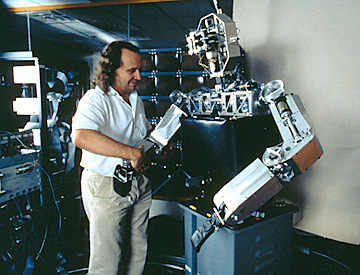
\includegraphics[height=5cm]{brooks_and_cog.jpg}}
    \hfil
    \subfloat[][Cynthia Breazeal with Kismet]{\label{fig:breazeal_kismet}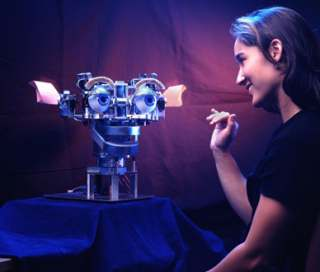
\includegraphics[height=5cm]{breazeal_kismet.jpg}}
    \caption{The Cog project was about the use of computer and robotic technology to better understand and emulate human intelligence.}
    \label{fig:cog_project}
\end{figure}


The context of this PhD thesis is grounded in the same scientific motivations as the work of R. Brooks, R. Pfeifer, T. McGeer and initiative such as the Cog project i.e. \textbf{exploring the role of morphology, cognition and embodiment intelligence in several ways using real experimental robotic platforms}.

The scientific approach of the Cog robots is oriented toward the exploration of embodiment in several ways, from the low level mechatronics to head design for social interactions, but robots were built 15 years ago and using classic manufacturing techniques (see \figurename~\ref{fig:cog_project}) that made them expensive, complicated to modify and especially difficult to diffuse in other laboratories.
We are now in 2014, the makers revolution is in progress~\parencite{anderson2012makers} and novel technologies allow a rethink of the way we design robotic platforms, especially humanoid ones.


In the Inria Flowers team\footnote{\url{flowers.inria.fr}}, we are interested in the study of mechanisms that can allow robots and humans to autonomously and cumulatively acquire repertoires of new skills over extended periods of time. This includes mechanisms for learning by self-exploration, as well as learning through interaction with peers, for the acquisition of both sensorimotor skills (e.g. locomotion, affordance learning and active manipulation) and social skills (e.g. grounded language use and understanding, adaptive interaction protocols, and human-robot collaboration).

With the work An interesting evolution over the last decades has been the demonstration of the importance of robot morphology for sensorimotor control, cognition and development (\parencite{kaplan2008corps} \parencite{steels1995artificial} \parencite{Pfeifer06}). Indeed, robot behaviour cannot be preprogramed. The actual behaviour is always emerging from a complex interaction between the control algorithm, the robot’s morphology and the environment~\parencite{Steels1991emergence}. Moreover, it is clear that a well-adapted robot morphology using specific properties can greatly reduce the complexity of a given task by ensuring implicitly a part -or the entirety- of the control required~\parencite{pfeifer2005morphological}.
Finally, as Rodney Brooks argued, \emph{the world is its own best model}~\parencite{brooks1991intelligence} and simulators cannot realistically handle the complexity of real physics with multi-point contacts, soft material compliance, friction or unpredicted multi-modal interactions.


% \textbf{Needs}

Exploring mechanisms of acquisition requires us to also focus on robot morphology. Therefore, we \textbf{should consider robot morphology\footnote{ robot morphology is defined as any characteristic which defines the physical structure of the robot such as link sizes, number of links, joint characteristics, mass distribution, actuator characteristics, material properties, sensor characteristics and sensor placements~\parencite{paul2006morphological}} as an experimental variable~\parencite{kaplan2008corps} that can be tuned, and conduct experiments in the real world}.

While it is straightforward to explore and experiment with the variation of certain software parameters (e.g. algorithms, simulator), experimenting with morphological variables on a real robot is much more challenging:

\begin{enumerate}
    \item how can we have an experimental robotic platform that allows for morphology to be easily and quickly changed  while acting robustly in the real world?
    \item how can we make this project, mainly the hardware, diffusible and reusable in the research community?
\end{enumerate}

Unfortunately current robotic platforms are not suitable for addressing such challenges.

On one hand, commercial robots such as Nao \parencite{gouaillier2008nao}, Darwin Op \parencite{ha2011development}, Nimbro Op \parencite{schwarznimbro} or iCub \parencite{metta2008icub} are easily accessible and easy to use. Yet they provide a "traditional" morphology (e.g. limited compliance, rigid torso, large feet, over actuation) and modifying their morphology is impractical or impossible. Moreover in most case, they are not open source and/or the hardware is to complicated/expensive to modify.

On the other hand, lab prototypes are mainly handcrafted and specifically tuned which make them almost impossible to reproduce in another lab.

The main issue of these robots is the approaches and technologies chosen to design and produce them. Indeed, the classic way of designing and producing robots is a complicated, time-consuming and expensive process involving specific upfront tooling and complex manufacturing processes.

% \textbf{Task:}

In this thesis, we \textbf{suggest novel approaches and design processes to create and produce robotic platforms,  the control and morphology of which can be freely explored through experimentation in the real world,  that are easy to diffuse and reproduce in the research community.} Especially, this alternative design methodology is driven by the desire to:
\begin{itemize}
    \item freely explore morphological properties,
    \item reduce the amount of time required between an idea and its experimentation on an actual robotic platform in the real world,
    \item makes experiments that should be easy to do, actually easy to do,
    \item make the work easily reproducible in any other lab,
    \item keep the work modular and free to use in accordance with open source principles, so it can be reused and extended for other projects.
\end{itemize}


To reach these goals, we decided to follow novel design methods for both design and production, for all technological aspects of the robot (i.e. mechanics, actuation, electronics, software, distribution). In particular these methods relies on:

\begin{description}
    \item[3D print mechanical parts:] Since few years’ novel techniques, especially 3D printing, are revolutionizing the way we can produce objects. 3D printers open new horizons as they are able to produce parts which were, until now, either not possible or extremely expensive to produce using classical techniques. Especially 3D printing techniques are fast, low-cost and accessible. It allows everyone to produce complex mechanical part in just a couple of hours without requiring any specific upfront tooling.
    These properties of the 3D printing process enable for the first time the exploration of morphological variant for mechanical parts. Indeed, it is now fast and low cost to create alternative design. Associated with modular architecture, we can easily and quickly change robot parts and conduct experiments.
    \item[Electronic architecture based on Arduino] Exploring the role of morphology does not only concern the mechanical properties but also the sensors apparatus i.e. which sensor is used and where it is placed on the body. While it is not yet possible to print complex electronic circuit, we preferred to rely on the Arduino hardware and software environment, which make electronic board easily reconfigurable and compatible with a wide range of sensors. Also, low-level embedded programing skills are not necessary because the board micro-controller can be programmed using Arduino programming language, which abstracts most of the complexity.
    \item[Easy to use python API:] We designed a robust sensory-motor control API adapted to the hardware variability we have. We choose to use Python as it allows fast development, easy deployment on all operating system and quick scripting by non-necessary expert developers. It also offers a large variety of scientific and machine-learning libraries used in robotics (e.g. Numpy, Scipy, Scikit-learn).
    \item[Open source diffusion:] Finally, while the main aspect of such an approach is to allow variability, reuse and modification of the initial design, it is necessary to not only diffuse our work through scientific publications but also to distribute the material needed. This means anyone outside the Flowers lab should have access to the actual source files and be free to make any changes suitable to their own research. Therefore in addition to the technological choices previously presented, we decided to distribute all our work (both software and hardware) under open source licenses. This is an essential step toward building new research tools that facilitate both scientific validation and cumulative science in robotics.

\end{description}

We think this design methodology can contribute to  1) the construction of better experimental robots while making the modification of robot morphology both easy and low cost, and 2) the transfer and reuse of scientific work in other laboratories through the use of open source diffusion.

Within this context we have built a whole new humanoid robot called Poppy\texttrademark (see Fig.~\ref{fig:poppy_with_me}). This humanoid robot was designed to conduct scientific experiments easily and quickly on sensorimotor learning, exploring morphological properties, and human-robot interaction. As an experimental robotic platform, Poppy was designed to be \textbf{affordable}, \textbf{lightweight}, \textbf{robust and safe}, \textbf{easy to use}, \textbf{highly-hackable} and \textbf{fast and easy to duplicate or modify} with the goal of being easily reproducible and used by other labs thanks to an open source distribution (hardware and software).

\begin{figure}[tb]
    \begin{center}
        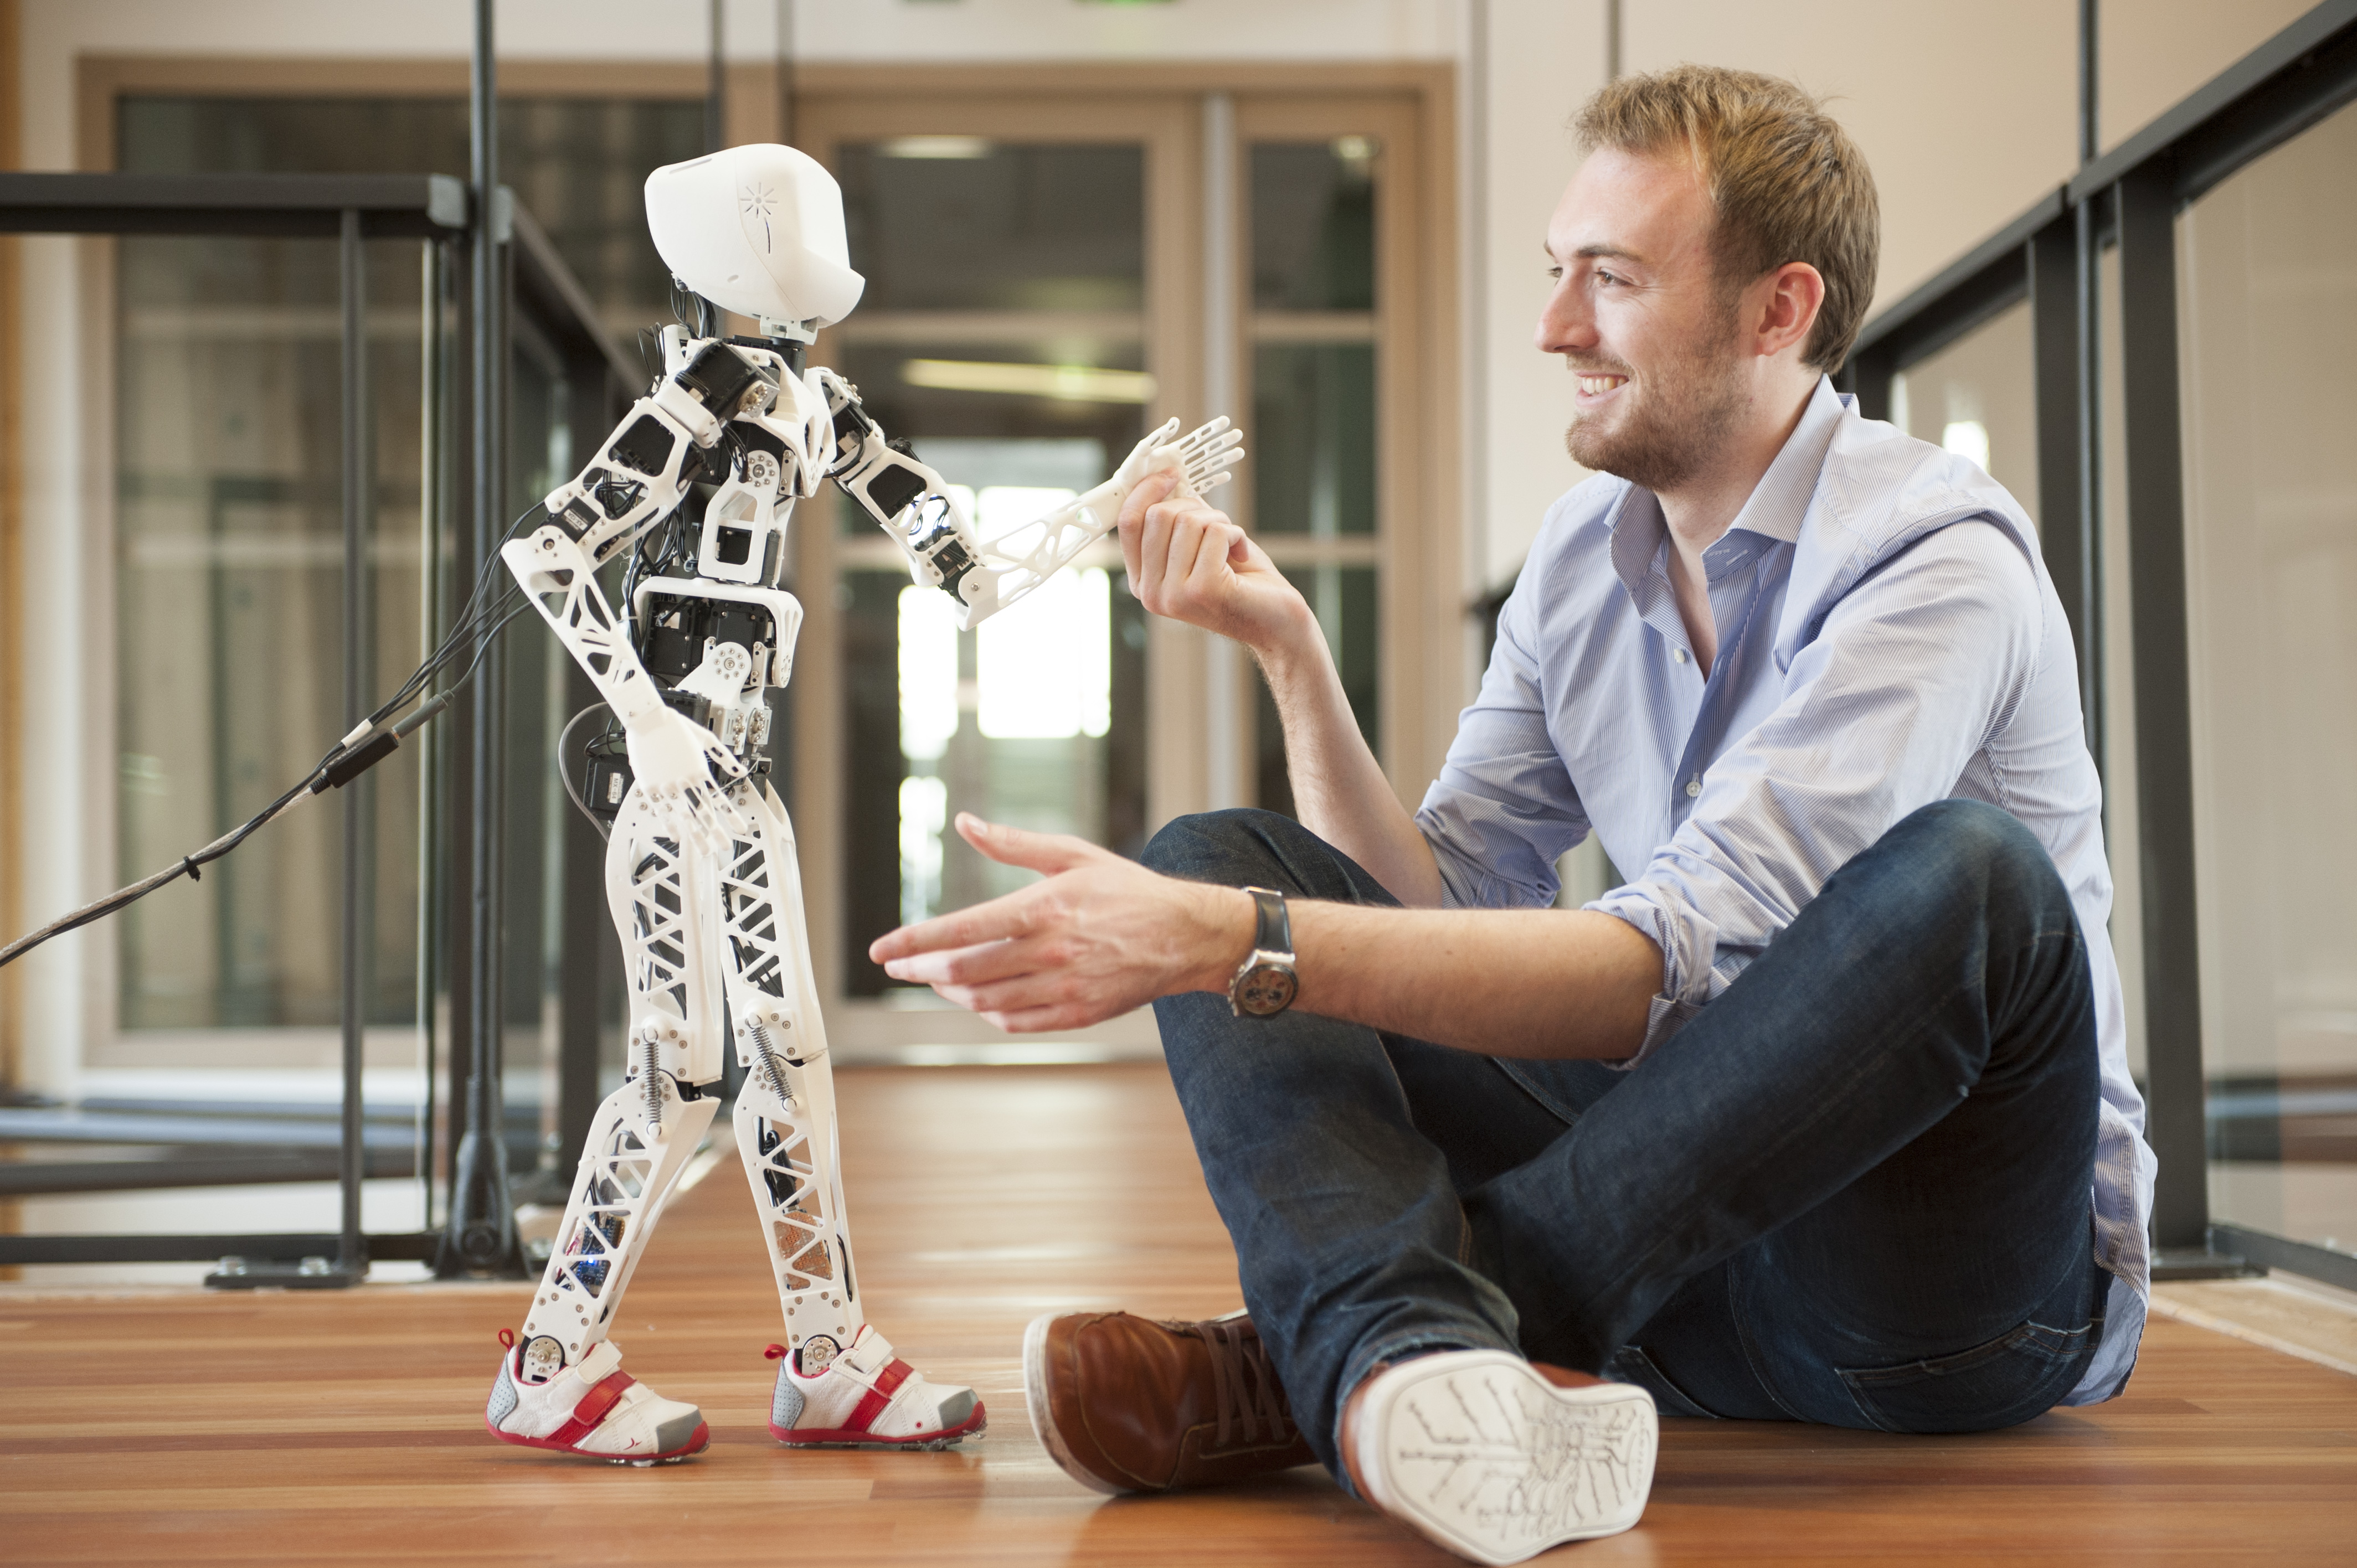
\includegraphics[width=0.7\linewidth]{lapeyre_and_poppy.jpg}
    \end{center}
    \caption{Poppy is a humanoid prototyping platform, which design has been made following the methodology presented in this thesis. It allows for a rich and easy exploration of the robot morphology and its impact on control and cognition. As open source and modular platform, it permits pertinent applications in Science, Art and Education contexts. And is strongly share with open collaboration and cumulative science philosophy}
    \label{fig:poppy_with_me}
\end{figure}

Poppy makes possible exploring new body shapes in just a few days. It enables and simplifies the experimentation, the reproduction and the modification of the morphology in research laboratories. It also allows collaborative working, sharing and replication of the results on these issues between laboratories. The ambition is to become a reference platform for benchmarking and dissemination of scientific results.

Thanks to the fact that it integrates advanced and yet easily accessible techniques in an embodiment that motivates students and the wider public, this platform also meets a growing societal need: education and training in technologies combining computer science, electronics and mechanics, as well as a training tool to the emergent revolutionary 3D printing process. Poppy provides a unique context for experimentation and learning of these technologies in a Do-It-Yourself (DIY) approach. Finally, the possibility to easily modify both the hardware and the software also makes Poppy a useful tool for artistic projects working with interactive computerized installations.


\section*{Proceeding} % (fold)
The proceedings of this thesis will be structured along 4 main parts.

Firstly, a related work will present 1) some inspirational scientific work made over the last 20 years showing the paramount importance of the robot morphology, 2) how we used to design robotic platform until now, and 3) the emergence of the 3D printing techniques and open hardware projects.

We will then describe the development of the Poppy project. In chapter REF we will present the chosen approach to build robotic platform allowing both a free exploration of their morphology and their diffusion in the research community. Then we will present how we used this approach for the design of a novel humanoid platform called Poppy and an easy-to-use robot control library called pypot. We will close this part on the Poppy project's development by the challenges raised by the creation of a research community.

The next part will deal with Poppy's applications and experiments we made about the exploration of morphology (chapter REF) but also for educational (chapter )and artistic (chapter ) purposes.

A discussion part will cloture this thesis. In particular we will discuss potential way to diffuse Poppy and the technological tools we created along this thesis. Following a general discussion of this thesis.


% \cleartoleftpage
% \part{Related Work}
% % !TEX root = ../../thesis.tex

% \cleardoublepage
% \newpage
% \thispagestyle{plain}
% \mbox{}
% \includepdf{/Users/matthieulapeyre/Documents/phd_thesis/media/thebeast.pdf}

Kant les hommes sont comme les oiseaux

\chapter{Robot morphology: some fascinating work} % (fold)

\cleanchapterquote{The cognition needs a body to think}{Rodney Brooks}

\section{The cognitivist approach limits} % (fold)

In 1949, the Elmer and Elsie robots, also known as turtle robots (see \figurename~\ref{fig:walter_robot}), created by the cybernetic pioneer W. Grey Walter, can be considered as one of the first robots in the robotics modern history era (1950-now). Back at this time, the transistor was just invented (1948)~\cite{brinkman1997history} and calculus was done with mechanical machines (see the focusbox). The turtle robot was entirely analogical but was able to demonstrate complex behaviors (see \figurename~\ref{fig:turtle_behavior}). Without any "reflexion" or internal representation of itself and the world, this robot, thanks to its conception and the direct analogical interaction between sensors and actuators was able to avoid obstacles and reach its charing station~\cite{walter1950imitation}. These complex behaviors which can be compared with ones found in nature were in fact done without any kind of intelligence and were actually emergent from interaction between the robot morphology (i.e. where are placed sensors and how they are connected with actuator) and the robot environment (i.e. light sources).

\begin{figure}[]
\centering
    \subfloat[][]{\label{fig:walter_robot}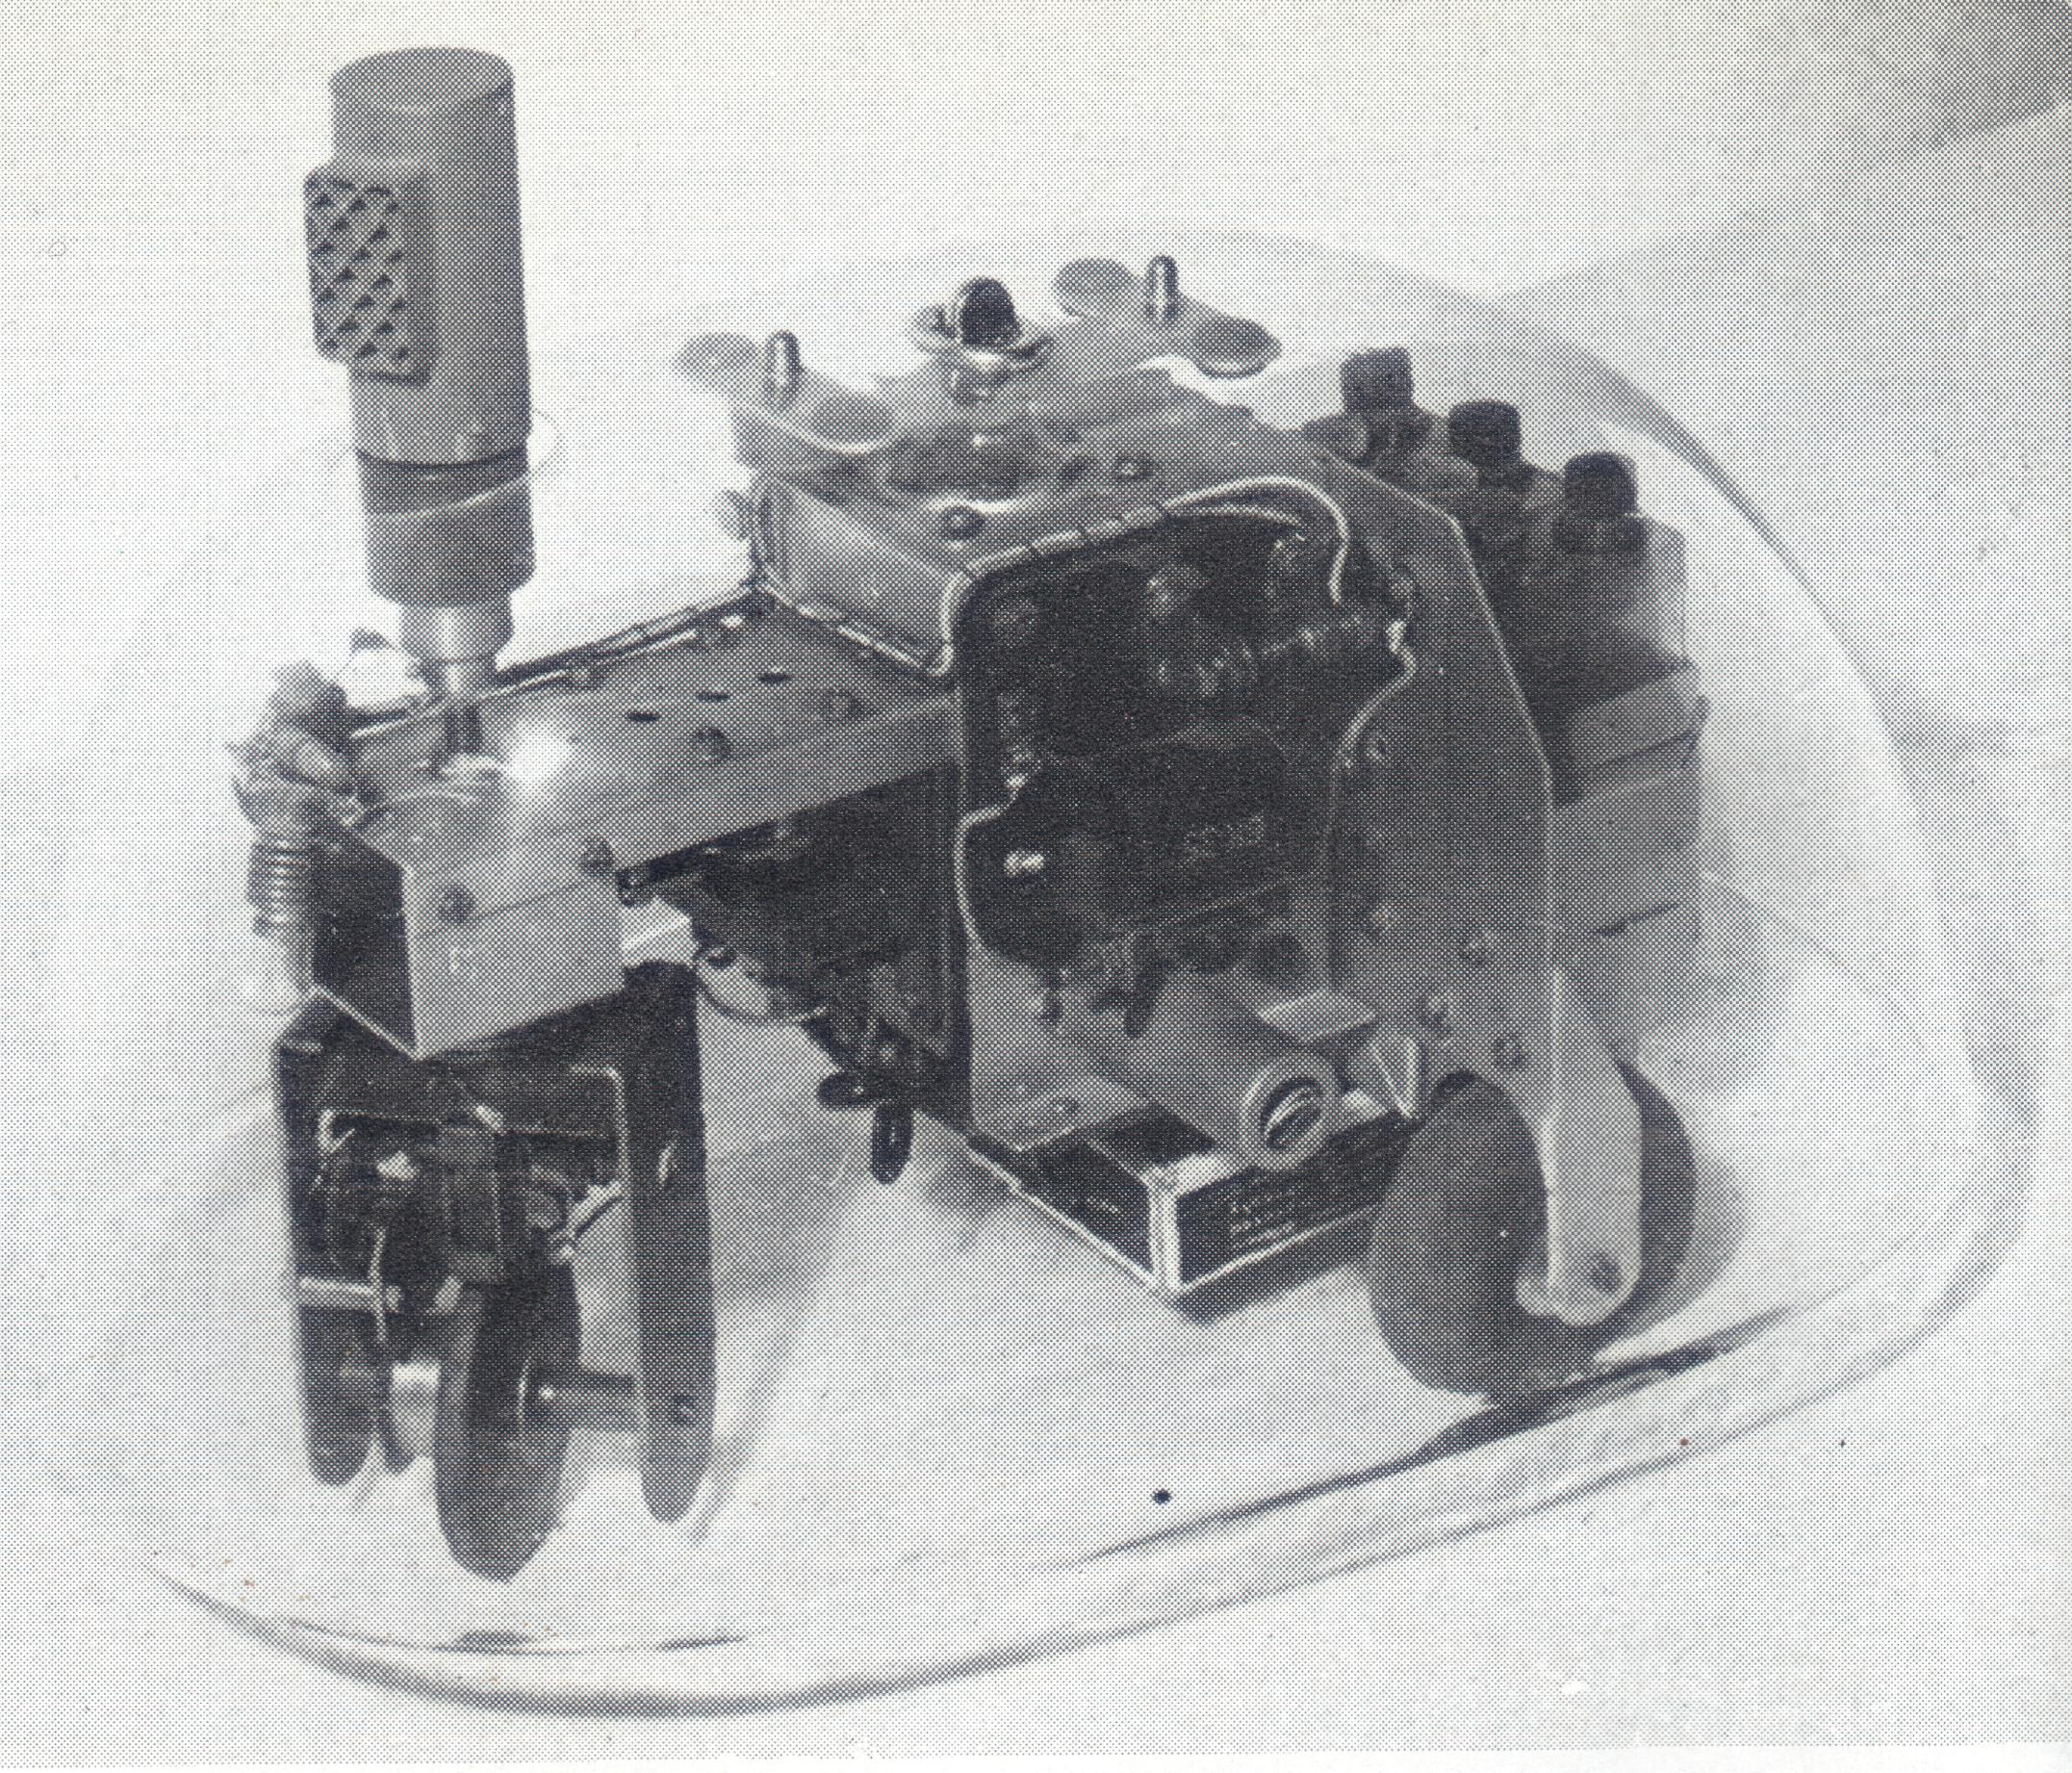
\includegraphics[height=6.5cm]{walter_turtoise_robot.jpg}}
    \hfil
    \subfloat[][]{\label{fig:turtle_behavior}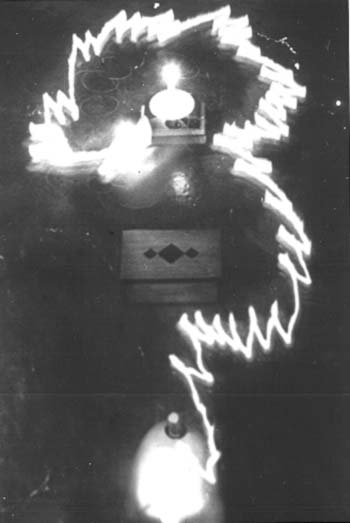
\includegraphics[height=6.5cm]{turtoise_behavior.jpg}}
    \caption{}
    \label{fig:turtle_robot}
\end{figure}

\begin{figure}[]
    \centering
    \begin{boxedminipage}{0.95\textwidth}
        \textbf{Mechanical calculus}\\
        Once upon a time, in a age transistors were not here, complex calculus was done using mechanical properties.
        Using complex mechanisms the very first calculators were fully mechanical machine (see \figurename~\ref{fig:mechanical_computer}).

        The first freely programmable, binary, floating-point, general-purpose mechanical computer in the world was the Z1 constructed by Zuse between 1936 and 1938 (see \figurename~\ref{fig:zuse_z1}).
        This "computer" contained approximately 30,000 components and was incredibly sophisticated, making the Z1 suitable for a wide variety of engineering and scientific applications.
        Introduced by Curt Herzstark in 1948, the Curta (see \figurename~\ref{fig:curta_calculator}) is a small, hand-cranked digital mechanical calculator.
        It can be used to perform addition, subtraction, multiplication, division, and (with more difficulty) square roots and other operations.
        The Curta's design is a descendant of Gottfried Leibniz's Stepped Reckoner and Thomas's Arithmometer, accumulating values on cogs, which are added or complemented by a stepped drum mechanism.
        It has an extremely compact design: a small cylinder that fits in the palm of the hand.

        These two examples show that even pure calculus is achievable using only morphological properties (here mechanical) and was used during dozens of years for scientific applications.


        Curtas were considered the best portable calculators available until they were displaced by electronic calculators in the 1970s.

        \begin{center}

            \subfloat[][Zuse Z1 (1936)]{\label{fig:zuse_z1}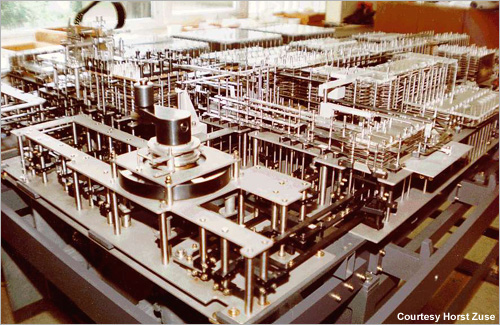
\includegraphics[width=0.42\linewidth]{hist-z1-reconstruct.jpg}}
            \hfil
            \subfloat[][Curta]{\label{fig:curta_calculator}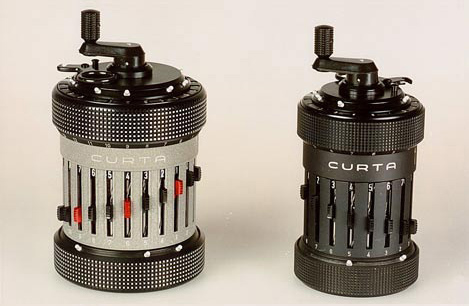
\includegraphics[width=0.42\linewidth]{curta_calculator.jpg}}
            \caption{Mechanical calculus machines}
            \label{fig:mechanical_computer}

        \end{center}

    \end{boxedminipage}
\end{figure}

With the arrival of numeric computers, researchers imagined the opening of a field where it could be possible to replace pre-wired analogical electronic behaviors by the use of computer running programs. Not dependent on the hardware platform, robots would be therefore more versatile.
The artificial intelligence (AI) term was introduced in a workshop organized in 1956 by a MIT professor John McCarthy (REF). Globally participant were convinced, that by using the notion of computation or abstract symbol manipulation, it would be possible to reproduce interesting abilities similar to human ones~\cite{kaufmann1979machines}~\cite{haugeland1989artificial}. The symbol-processing paradigm or cognitivistic paradigm see the cognition as pure computation. In other word, the actual intelligence process is the abstract algorithm or the program doing calculus. Eventually, researchers following this paradigm no longer saw the physical incarnation as a relevant component. Cognitive and computationalists hypotheses stating that the thought is reducible to a set of symbolic calculations are being established~\cite{fodor1987psychosemantics}. The body, for its part, is forgotten, irreparably separated from the mechanisms of intelligence~\cite{kaplan2008corps}.
In addition, the robot body became a handicap which often ruins the efficiency of algorithms and programs created by AI researchers. Indeed, the real world body is non perfect, there is some noise on sensors acquisition, there is gravity, friction and inertia acting on actuators, and the environment is always changing and unpredictable.

To overcome these issues of real world applications, the other side of the robotics community, still interested in the hardware challenges strives to design more reliable and powerful robots which can react as fast and as close as possible to the model used for its control. To do that, it is needed to have way more precise sensors and powerful enough actuators to overcome inertia and mechanical friction. Thanks to these work on hardware, industrial robots became more and more fast and precise, enough to outclass any human on specific assembly tasks.

However, even with really efficient robots, artificial intelligence failed to show results comparable with the expectations researchers and society had. Robots are able to solve incredibly complex task such as chess game or able to achieve highly precise tasks in manufacture but require perfectly controlled and predictable environment. Going outside this known environment seems impossible to program and none of them is able to act fluently in the real world.

Thus classical approach known great successes to solve abstract problems such as chess game, search engine, text processing, however it failed in the understanding of natural forms of intelligence which requires a direct interaction with the real world. This is especially the case when we think in the current state of the art for interaction with human (natural language) or object (grasping) and the locomotion in an open environment (walk, run, ride a bicycle).


\section{The emergence of embodiment paradigm} % (fold)

Stuck with these major issues raised by acting in the real world, a kind of crisis of the artificial intelligence happened in the 1980's and the cognitivist paradigm was questioned. While some researchers of the field introduced new tools such as neuronal networks, another part questioned the "cognition is computation" approach and the irrelevance of the body.
Thanks to researchers such as Rodney Brooks~\cite{brooks1986achieving}, Rolf Pfeifer~\cite{pfeifer2001understanding} or Luc Steels~\cite{steels1995artificial}, a novel paradigm emerge: the cognition needs a body to think. The embodied artificial intelligence rejects the symbolic approach and postulates that it is not possible to have intelligence without the body and the environment~\cite{pfeifer2001understanding}. Rather than postulating there is a hierarchical structure in which the brain control the body, the new theory focuses on the interaction between the two systems, even for mathematical thinking we could assume is purely abstract~\cite{lakoff2000mathematics}.

Following this paradigm, several researchers tried to tackle challenges in which the classical cognitivist approach failed i.e. the understanding of natural forms of intelligence which requires a direct interaction with the real world. The locomotion is a great example of task where the classical robotic approaches did not get expected results.

Animals are incredibly skilled. Even if we consider insect with a brain thousand of times smaller than the human one, theirs abilities to move in an open world is just incomparable with the most advanced current robots. One important reasons for this is that in the classical view, the ability to figure out where you are is based in detailed inner models or representations either have to be programmed into the robots or learn by interacting with the environment and continuously updated. The more complex these models are, the more effort is needed to acquire the relevant data to maintain them leading to major problem when learning task in a highly dimensional spaces (plein de REF). Brooks even argued that intelligence always requires a body and that we should forget about complex internal representations and models of the outside world; that we should not focus on sophisticated reasoning processes but rather capitalizer on the system-environment interaction~\cite{brooks1991intelligence}~\cite{brooks1995intelligence}. Then he started to work on the insect locomotion because if we understand the insect-level-intelligence it will be much easier and faster to understand and build human-level intelligence~\cite{brooks1996prospects}.

\textbf{TODO: petite review du boulot de brooks avec les insects}

Exploring the role of the morphology and how it shapes the ways we think appears a fascinating open field. Indeed, exploring the interaction between body properties and cognition could lead to both a better understanding of animal's behaviors (human being in particular) and to build robot more adapted and robust to an open environment with unpredictable interaction.

Thus an interesting evolution of the last decades is the demonstration of the importance of the morphology for sensorimotor control, cognition and development. The researches community exploring the embodiment paradigm has grown but surprisingly not as much we could imagine with classical paradigm fails. However, new work arises introducing new principles we will describe in this chapter such as morphological computation, compliance or ecological balance, emergence.

In the context of this thesis we will talk about intelligence with the meaning, ability to move in a natural environment and interact with people and objects.


% \begin{figure}[]
%     \centering
%     \begin{boxedminipage}{0.95\textwidth}

%         \textbf{Planes fly only thanks to their morphologies}\\

%         One of the major engineering achievement of the Twenty-th century has been the understanding of the fly and the realization of efficient plane both for commercial and military application.

%         A priori there

%         If we study a complex behavior such as the ability to fly. Using a cognitivist paradigm, the fly would require a large amount of explicit calculus.  With this approach we could think the fly need a large amount of explicit calculus. However the aeronautic people already understand that the plan they are trying to make fly will act in the real world and the real world is the "air". A plane can only fly because of the air and because it is viscous. The air is not a constraints it is the central element for make a plane fly.

%         Indeed a plane has to deal with its environnement which is the "air".

%         % While ones could see the real air as a constraint because of its viscousness and prefer model it as a perfect fluid in simulation, it would be impossible or at least way more complicated to make a plane fly. Indeed, it is because the air is viscous that the fly is possible.

%         Actually a plane fly only thanks to the interaction between its specific wing morphology and the environnment fluid which is the "air".

%         \begin{equation}
%             F_{lift} = \frac12 \times \rho \times V^2\times S \times C_z
%         \end{equation}

%         To create lift, the only variable are the profil shape which give the $C_z$ parameter and the surface voilure $S$ and the air properties with its volumic mass $\rho$ and the velocity of the flux $V$.

%         \begin{equation}
%             adapted morphology + air = fly
%         \end{equation}


%         All the intelliegence is centered around the wing shape.


%         % Another great example of how mechanics properties can produce complex behavior is the airplane.
%         % The lift force generated by wings are the resulting of the interaction between a air flux and the physical profil shape of the wing.
%         % Then the Bernouilli law add the necessary magic around to make plane fly (see \figurename~\ref{fig:magic_plane})

%         we can change the behavior by changing the wing shape, some fighters have a voilure variable

%         Forme des ailes etc ...

%         To resume, a plane can work thanks to the fact the air is not a perfect fluid and because it has an adapted morphology. Even rocket use aerodynamic to improve the stability otherwise it would be really complex to keep a direction.



%         % The only way to make machine "fly" without these specificities is to create a rocket which need a very high power to oppose the gravity and complex control to

%         % \begin{figure}[tb]
%         %     \begin{center}
%         %         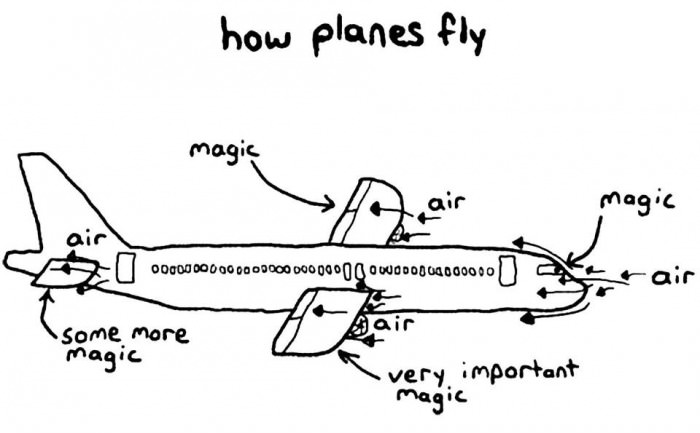
\includegraphics[width=0.8\linewidth]{plane_explanation.jpg}
%         %     \end{center}
%         %     \caption{Caption here}
%         %     \label{fig:magic_plane}
%         % \end{figure}

%         \begin{center}[]
%         \centering
%             \subfloat[][]{\label{}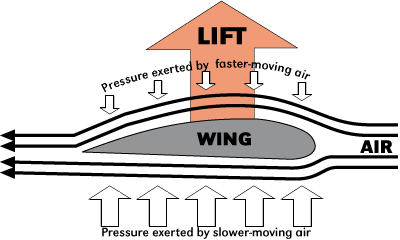
\includegraphics[width=0.4\linewidth]{bernoulli_wing_lift.png}}
%             \hfil
%             \subfloat[][]{\label{}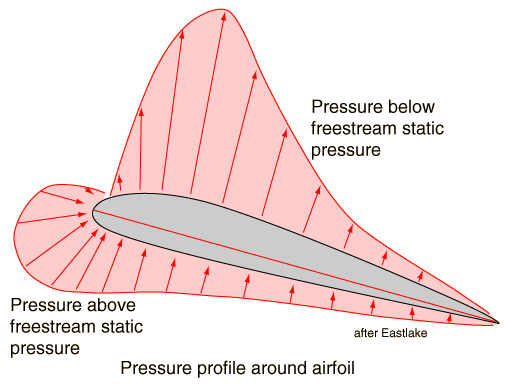
\includegraphics[width=0.3\linewidth]{airfoil_bernouilli.png}}
%             \caption{}
%             \label{fig:}
%         \end{center}

%         After 60 years of fly history with hundreds of actual plane from planneur to airbus A380, it looks obvious that the shape of the plane is a major, or event the most important part. However, then discussing of legged locomotion, from centipedes to biped ones, the question of the morphology is often left aside in favor to computationnal model. Is there really a fundamental reason the body should be irrelevant for legged locomotion while being essential for flying? There is a lot of legged animals and they are not smater than the flying or swimming ones. Is there a fundamental law comparable to the Bernouilli one ? It can be a biological, a mechanical or even a chimical law, yet it deserves to be explored.

%         While the velocity of legged locomotion are in most of the case quite low, we could ignore air friction, then a first track could be the interaction between the newton's law and the ground. Using gravity as an advantage instead of a force we have to battle.

%     \end{boxedminipage}
% \end{figure}


\section{Morphological computation} % (fold)

As we saw in the introduction, with the arrival of numeric computing, the interest for the robot body seemed less and less relevant for artificial intelligence researchers. They used the "think is calculate" paradigm, a cognitivist approach which globally failed in the understanding of natural forms of intelligence which requires a direct interaction with the real world.
However, while we can think there are indeed calculus necessary to achieve complex tasks, there is no reason it should be explicit with a precise internal model or representation of the physical world. Then it could be directly done by through body properties.

Following the definition of the robotic morphology given by C.Paul:
\begin{quotation}
The morphology of a robot thus refers to the physical structure and form of a robot. Specifically, the focus is on characteristics such as link sizes, number of links, joint characteristics, mass distribution, actuator characteristics, material properties, sensor characteristics and sensor placements. In short, any characteristic which defines the physical structure of the robot is included in the term morphology.
\signed{Chandana Paul~\cite{paul2006morphological}}
\end{quotation}

The morphological computation principle states that a part of the computation needed in the achievement of a given task can be done implicitly through the interaction of physical form with the ecological niche environment.

We are particularly interested in this thesis in the role of morphology for the locomotion and interaction in the human ecological niche.

For decades and it is still mostly the case, the challenge of locomotion for robotic agent was only tackles through symbolic abstract and complex computation of internal model and representation of the world. However, regarding the nature, it appears obvious that an animal morphology deeply change the way it can act in its ecological system and so it has evolved trying to optimize its body properties.

For some reasons, in the robotics and artificial intelligence field the link between the body properties and the ability for a robot to move in an ecological environment does not seems as obvious. The fact that the ability to do thing is due to the brain computation is so deeply grounded than it affects even the general public.

Since the 80's, the fact that the morphology of a robot affects its control requirements has become increasingly evident in robotics. Not only does the morphology determine the behaviors that can be performed, but also the amount of control required for these behaviors. Particularly in systems where behavior is obtained through purely sensory-motor interactions of the body with the environment, the morphology is of prime importance. Nonetheless, even in other robotic systems, a relationship has been found to exist between morphology and control requirements, in that some morphologies yield themselves to being more easily controlled than others.

This relationship was first observed and characterized by Pfeifer as the morphology and control trade-off ~\cite{pfeifer2001understanding}, but the mechanisms underlying this relationship have been unclear. The fact that simple physical interactions give rise to computation indicates the theoretical possibility for the dynamics of the morphology to play a computational role in the system, and thereby to subsume part of the role of control~\cite{paulinvestigation}

However, beyond the animal kingdom evidence, the human being already understood this principle in other domains. As in this thesis we are more concerned about the locomotion, we can cite all the vehicules allowing human to locomote in various way invented. Most of the vehicule we used today were invented before the apparition of computer science and were totaly functionnal without any kind of explicit computationnal intelligence.

A car, for example, is an autonomous system able to move in wide range of environnement from perfect asphalt circuit to deep jungle mainly thanks to the damper it has. There is no computaiton of the correct wheel position given a model of the external world and a planning path. The position is just due to the interaction of the car damper properties and the ground.

Another great example is the plane. Make a machine fly is one of the great scientific and engeenering example acheived thanks to a deep understanding of the interaction between the environnement and the morphology.



\subsection{Passive and Semi-Passive Walkers} % (fold)

Tad McGeer


This set-up the work of Tad McGeer, comming from the aeronautic field, he was surprised by how the actual legged robot morphology was neglected. A great example is the Tad McGeer's passive walker. Thanks to the understanding of the intrinsic dynamics of its structure, Tad McGeer has managed to create a 2D biped robot capable of producing several steps without any controller or motor showing that such a complex task can be indeed achieved only with adapted morphology\cite{mcgeer1990passive}.

The result is comparable to the sailplane or the paper plane. Using a specific mass repartition and foot shape interecting with gravity and the ground ...

The role of morphology in robot biped locomotion has been particularly explored through the research on passive dynamic walkers~\cite{wisse2007passive}.
The most famous example concerns the Tad MacGeer's work~\cite{mcgeer1990passive}.
Thanks to the understanding of the intrinsic dynamics of its structure, McGeer has managed to create a 2D biped robot capable of producing several steps without any controller or motor.
The only control of this robot is obtained through the interaction between the intrinsic inertia of the structure and gravity.

\begin{figure}[]
\centering
    \subfloat[][Tad McGeer with his prototypes]{\label{fig:tad_mcgeer}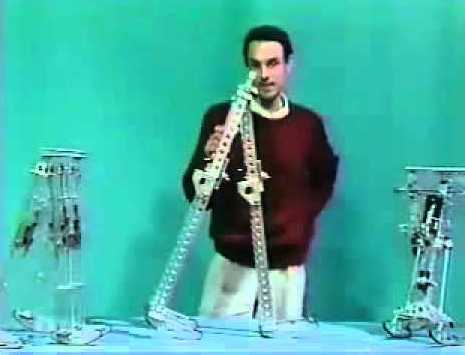
\includegraphics[width=0.49\linewidth]{tad_mcgeer.jpg}}
    \hfil
    \subfloat[][Passive walker robot]{\label{fig:mcgeer_walker}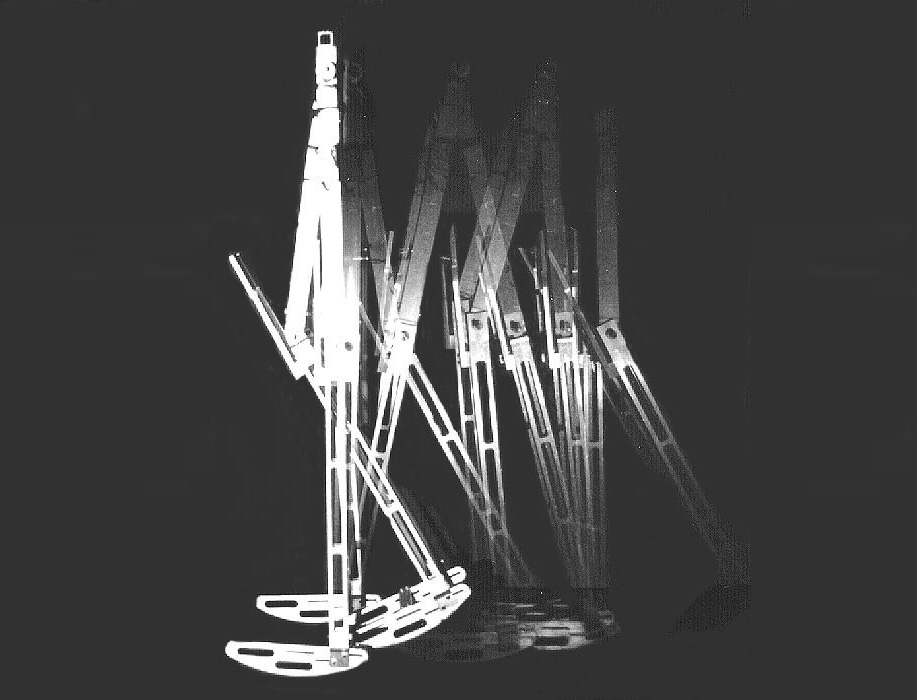
\includegraphics[width=0.49\linewidth]{mcgeer_walker.jpg}}
    \caption{}
    \label{fig:mcgeer_work}
\end{figure}

This work has been pursued with the apparition of semi-passive walker combining both specific passive properties and low power actuation to increase their robustness~\cite{Anderson2005}.
We can note the work of Collins~\cite{collins2005bipedal} which explored the case of semi-passive 3D biped robot.
Its morphology is based on particular mass distribution, knee locking, round feet and springs on the legs to generate an efficient walking gait while keeping its lateral and frontal balance.
The concept of 3D semi-passive robot has been pushed even further with the realization of a complete humanoid robot with trunk, arms and head: the robot Denise~\cite{wisse2005three} and Flame presented in~\cite{Hobbelen2008}.

http://tensegritywiki.blogspot.fr/2010/08/mechanism-as-mind-tensegrity-and.html

we could make a parrallel the energy consumed to th
\begin{figure}[]
    \begin{center}
        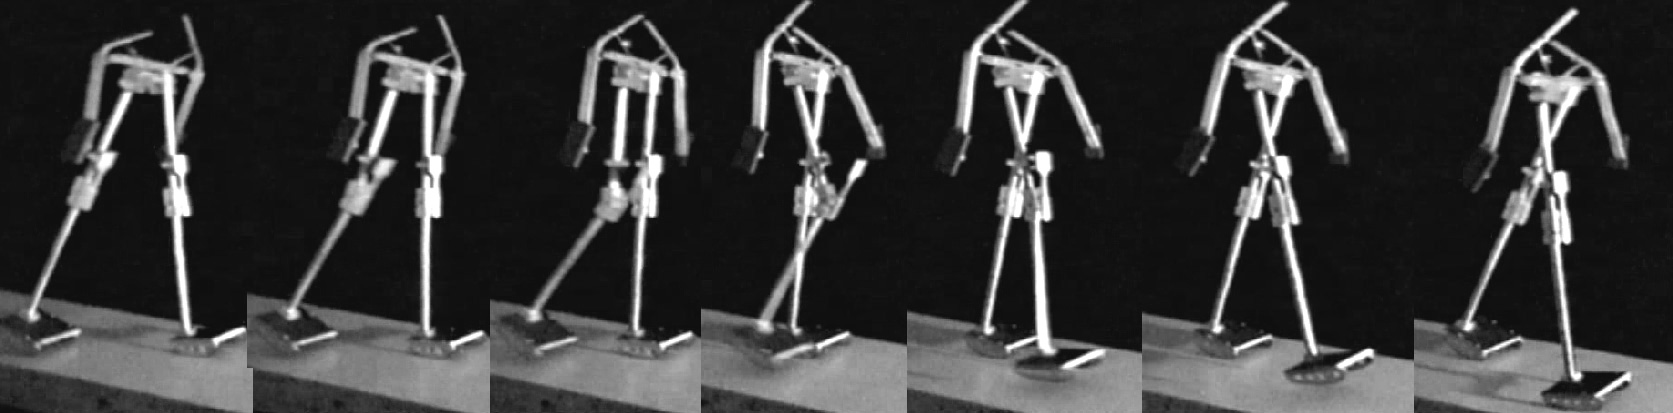
\includegraphics[width=0.99\linewidth]{cornell_biped_series.jpg}
    \end{center}
    \caption{Caption here}
    \label{fig:figure1}
\end{figure}

\begin{figure}[]
    \begin{center}
        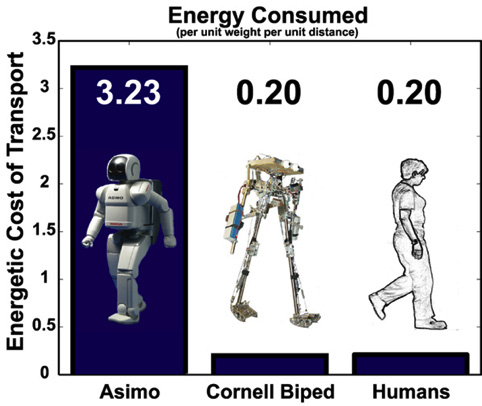
\includegraphics[width=0.6\linewidth]{comparison_cost_transport.jpg}
    \end{center}
    \caption{Caption here}
    \label{fig:figure1}
\end{figure}

\subsection{humans} % (fold)
\label{sub:humans}

% subsection humans (end)
It has also been shown that human morphological properties such as the compliance of the body explains the dynamics of walking and running \cite{Geyer2006} while experiments made by Kojiro Matsushita~\cite{matsushita2005locomoting} show that an adequate morphology is needed if one is interested in natural looking kind of locomotion.


\section{The compliant and soft robotics} % (fold)
It has also been shown that the compliance of the body explains the dynamics of walking and running \cite{Geyer2006} and several biped robots such as Athlete Robot \cite{niiyama2010athlete} or BioBiped1 \cite{radkhah2011concept} were designed using compliant actuator or elastic material.

\section{Ecological balance}

The concept of morphological computation has also been associated to the principle of “ecological balance”, as outlined by Pfeifer et al.\cite{pfeifer2005new}, which states that there is a balance or task distribution between morphology, materials, control, and interaction with the environment.

\section{Emergence of complex behavior} % (fold)

\subsection{The sandbeast} % (fold)

We should not only interest ourself
Some very interesting proofs of concept can be found in the complen

In Art, complementary work can be found. It is the case of The Jansen genius artist. Outside the research community, we can find


\begin{figure}[]
    \begin{center}
        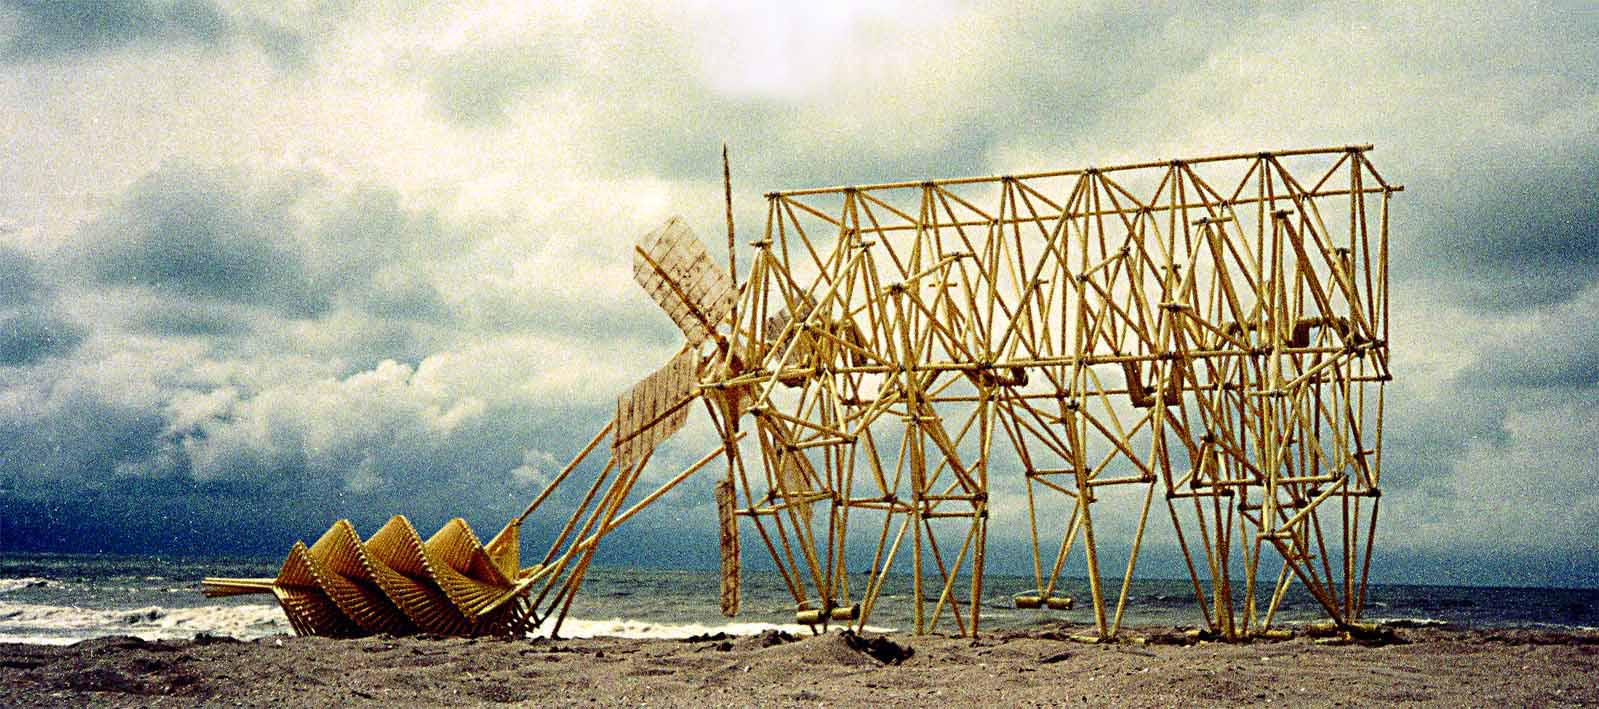
\includegraphics[width=0.99\linewidth]{theo_jansen_beast.jpg}
    \end{center}
    \caption{Caption here}
    \label{fig:theo_jansen_beast}
\end{figure}

Theo Jansen is a sculptor in the kinematic art field. This artist playing with field frontiers, between engineering, research and art is the designer of the sand beasts (see \figurename~\ref{fig:theo_jansen_beast}).
These giant structure move using a really clever mechanisms composed of eleven rods which lenghts have benn tuned through optimization. This system produces a walking motion(see \figurename~\ref{fig:beast_mechanism}) with the center always remaining at the same level, for this reason Theo Jansen likes to say he "reinvented the wheel" but adapted to the environmental niche of his creatures, the beach.

During the XX years of this work, Theo Jansen created dozens of creatures, more and more evolved. However, the very basic mechanism remains the same, both simple because it is composed by only one degree of freedom, and complex because the length ratio between links are critical and must be equal to specific numbers The Janson called gold or god numbers.

Thus, using only really basic material, electric plastic tubes, Theo Jansen created multi-legged creatures capable of moving in the sand, powered by the wind.


\begin{figure}[]
\centering
    \subfloat[][]{\label{}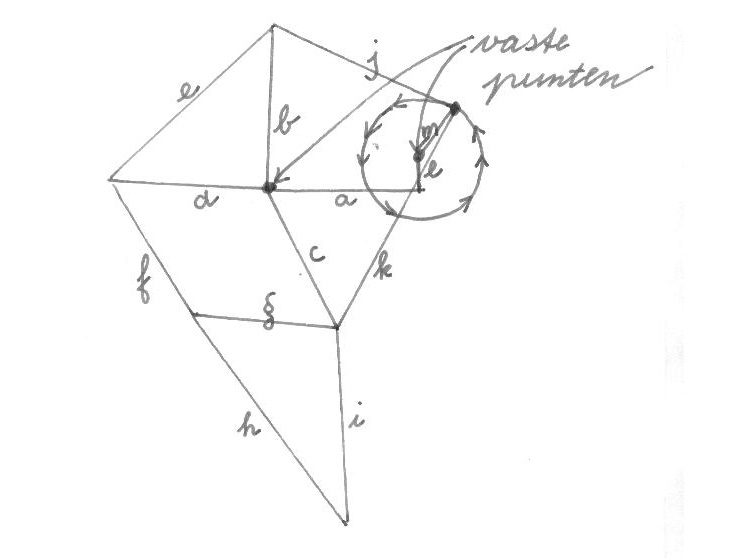
\includegraphics[width=0.32\linewidth]{strandbeest_theory.jpg}}
    \hfil
    \subfloat[][]{\label{}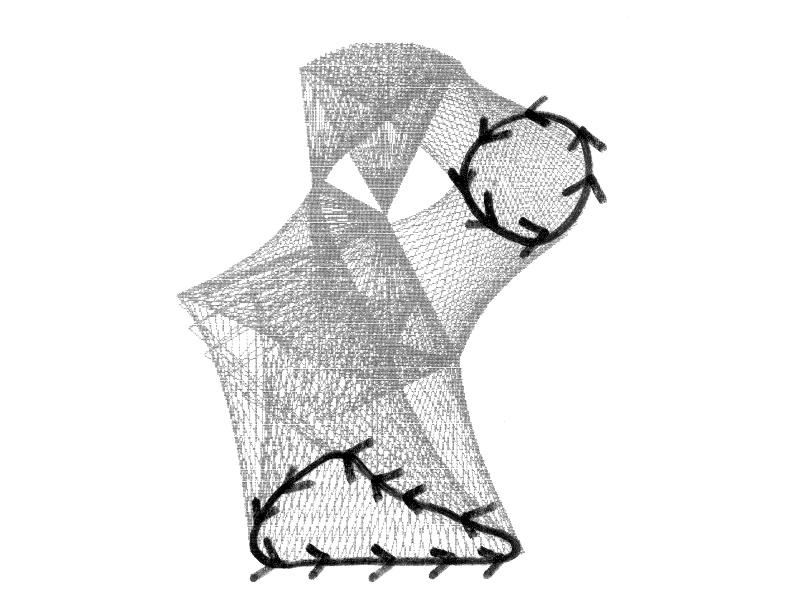
\includegraphics[width=0.32\linewidth]{strandbeest_motion.jpg}}
    \hfil
    \subfloat[][]{\label{}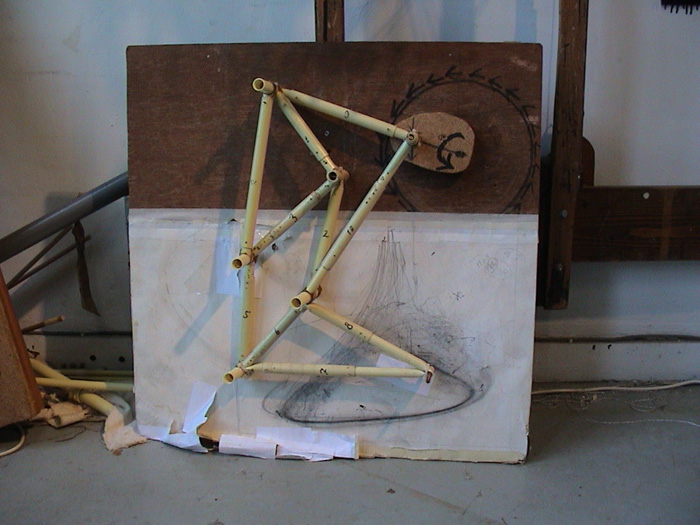
\includegraphics[width=0.32\linewidth]{strandbeest_leg_element.jpg}}
    \caption{}
    \label{fig:beast_mechanism}
\end{figure}



Evolution of his work, conducted to several improvements. For instance, he added lemonade bottle to store energy. These bottle are used as pressure tank fulled using pumps powered by the wind. Beasts can use this stored energy in case the wind fade away.

Also, a natural enemy of these beasts is the sea, using the same basic material, Theo Jansen created sensors able to detect the water and reverse the way beast move. The same principle allows also these beast to avoid obstacle.

Thus the work of Theo Jansen goes beyond the kinematic art and is really instructive for the robotic and IA research fields. Indeed, thanks to a specific morphology adapted to their environmental niche, his creatures are able to act autonomously and "survive" in the real world. No computation, no abstraction, the appeared intelligence of these creatures only came from a direct interaction between their particular morphologies and the environment. It is, for me, a meaningful proof of concept.

\url{https://www.youtube.com/watch?v=rWbU3eV4ZpQ}
72 legs moving at the same time using one cranks

\subsection{Acroban} % (fold)
\label{sub:acroban}
Among all robots designed to explore morphological computation and compliant body only few allow to explore physical interaction such as Kenshiro \cite{Asano2012} or Acroban which the compliant structure of its vertebral column and legs was shown to permit a self-organized physical human-robot interface allowing non-expert users to lead the robot by the hand \cite{Ly2011bio}\cite{Oudeyer2011}.
% subsection acroban (end)

\subsection{Ijspert} % (fold)
\label{sub:ijspert}

% subsection ijspert (end)
PARLER DE LA SALAMANDRE DE IJSPERT
For example, morphological computation has been shown to be necessary in order to achieve human-like biped locomotion \cite{matsushita2005locomoting} and the coupling of adequate morphologies with central-pattern generators has been shown to generate robust locomotor behavior \cite{ijspeert2007swimming}\cite{steingrube2010self}.








\section{Robotic} % (fold)
For years, artificial intelligence was only considered through complex computation.
An interesting evolution during the last decade was the emergence of work showing the importance of the actual robot morphology in the robot behavior.






These robots showed interesting hopping and running behavior while using less power actuator than common humanoid robot such as Asimo or HRP-2.



The morphological properties of these robotic platforms are especially interesting but unfortunately they are difficult and expensive to reproduce by other research laboratories.
Most of the studies made on the humanoid robot locomotion in the past 30 years~\cite{park1998biped}~\cite{aoi2005locomotion}~\cite{park1998biped} mainly focus on tackling the challenge of biped walking through the active control of the whole robot dynamics using technics such as ZMP control~\cite{vukobratovic2004zero} requiring very precise and high torque actuation~\cite{akachi2005development}.

The properties of the robot morphology have shown interesting results for robust locomotion, for instance the hexapod robot Rhex~\cite{saranli2001rhex}.
Still, it is surprising that only few explored the challenge of biped locomotion through the study of the role of morphology.
One can cite the work of Chandana Paul and Josh C.Bongard~\cite{paul2001road} and Ken Endo~\cite{endo2002co} which have explored evolutionary optimization on robot morphology to achieve stable biped locomotion.
They have showed a strong impact of the morphology on the walking behavior and were able to reduce the complexity of the controller by finding good mechanical properties (limbs length and mass distribution).


\section{Conclusion} % (fold)

Scientific study of the role of morphology in sensorimotor control and cognition: in Robotics (McGeer, Pfeifer and co.), in relation with Cognitive Science (e.g.
http://www.pyoudeyer.com/IEEETAMDOudeyer10.pdf ) and animals (e.g.
work of Robert Full)

EmbedIT – An Open Robotic Kit for Education
\url{http://www.eucognition.org/index.php?page=tutorials}




\section*{stuff}
Cognition from the bottom up: on biological inspiration, body morphology, and soft materials Rolf Pfeifer1, Fumiya Iida2, and Max Lungarella3

http://spectrum.ieee.org/automaton/robotics/robotics-hardware/fast-running-biped-robot-based-on-velociraptor

http://spectrum.ieee.org/automaton/robotics/robotics-hardware/japanese-quadruped-robot-pneupard

\section*{stuff to put inside from Pfeifer book}

p44. In the mid-90s, Brooks argued that we have now achieved the "insect level intelligence". Ghengis, Attila et Hannibal, three of Brooks six-legged robots have achieved impressive walking performance in terms of obstacle avoidance and walking over uneven ground. However, insects can do many more things such as navigation or manipulation.

Speak about the Cog project: development of humanoid robot with the goal of eventually reaching high-level cognition.

p45. The term humanoid robot is used for robots that typically have two arms and legs, a torso and a movable head with vision system and sometimes additional sensory modalities such as audio and touch. They are called humanoid because ther is a superficial visual resemblance to humans.

p45.Because of their anthropomorphic shape, people have a strong tendency to project humanlike properties onto these robots. David McFarland's reference to anthropomorphization as an incurable disease.


p55. The synthetic methodology states that by actually building physical agents -real robots- we can learn a lot about nature of intelligence. Physical agents by bringing together results from all the different areas have a highly integrative function. In addition, they allow for concrete testing of ideas in an objectif way: a robot either works or it does not.

p78.The synthetic methodology "understanding by building". We build a system that mimics certain aspects of the behavior we wish to study. This way of proceeding has proved enormously powerful: because you have to build somethong that actually works in the real world, there is no way of glossing over details, which is possible when you formulate a theory abstractly.
Grey Walter's turtles and Braintenberg's vehicules illustrate a very important and a t first quite surprising result: very simple brains, in the right context, can produce seemingly complex behavior that we might even want to call intelligent.


The boids flock on the basis of three simple local rules of interaction: collision avoidance, velocity matching or alignment, and flock centering. p220
The results of experience is amazing given the simplicity of the rules.

Given a certain desired behavior, devising the rules that will lead to the desired behavior is more difficult than explaining the behavior if the system is run i.e if the agent interacts with its environment. THis is called design of emergence (Steels 1991) and it is still an open questoin how this can be done systematically. At the moment, design for emergence is an art rather than a hard-core enginnering discipline. Because the fact that the behavior itself cannot be preprogramed but is always the result of an agent-environment interaction, we must design for emergence rather than directly for a specific behaior.
Evolutionary roboticist Inman harvey of the University of Sussex is right when he proclaims "design is out, evolution is in!". suite p87

Unlike virtual workds, the real-world challenges an agent in various ways. First, because real-world agents are emboied, acquisition of information always take time. Second information thatn an agent can acquire about real world is always very limited. We can never have complete information. This situation is different from a formal game like chess, where knowledge of the board positon constitutes all the information about the state of the game. Third information acquired trhough them will always contain errors. Fourth the real world s not characterized by clearly defined, discrete  states, the weather is never simply goof or bad.
The real wolrd has its own dynamics -things out in the world happen even if not do anything- ther is always time presure due to ongoing change. Thus agent are always forced to act whether they want to or not.
Related to this point, the real world is a highly complex dynamical system, making it intrinsically unpredictable because of its nonlinear nature and its sensivity to initial conditions (hebert Simon has coined the term bounded rationality to designate, in essence, decisions that have to be taken under such circumstances (Simon, 1976,1969e)).


% % % !TEX root = ../../thesis.tex

% Photo Yves Gellie
\cleartoleftpage
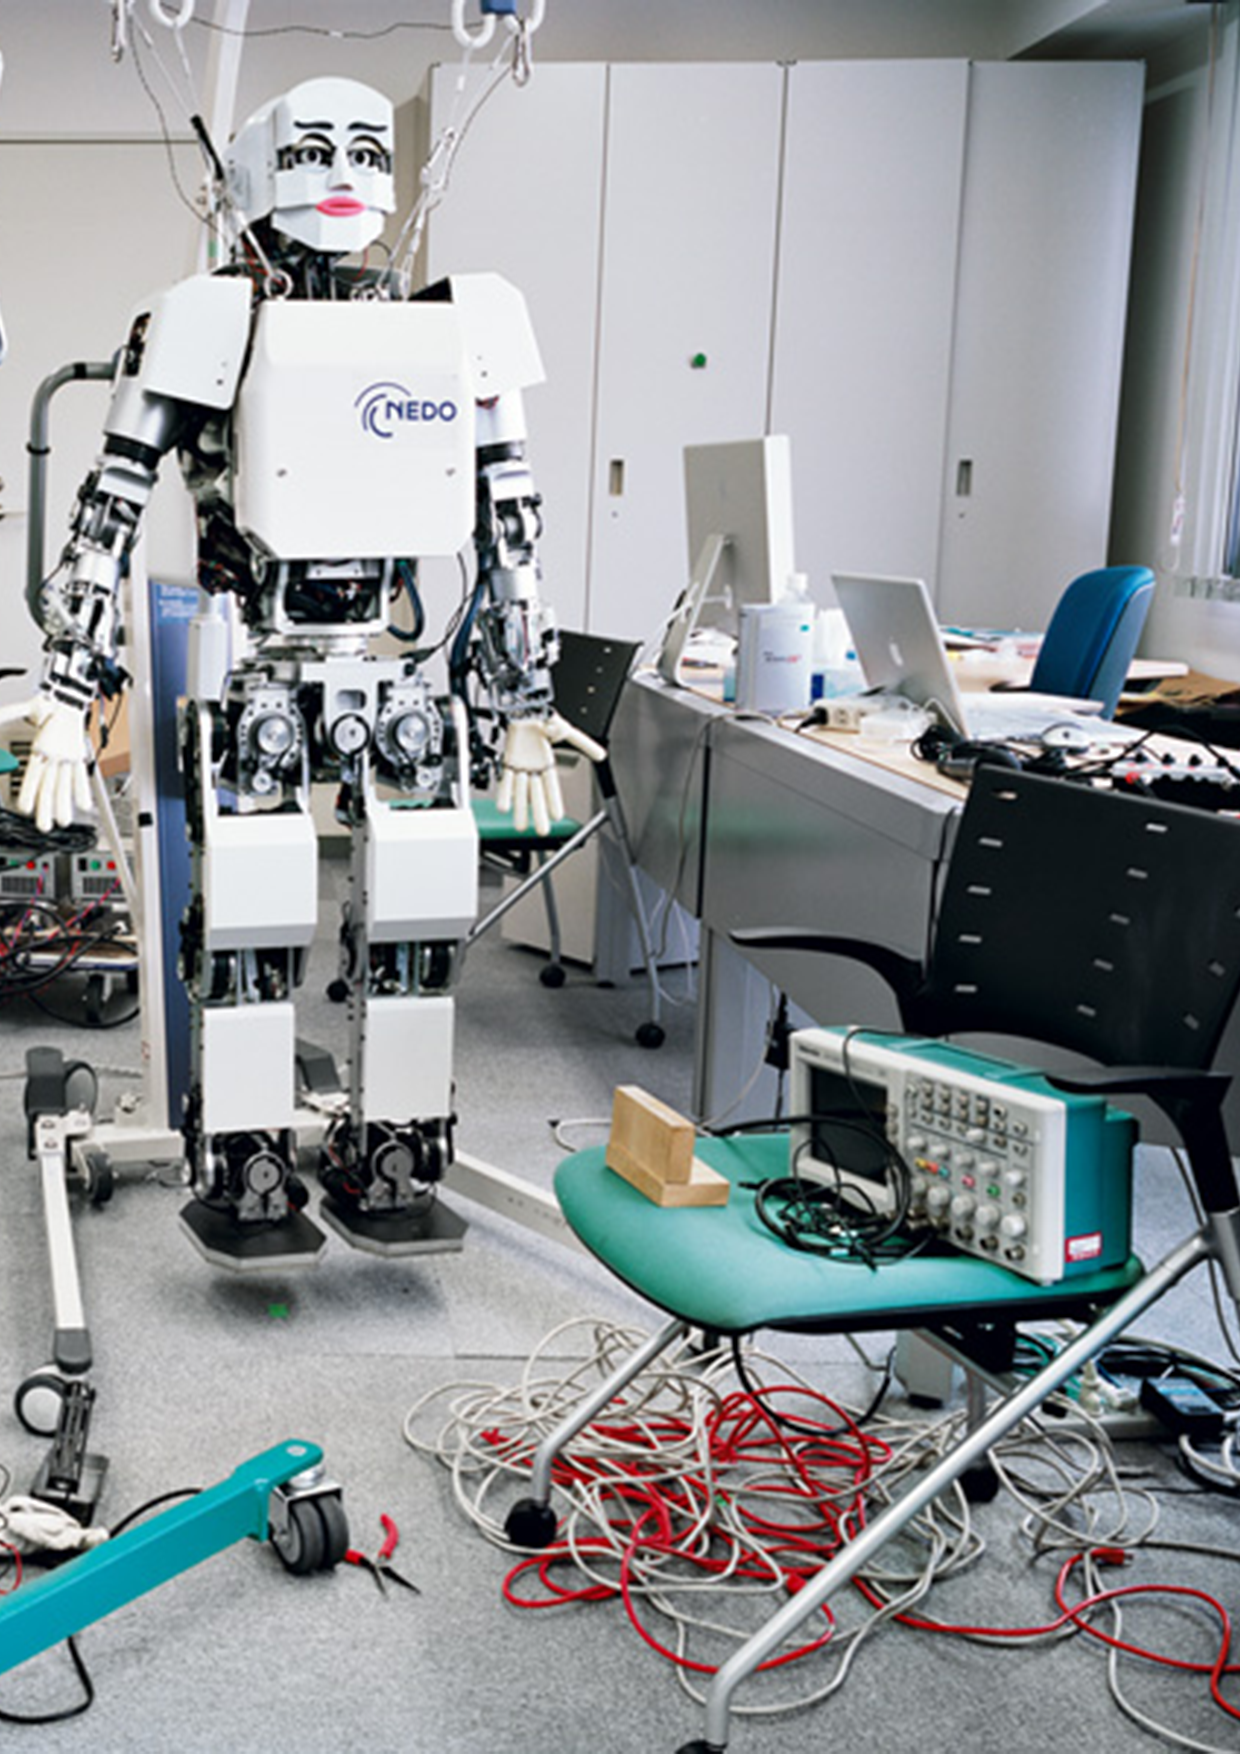
\includepdf{../media/chapter_illustration/robot_setup.pdf}
\chapter{Review of experimental methods} % (fold)
\label{cha:experimental-methods}
\cleanchapterquote{The world is its own best model}{Rodney Brooks}


\section{Introduction} % (fold)

As we saw it in the previous chapter REF, an interesting evolution of the last decades is the demonstration of the importance of the morphology for sensorimotor control, cognition and development. The role of the morphology appears as a fascinating open field. Exploring the interaction between body properties and cognition could lead to both a better understanding of animals’ behaviour (human being in particular) and to build robot more adapted and robust to an open environment with unpredictable interaction.

However as Rodney Brooks explained, exploring interaction between morphology, cognition and environnement requires real world experimentations. Indeed embodiement artificial intelligence REF needs to act in the real world to permit the emergence of complex behavior. The real world includes a large amount of constraints such as inertia, multi-point physical contacts, unpredictable environnement or friction which are, at this time, too complicated to be modeled in physical simulator. Actually "The world is its own best model" and if we can use simulation for exploring basic concepts, the exploration of emergent complex behavior based on interaction between robot self-dynamics and the environnement can only be done through experimentation with real robot in real world.


A great example of achieving complex behavior using robot dynamics is the passive walking (see REF). One of the best sate of the art in this domain is the work done by Delft with the different passive and semi passive walkers they built.

Desiring to explore biped locomotion with Poppy, I had a discussion with Martijn Wisse on simulation strategy to add semi-passive abilities to Poppy. Here is his answer:

\begin{quotation}
First of all, we never actually produced a high-fidelity simulation. We made very simple simulations only. From them, we learned how to tune parameters. Then, we designed the real robots, without running full-blown optimizations. Rather, we used our intuition for a large number of decisions on design trade-offs, using lessons from the simple simulations combined with other limitations such as available motors etcetera. Then, we (again) used our intuition and large amount of experience to tune the robot’s controllers, and make design improvements, until it walked.

\signed{Martijn Wisse - Associate professor at Delft University of Technology}
\end{quotation}

But maybe the most interesting part concerns the work they did to try to make their robot walk in simulation:

\begin{quotation}

Even after obtaining a successful walking motion, we did not manage to create a simulation that walked successfully using the same controller parameters. We tried very hard with some of the best people, but we didn’t succeed. The reason was, I think, that our type of control (using the emergent behavior of a set of simple reflex-like controllers) was highly sensitive to hardware effects like friction. Normally, one uses a local joint controller to make the joint follow a desired trajectory independent of the exact amount of friction. The local controller “abstracts these hardware effects away”, if you know what I mean. This makes the behavior of the whole system quite predictable. However, in our robots, we did not have this kind of abstraction as we were not following trajectories, and thus a little bit of extra friction has an effect on the entire motion.

We did spend a long time making a high-fidelity model in Adams, and also using other methods, but eventually we gave up without success.

\signed{Martijn Wisse - Associate professor at Delft University of Technology}
\end{quotation}


In this chapter, we will review the current state of the art in experimental robotic platforms (see REF). Then we will see how current researcher create robot to explore morphological properties.

\section{Experimental platform} % (fold)

To explore cognition robot need a physical body and to interact with the real world.


There is plenty of robotics platform, from robot arm (Jako, LWR, Kuka) to wheeled platform(Pioneer 3-AT, P3-DX) or even submarine(AQUA2). However, we in this Phd thesis we are particulary interested by the locomotion so we will restraint the review to bipedal platform.

\subsection{Ready-to-use humanoid robot solutions} % (fold)


DarwinOP c'est comme Poppy mais pas forcement pensé pour explorer le role du corps.

\subsubsection{Prototype} % (fold)

\subsection{Commercial} % (fold)

Aside the robot prototype,

Darwin \cite{ha2011development}

Other current research platforms are easily accessible and easy to use such as Nao \cite{gouaillier2008nao}, Darwin Op \cite{ha2011development}, Nimbro Op \cite{schwarznimbro} or iCub \cite{metta2008icub}.
Yet, they provide a "traditional" morphology (e.g.
limited compliance, rigid torso, big feet, over actuated) which can not be easily modified.
It makes them unadapted to study the impact of the morphology on biped locomotion and human physical interaction.

Each of these platforms provides key features for robotics but none of them regroups all the ones needed to explore both biped locomotion and physical interaction.

\section{methods for building robots} % (fold)
icub~\cite{tsagarakis2007icub}

\subsection{Actuation} % (fold)


\subsubsection{wire-driven} % (fold)

\subsubsection{Serie Elastic Actuator} % (fold)

\subsubsection{Pneumatic artificial muscle} % (fold)

\subsubsection{Hydraulic linear actuator} % (fold)


\section{Small humanoid robot} % (fold)
Research on humanoid robot is triving and had lead to a lot of humanoid robot.

We can cite Asimo has one of the first most advanced humanoid robot.

Despite this large number of humanoid platform only few reached a commercial distribution.
Among them there is only one adult sized robot, HRP2 while other are kid-size humanoid robot.

Darwin-OP was one of the first affordable and open source humanoid robot.
Based on the need in lab to have small  humanoid robot for research application.

For some reason, A 3D clone http://www.thingiverse.com/thing:9793
http://www.instructables.com/id/Robot-Cloning-by-DIY-3d-printers/
http://www.instructables.com/id/3D-Printed-Humanoid-Robot-for-under-100000-USD/

Darwin OP has not been really hacked.
Maybe it is due to the tools used.
SVN sucks, sourceforge is outdated.
The open community is more github centered


\section{Current limitations}

In the previous chapter, we presented several works showing the importance of the robot morphology and the need to continu the research in this domain.
However, we saw that none of the available commercial robot platform permits such scientific exploration.

Also, the current research practices in the Robotics field limit the diffusion and the impact of contributions.
Indeed, in most cases, there is no material associated with a published paper.
Meaning, only the theory is shared with the community but not the actual framework allowing to reproduce the results.

\begin{itemize}
    \item Lost of time, design a whole new robot.
    \item Morphology as an experimental variable
    \item Current robotic platforms do not permit to explore the morphology as a variable.
    \item IA haut niveau qui peut se faire en simulation avec certaines reserves.
    \item Currently, robot platform are not satisfying if we want to explore the role of morphology.
    They are not hackable and proto or not both easy to use and accessible.
    \item Problem with simulator VS real world
    \item Exploring control with real robot raise challenge due to error
    \item Morphologie as variable experimental
    \item Engineering on the platform not research
    \item There is two categories, commercial platform and research lab prototype.
    \item No distribution of the code
    \item no benchmark platform
    \item no hackable platform
\end{itemize}

This raises limitations for:
\begin{itemize}
    \item verifying the quality of the results presented in the paper,
    \item the reuse of the contribution as there is, in most case, a gap between the theory and the actual implementation,
    \item the collaborative work with other laboratory
\end{itemize}

However in the context of exploring control algorithm or studying the role of morphology, the actual robot is needed.
Also in this context, it raises major issue concerning the way to share material associated to a scientific contribution.

In this chapter, we present a design methodology allowing to:
\begin{itemize}
    \item consider the morphology as an experimental variable.
    \item easily share our results with the scientific community
\end{itemize}


Similarly to the Locomorph project~\cite{locomorph} which offer a multi-purpose hardware kit allowing to quickly create robot and study the impact of several morphological properties such as link length, joint stiffness or mass distribution, we explored how we could build novel kind of robotic platform allowing to quickly tune morphological parameters.

\section{methods for dissemination and reproducibility} % (fold)

The most common way to  research

Share science

Currently most of the research dessiminatino is done through paper publications.
While papers are a high quality way to distribute the

Papers are good to present theoritical idea and results of experiment in high quality formated and writing way.
Yet, it is the descendent of the old way to share science coming from a time were Internet did not exist.

The scientific impact could be even more efficient with the use of web modern tools.

It is the intrinsic purpose of Internet to share between people.
The first purpose was even specific to the sharing of paper.
Twenty years later, the use of internet for scientific purpose does not really change while community driven project as shown amazing innovative works.

However, the research ranking is still only based on paper impact factor while using the modern tools can lead to a demultiplicaiton of this impact by dozens ...

Any obscure youtube video is more seen than the paper is read.

Optional works such has publishing code or videos is not encouraged by the current way to rank research.

However, a paper is a nice way to present theory but is not enough.
Most of our works are based on experiment results and only few paper actual share the experimental setup to reproduce the results.

While this can be counterproductive for the diffusion of the scientific works, it raise also probelm concerning the validation of experimental result and posibility to change parameter to evaluate the stability of a given algorithm.

Applying theoritical model presented in a paper on an actual experimental setup is really time consumming.

In case you didn’t know, academic publishing is undergoing a major upheaval.
Again.
It used to be that original discoveries could only be disseminated on paper, published in books and journals, which were mostly found in university libraries because their cost was so high.
Then the internet was invented and things began to change, but surprisingly slowly.
The big journals still ruled the roost—and even now they still really do, though future of this is uncertain—but paper and libraries eventually started to become less popular among readers.
Readers wanted their science to be indexed on the Web and they wanted instant PDF downloads.
Journals obliged and competed to add these features at no extra cost.
But you still needed a subscription to the journal—or your university library did—to get access to the article for less than \$30/article at the major journals.
This is still the typical state of affairs with most journals that predate the internet.

But then something new started happening: first online journals (never on paper) and then so-called open-access journals (online journals that were accessible to readers for free) started to pop up.
You may be surprised to learn that these journals are not much cheaper to produce than hardcopy magazines and books—despite the lack of paper—because most of the cost producing a journal is in the editorial services (copy editing, peer review, formatting, layout, marketing, etc).
Whereas online journals having the traditional subscription-for-access model charged the reader, open access models charged the authors.
Either way, a huge portion of the governmental science budget went towards paying for science publication, though funding agencies tended to prefer open access because the public could access the materials for free.

Novel journal are rising such as https://peerj.com/ which offer free reading and public review + the ability to ask question.

Non informal exchange between scientific.
Everyone is working in his lab and wait for the next conf to discuss with other people.
Forum man !

The scientific impact and dessimination could be way more efficient if modern tools was used.

Current research
publish paper ...

Some info on a website ...

le gars du LAAS qui donne une VM

emails

open source (soft)

Matlab Exchange

Science community

Hack your PhD


\textbf{object}: Review of the robot, in particular biped.


\textbf{Conclusion}: There is no adapted or replicable platform.
We need to create one.


% % !TEX root = ../../thesis.tex

% \newpage
% \thispagestyle{plain}
% \mbox{}
% 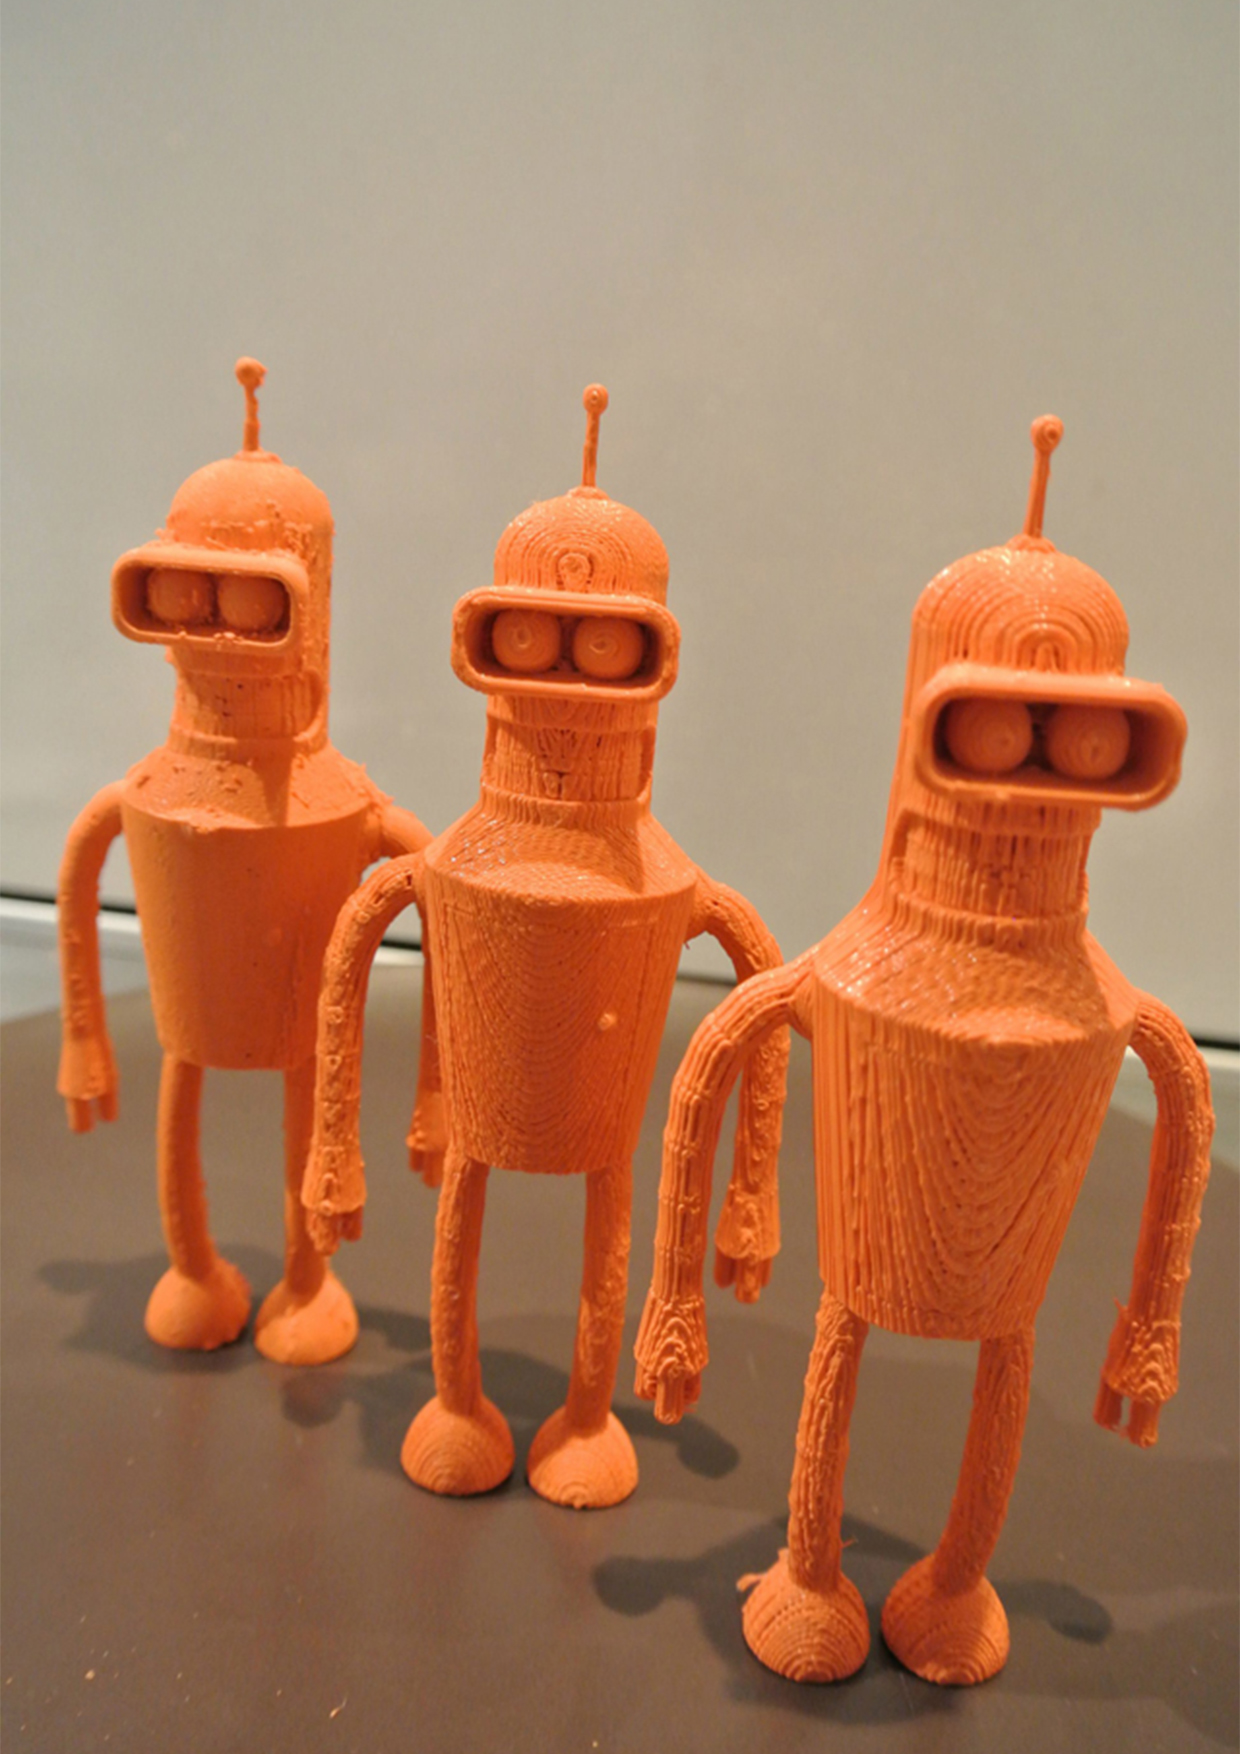
\includepdf{/Users/matthieulapeyre/Documents/phd_thesis/media/3DprintedBlender.pdf}

\chapter{The open hardware and 3D printing revolution} % (fold)



\section{Introduction} % (fold)

The last decades, thanks to the democratization of personal computers and the development of Internet, computer science has known a great expansion.  Open source software played a major role in this expansion. Indeed, most of the web sever are running under open source operating system (Linux) while open source software ...
While copying bits of a software is virtually free, producing the atoms of a hardware has a cost.
Meanwhile the production of both mechanic or electronics hardware components  was limited to two options. Either it was handcrafted or mass produced. Indeed production in small or medium series are extremely difficult to achieve. Conventional manufacturing processes require the production of specific tools, the programming of complex machine, the human intervention to put the part along the different tool etc ... Mosts of the cost are in the up-front tooling, and the more complicated a product is, the more it costs. Thus, most of companies will not accept to run a whole production process just for few units and if they accept the cost will be so high than most prototypes never find a way to reach people outside the workshop they had been created. Only big companies were able to raise enough money to produce new hardware and the niche products and personalization were left aside.

These limitations are going to change. First, new economical model are raising based on crowd-funding allowing inventor to get the fundings needed to make their idea produced.

standardisation

consomery goods

But the rules are currently changing. Rapid prototyping is under democratization ans give access to a Low Cost production to everyone.
It is the makers revolution which is predicted to deeply change the economical model of things.
The early adopter of this new tools are called "makers".

This will lead to the emergence of small batch product and variability. From variabilty come the innovation (Pick) and


Need:

Problems associated to hardware diffusion are not specific to commercial products. In scientific research and especially in the robotics field, the production of prototype is a major issue. The same production problem occur.

While

These problems occuring in the inventor/entrepreneur world are also the case in research.

The same problem occurs in the research community. We produce prototype, we need to explore design we do not know how it will works because it is under research.
Acroban was a perfect example, some very good idea such as a multi-articulated column but a realisation handcrafted leading to an impossibility to share our research.

In this chapter, we will discuss the emergence of new production tools also coming with new user behavior under the DIY, makers and open

While open source software project contributed to some major innovation in the building of internet. The open hardware was limited by its

Open source had a major role on the software innovation.

Open soft a montré des choses.
Open hardware est un vieu truc mais qui reste limité
arrivé de method de RP efficace et low cost
Arrivée d'arduino

de plus en plus de tools open source pour créer de nouveaux tools.


The open hardware and 3D printing revolution ( arduino, les imprimantes 3D, les fablabs, de nouvelles façons de créer/produire)

\section{Open source hardware} % (fold)

\subsection{History} % (fold)
- Machine à soie de Lyon.

- Homebrew computing club
% ref( http://en.wikipedia.org/wiki/Homebrew_Computer_Club, http://www.atariarchives.org/deli/homebrew_and_how_the_apple.php)


\subsubsection{Open Hardware definition} % (fold)

\begin{figure}[]
    \begin{center}
        
\includegraphics[height=5cm]{oshw-logo.pdf}
    \end{center}
    \caption{The open source hardware logo}
    \label{fig:ohw-logo}
\end{figure}

\begin{quotation}
  \emph{Open source hardware is hardware whose design is made publicly available so that anyone can study, modify, distribute, make, and sell the design or hardware based on that design. The hardware’s source, the design from which it is made, is available in the preferred format for making modifications to it. Ideally, open source hardware uses readily-available components and materials, standard processes, open infrastructure, unrestricted content, and open-source design tools to maximize the ability of individuals to make and use hardware. Open source hardware gives people the freedom to control their technology while sharing knowledge and encouraging commerce through the open exchange of designs.}

  -- \textbf{Open Source Hardware Association (OSHW)}
\end{quotation}


\subsection{Open source licenses for hardware} % (fold)



Apache, MIT License, GPL, BSD
\subsubsection{Creative Commons licenses} % (fold)


http://creativecommons.org/science

http://creativecommons.org/about/downloads
\begin{NFfigure}
    \begin{center}
        
\includegraphics[height=2cm]{cc-logo.pdf}
    \end{center}
    \caption{Creative Commons logo}
    \label{fig:cc-logo}
\end{NFfigure}

The Creative Commons licenses are based on four major condition modules:
\begin{description}
    \item[BY] Attribution: requiring attribution to the original author.
    \item[NC] Non Commercial: requiring the work is not used for commercial purposes
    \item[ND] No Derivative works: allowing only the original work, without derivatives
    \item[SA] Share Alike: allowing derivative works under the same or a similar license (later or jurisdiction version).
\end{description}


The combination of these modules leads to six licenses.

\begin{description}
    \item[] 
\includegraphics[width=2.5cm]{cc-by.pdf} \\ \textbf{Attribution CC BY} People can distribute, remix, tweak and build upon the licensed work, even commercially, as long as they credit the authors of the original creation.
    \item[Attribution-ShareAlike CC BY-SA] \begin{center} 
\includegraphics[width=2.5cm]{cc-by-sa.pdf} \end{center} People can distribute, remix, tweak and build upon the licensed work, even commercially, as long as they credit the authors and license their new creations under the identical terms. \textbf{This license is often compared to “copyleft” free and open source software licenses.}
    \item[Attribution-NoDerivs CC BY-ND] \begin{center} 
\includegraphics[width=2.5cm]{cc-by-nd.pdf} \end{center} This license allows for redistribution, commercial and non-commercial, as long as it is passed along unchanged and in whole, with credit to the authors.
    \item[Attribution-NonCommercial CC BY-NC] \begin{center} 
\includegraphics[width=2.5cm]{cc-by-nc.pdf} \end{center} This license lets people remix, tweak, and build upon the work for non-commercial purpose. Although their new works must also acknowledge the original authors and be non-commercial, they do not have to license their derivative works on the same terms.
    \item[Attribution-NonCommercial-ShareAlike CC BY-NC-SA] \begin{center} 
\includegraphics[width=2.5cm]{cc-by-nc-sa.pdf} \end{center} This license lets people remix, tweak, and build upon the work for non-commercial purpose, as long as they credit the authors and license their new creations under the identical terms.
    \item[Attribution-NonCommercial-NoDerivs CC BY-NC-ND] \begin{center} 
\includegraphics[width=2.5cm]{cc-by-nc-nd.pdf} \end{center} This license is the most restrictive of the six main Creative Commons licenses, only allowing people to download the works and share them with others as long as they credit the authors, but they cannot change them in any way or use them commercially.
\end{description}


\subsection{A growing movement} % (fold)



\begin{figure}[H!]
    \begin{center}
        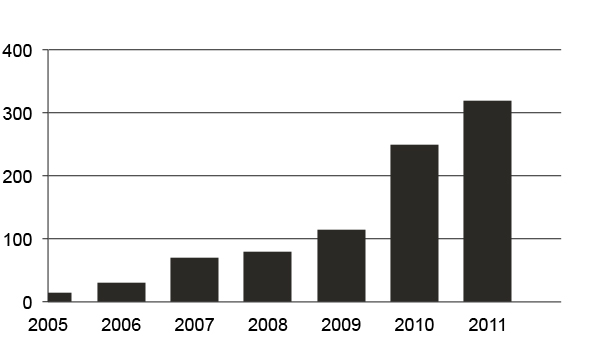
\includegraphics[height=8cm]{oh_project_evolution.jpg}
    \end{center}
    \caption{Creation of new open hardware project per year between 2005 and 2011. Graphic extracted from \emph{HOPE 2010 - How to run an open source hardware company}}
    \label{fig:oh_project_evolution}
\end{figure}


\begin{figure}[]
    \begin{center}
        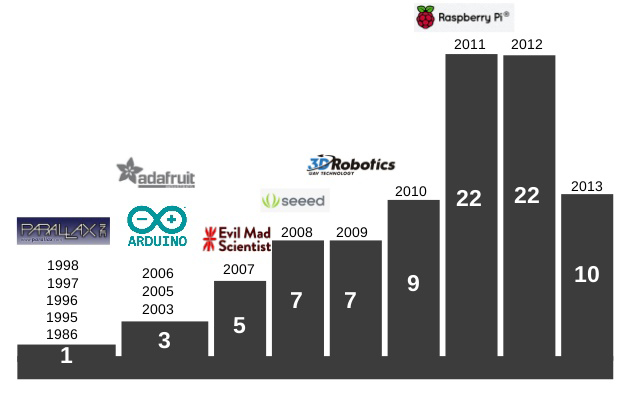
\includegraphics[height=8cm]{oh_startup_creation.jpg}
    \end{center}
    \caption{Start-up creation based on open hardware distribution}
    \label{fig:oh_startup_creation}
\end{figure}

\subsection{Famous projects} % (fold)



\subsubsection{Arduino} % (fold)

Started in 2005, the Arduino project aimed to offer an affordable and easy to use electronics board for students. Back at this time, students from the Interaction Design Institute Ivrea in Italy were using \emph{BASIC Stamp}\footnote{A BASIC Stamp module is a single-board computer that runs the Parallax PBASIC language interpreter in its microcontroller.} at a cost of \$100.

\begin{NFfigure}
    \begin{center}
        
\includegraphics[height=3cm]{arduino_logo.png}
    \caption{The Arduino logo}
    \label{fig:arduino_logo}
    \end{center}
\end{NFfigure}

To make the board, the development team had a specific, student-friendly price as their goal: \$30. \emph{It had to be the equivalent of going out to dinner at a pizza place}, Banzi said \footnote{David Kushner (26 Oct 2011). \emph{The Making of Arduino}. IEEE Spectrum.}.

A hardware thesis by Hernando Barragan\cite{barragan2004wiring} was contributed for a wiring design. After the wiring platform was complete, researchers worked to make it lighter, less expensive, and available to the open source community. The open-source model had long been used to fuel innovation for software, but not hardware. To make it work, they had to find an appropriate licensing solution that could apply to their board. After some investigation, they realized that if they simply looked at their project differently, they could use a license from Creative Commons, the nonprofit group whose agreements are normally used for cultural works such as music and writing. \emph{You could think of hardware as piece of culture you want to share with other people}, Banzi said.

Arduino is a platform for prototyping interactive objects using electronics. It consists of both hardware and software: a circuit board that can be purchased at low cost or assembled from freely-available plans; and an open-source development environment and library for writing code to control the board. Arduino comes from a philosophy of learning by doing and strives to make it easy to work directly with the medium of interactivity. It extends the principles of open source to the realm of hardware, supporting a community of people working with and extending the platform. It has been used in universities around the world and in numerous works of interactive art.\cite{mellis2007arduino}



\subsubsection{Raspberry Pi} % (fold)
% \begin{row}{4}{2}
%     \begin{cell}{3}
%     The Raspberry Pi is a credit-card-sized single-board computer developed in the UK by the Raspberry Pi Foundation with the intention of promoting the teaching of basic computer science in schools.
%     \end{cell}
%     \begin{cell}{1}
%     \begin{NFfigure}
%     \begin{center}
%         
\includegraphics[height=3cm]{raspberry_pi_logo.png}
%     \end{center}
%     \caption{The Raspeberry Pi logo}
%     \label{fig:raspberry_pi_logo}
% \end{NFfigure}
%     \end{cell}
% \end{row}




\begin{NFfigure}
    \begin{center}
        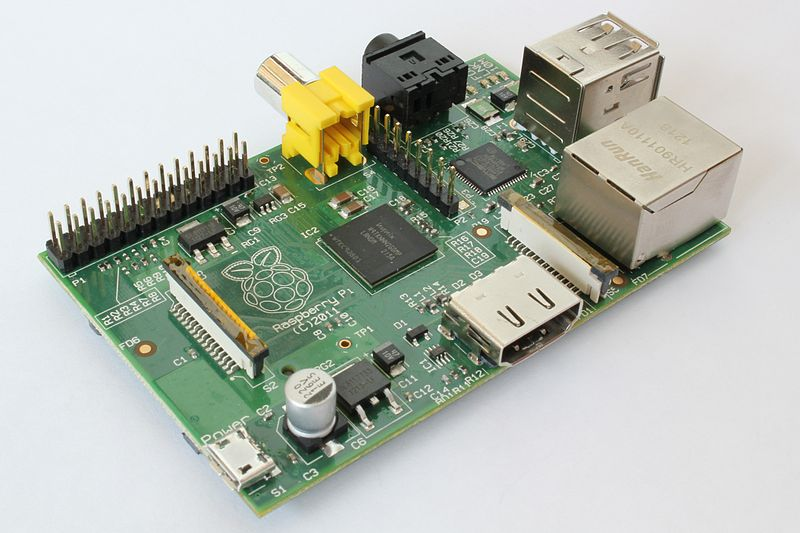
\includegraphics[height=5cm]{raspberry_pi.jpg}
    \end{center}
    \caption{The Raspeberry Pi board}
    \label{fig:raspberry_pi}
\end{NFfigure}

\subsubsection{Shapeoko} % (fold)

\begin{NFfigure}
    \begin{center}
        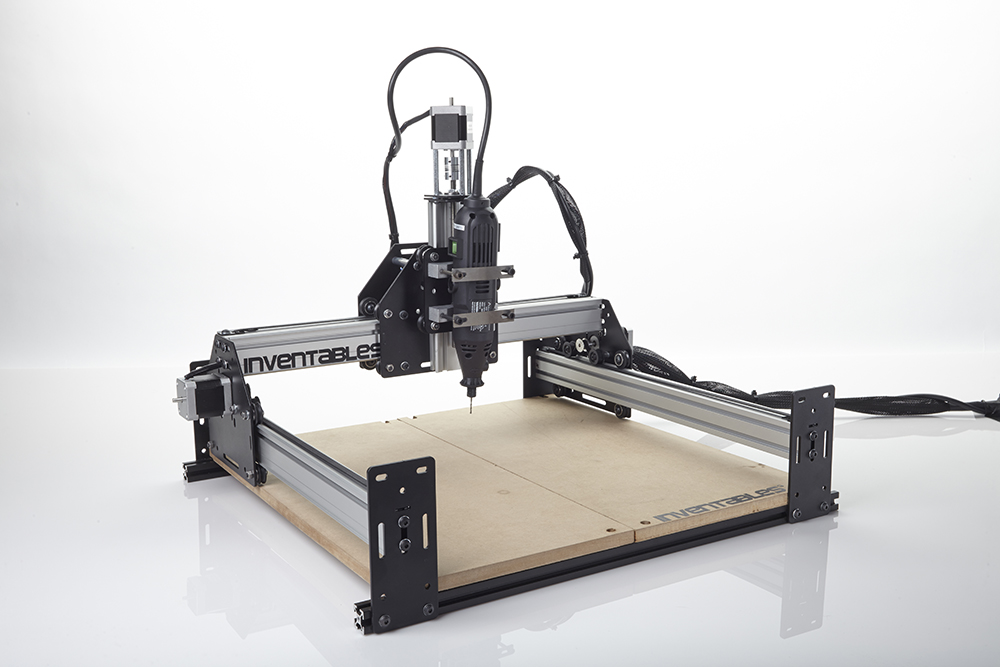
\includegraphics[height=5cm]{shapeoko_v2.jpg}
    \end{center}
    \caption{Caption here}
    \label{fig:shapeoko_v2}
\end{NFfigure}

\subsubsection{RepRap} % (fold)

The RepRap project was the first low cost 3D printer.
\begin{quotation}
RepRap takes the form of a free desktop 3D printer capable of printing plastic objects. Since many parts of RepRap are made from plastic and RepRap prints those parts, RepRap self-replicates by making a kit of itself - a kit that anyone can assemble given time and materials. It also means that - if you've got a RepRap - you can print lots of useful stuff, and you can print another RepRap for a friend...
\end{quotation}


\begin{NFfigure}
    \begin{center}
        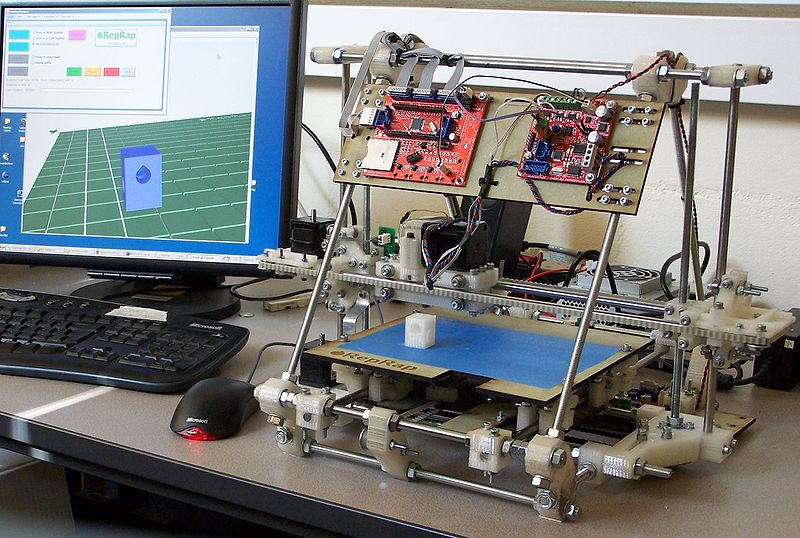
\includegraphics[height=5cm]{RepRap_v2.jpg}
    \end{center}
    \caption{Caption here}
    \label{fig:RepRap_v2}
\end{NFfigure}


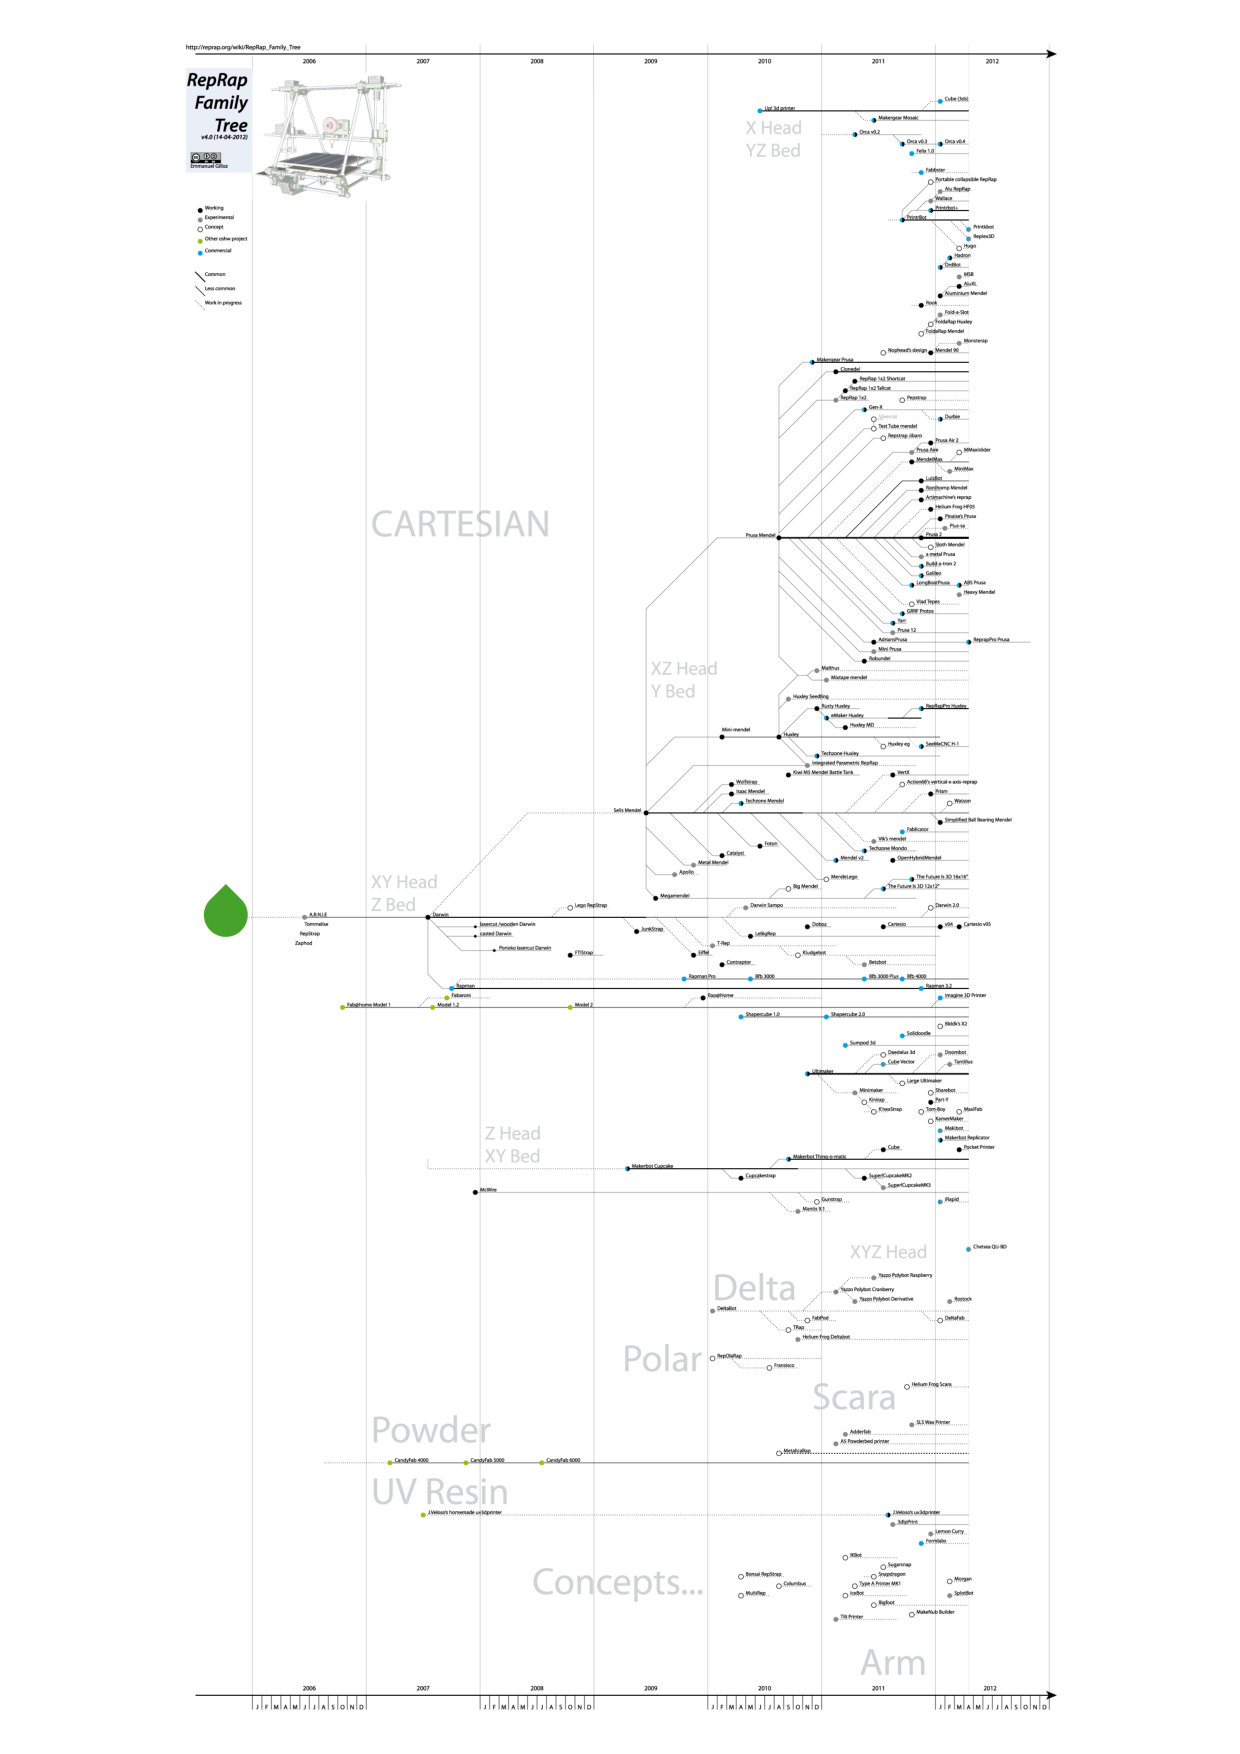
\includepdf{/Users/matthieulapeyre/Documents/phd_thesis/media/open_hardware/reprap_family_tree.pdf}

\begin{figure}[]
    \begin{center}
        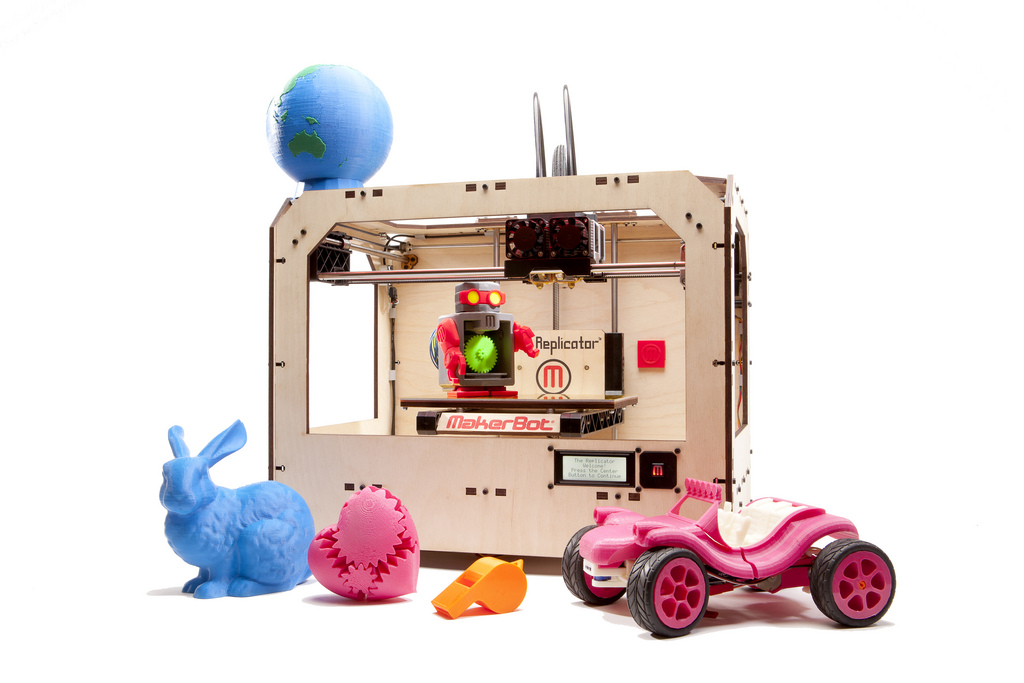
\includegraphics[height=8cm]{makerbot-replicator.jpg}
    \end{center}
    \caption{Caption here}
    \label{fig:makerbot-replicator}
\end{figure}

the ikea effect

Von Hippel, Eric (2002) "Shifting Innovation to Users via Toolkits", Management Science Vol 48, No 7, July
 Von Hippel, Eric (1986) Lead Users: A source of Novel Product Concepts. Management Science. Vol 32, No 7,
July 1986

Von Hippel, Eric (1994). " Sticky Information and the locus of problem solving: Implications for innovation."
Management Science, 40(4) 429-439

http://www.ohanda.org/


\section{Rapid prototyping} % (fold)

\paragraph{A comparison of rapid prototyping technologies (Pham 1997)}

"Prototyping is an essential part of the product development and manugacturing cycle required for assessing the forim, fit and functionality of a design before a significant investment in tooling is made. Until recently, prototypes were largerly handmade by skilled craftsmen, adding weeks or months to the product development time. Because of this, only a few design iterations could be made before tooling went into production, resulting in parts which at best were seldom optimised and at worst did not function properly.
Rapid Prototyping is a term which embraces a range of new technologies for producing accurate parts directly from CAD models in a few hours, with littel need for human intervention. This means that desigenrs have the freedom to produce physical models of theirs drawings more frequently, allowing them to check the assembly and function of the design as well as discussing downstream manufacturing issues with an easy-to-interpret, unambigous prototype. Consequently, errors are minimised and product development costs and lead times substantially reduced. It has been claimed that rapid proto can cut new product costs by up to 70\% and the time to market by 90\%."
- Rapid product development in the USA, Europe and Japan (Waterman 1994)


\subsection{Several technologies} % (fold)

\subsubsection{Stereolithography (SL)} % (fold)

This relies on a photosensitive monomer resin which forms a polymer and solidifies when exposed to ultraviolet (UV) light. Due to the absorption and scattering of the beam this reaction only takes place near the surface.

Y'en a plein dans A comparison of rapid prototyping technologies (Pham 1997)

\subsubsection{Selective laser sintering} % (fold)
SLS uses a fine powder which is heated with a CO2 laser of power in the range of 25-50W such that the surface tensions of the grains are overcome and they fuse together.Before the powder is sintered, the entire bed is headted to just below the melting point of the material in order to minimize thermal distortion and facilitate fusion to the previous layer.

\subsubsection{Filament} % (fold)




\subsection{Introduction} % (fold)

Production process by material addition.



\section{Makers \& Fablab: } % (fold)

http://alternatives.blog.lemonde.fr/2014/04/06/ces-projets-open-source-qui-changent-le-monde/



http://www.gizmag.com/disney-research-3d-printed-optics/24435/
http://www.3ders.org/articles/20131119-first-ever-3d-printed-electronics-set-to-launch-into-space-today.html


% \cleartoleftpage
% \part{The Poppy project} % (fold)
% The Poppy project aims to ...
% !TEX root = ../../thesis.tex

\chapter{Motivations and Methodology}
\label{cha:methodology}

\section{Introduction} % (fold)

In chapter~\ref{cha:morphology-review}, we discussed the emergence of a novel paradigm in the field of robotics that appeared in the late eighties.  Embodied artificial intelligence rejects the symbolic approach and postulates that it is not possible to have intelligence without an actual robot body associated with its ecological niche~\parencite{pfeifer2001understanding}. Following this paradigm, several researchers have tried to tackle challenges in which the classical cognitivist approach failed (see \parencite{brooks1986achieving}) e.g. the understanding of natural forms of intelligence that require direct interaction with the real world.

Thus, an interesting evolution over recent decades is the demonstration of the importance of the morphology for sensorimotor control, cognition and development (\parencite{kaplan2008corps} \parencite{steels1995artificial} \parencite{Pfeifer06}), which can be defined as follows:
\begin{formal}
    The morphology of a robot thus refers to the physical structure and form of a robot. Specifically, the focus is on characteristics such as link sizes, number of links, joint characteristics, mass distribution, actuator characteristics, material properties, sensor characteristics and sensor placements. In short, any characteristic that defines the physical structure of the robot is included in the term morphology.
    \signed{Chandana Paul~\parencite{paul2006morphological}}
\end{formal}

Exploring the interaction between body properties and cognition could lead both to a better understanding of animals’ behaviour (human beings in particular) and to build robots that are more adapted and robust to an open environment with unpredictable interactions. In particular, we can highlight the acquisition of sensorimotor tasks and the exploration of adapted bodies for natural, physical and social interactions with humans.

In this context, we should not only pay attention to the robot body design but \textbf{introduce morphology as an experimental variable and conduct experiments in the real world}. As Rodney Brooks said \emph{the world is its own best model}~\parencite{brooks1991intelligence} and simulators cannot handle the complexity of real physics with multi-point contacts, soft materials and frictions. This is especially true for complex dynamic tasks such as physical interaction or legged locomotion.

Following the definition of robotic morphology given by C. Paul, we need to find a framework allowing easy and quick tuning of morphological parameters on an actual robot in order to explore and hopefully find new ways of improving robot behaviour in the real world. However considering morphology as an experimental variable raised two major problems:
\begin{itemize}
    \item \textbf{how can we obtain an experimental robotic platform with both a morphology that can be changed easily and quickly and the capacity to act robustly in the real world? }
    \item \textbf{how can we make sure this platform, particularly the hardware,  can be diffused and reused in the research community?}
\end{itemize}

In the next sections of this chapter, we will \textbf{suggest novel approaches and design processes to create and produce robotic platforms,  the control and morphology of which can be freely explored through experimentation in the real world,  that are easy to  diffuse and reproduce in the research community.}
We will detail the methodological and design challenges involved in creating robots with variable and modular hardware. Then we will present the design methods we chose to address these challenges and those we have used to create Poppy (see chapter REF). And finally, we will discuss the importance of open source distribution for creating open and cumulative science.


\section{Challenges} % (fold)

The role of morphology appears to be a fascinating open field of research but until now it has been under-explored.
We presented in chapter~\ref{cha:experimental-methods}, a review of robotic platforms, both commercial and lab prototypes. It appears the current platforms are not suitable to tackle these challenges.

Firstly, for most the electronic and mechanical structures are produced using classic manufacturing techniques,  which makes them too complicated and expensive to modify. Indeed, the classical way of designing and producing robots is a complicated, time-consuming and expensive process. The development of current robotic platforms requires dozens of engineers working for many years and significant fund-raising for production. Such techniques make creating variant parts impossible, mainly because of the approach and technologies chosen to design and produce them.


Secondly, beyond the restriction on exploring morphological variants, one of the fundamental aspects of the scientific research is to demonstrate facts, which should therefore be reproducible. Unfortunately in the robotics field, the amount of material resources and the techniques involved makes it difficult to transfer robot platforms from one lab to another. While commercial robots can be easily accessible (subject to appropriate funding) because they are relatively mass-produced, lab prototypes are mainly handcrafted and specifically tuned, which makes their  reproduction in another lab impossible. Therefore, scientific validation is limited and researchers cannot build novel work upon that of their peers.

Finally, robot hardware of both types is very rarely open source, which simply prohibits any modification and reuse of the work (we will discuss more in detail the importance of this point in section REF).

Therefore, allowing  experimental platforms to be transferred and shared is a way of ensuring the scientific validity of experiments, and also of promoting and accelerating scientific research by reducing time lost in development, instead concentrating research resources on the exploration of novel ideas.


In this context, creating a platform reproducible everywhere without special tooling or skills, the morphology of which can be freely explored, raises methodological and design process challenges that we will describe in the following points.

\subsection{Make the morphology variable} % (fold)

Current robotic platforms, in particular humanoid ones, have mechanical parts either handcrafted or produced with classic machining techniques based on milling or casting metal alloys or plastic.
These techniques require specific upfront tooling which make the production of a small batch really expensive. Also, to keep the cost of the robot rather low, mass production is needed to achieve economy of scale. In this context, the morphology of current robotic platforms cannot be modified because it would require redoing most of the production process. In addition, the design of such mechanical parts is limited because the manufacturing process implies constraints and the complexity of a part greatly increases its cost. The same issues appear with electronics and the robot sensor space which is, in most cases, frozen. Thus the classic way to design and produce robot is not adapted to the free exploration of the robot morphology, novel design and production paradigm have to be used.


\subsection{Create reproducible robot prototypes} % (fold)

Most labs must reinvent the wheel by developing whole new robotic platforms even though functional setups have already been developeded by other laboratories and could be reused.

For example, several interesting robotic platforms explore key aspects of robot morphology. We can cite Kenshiro~\parencite{nakanishi2013design} which has a complex and bio-inspired artificial muscles actuator network, or semi-passive walkers such as Denise~\parencite{wisse2005three}, demonstrating impressive walking ability with little control and power actuation. Unfortunately, none of these robots can be and have ever been transferred to another lab. Indeed even if they were open source theirs productions require specific tooling and hand tuning that only few skilled people have.

Therefore some constraints have to be applied on hardware platforms to make them reproducible:
\begin{description}
    \item[Precision, stationary] Experiments should be repeatable, implying that the robot’s morphological properties should be stationary. This means that robot performance should not be dependent on where it was built or the users’ skills.
    \item[Easy and fast to duplicate:] In order for the platform to be reusable, it needs to be easy and fast to duplicate and not rely on specific tooling or exotic components.
    \item[Affordable:] To ensure widespread use, a key aspect is to keep the cost of the platform relatively low. The more labs involved, the better the scientific impact.
\end{description}


\subsection{Keep robotic platform simple and easy-to-use} % (fold)

The field of robotics is intrinsically multidisciplinary. A robot itself requires technology from mechanics, electronics and computer science, but the scientific impact of robotics can be far larger and reach non-engineering fields such as human, social or biological sciences. Thus, robotics is a specialised field  in which nobody can be an expert in all required skills.
We have to take into account the fact that the end user can certainly be expert in one specific subfield but a beginner in others. This mean that for each subfield, the designed robot has to be simple enough to be understood and used by beginners while having, at the same time, enough potential to not constrain users in their domain of expertise.



\section{The chosen design methods} % (fold)

To address these challenges, we suggest exploring an alternative design methodology that is driven by the desire to:
\begin{itemize}
    \item freely explore morphological properties,
    \item reduce the amount of time required between an idea and its experimentation on an actual robotic platform in the real world,
    \item make our work easily reproducible in any other lab,
    \item keep our work modular and free to use in accordance with open source principles, so it can be reused and extended for other projects.
\end{itemize}


To reach these goals, we decided to follow some design methods for both design and production, for all technological aspects of the robot (i.e. mechanics, actuation, electronics, software, distribution).

\subsection{3D-printed mechanical parts} % (fold)
We could envisage simply having classical mechanical parts that are reconfigurable and adjustable, allowing for example, the exploration of different lengths of a link or different centre of mass positions. However, this limits the morphological exploration to only a few dimensions with a limited range.

As we discussed in chapter REF, over the last few years, novel techniques, especially 3D printing have been revolutionizing the way we can produce objects. 3D printers not only open new horizons for the production of mechanical part, they are able to produce parts that were either not possible or extremely expensive with classical techniques (see \figurename~\ref{fig:complex_3D_printed_part}) but also completely change the paradigm associated with production. Indeed the cost does not change with the quantity or the complexity, meaning designers are free to explore the shape they want with almost no constraints.

\begin{figure}[tb]
\centering
    \subfloat[][]{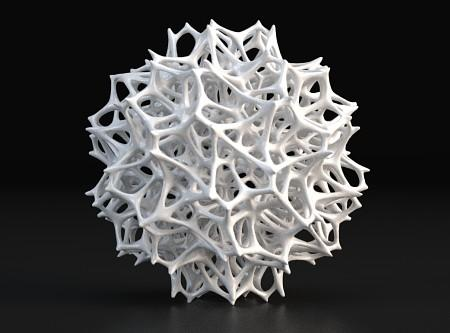
\includegraphics[width=0.4\linewidth]{complex_3Dprinted_part.jpeg}}
    \hfil
    \subfloat[][3D printed metal heat exchanger]{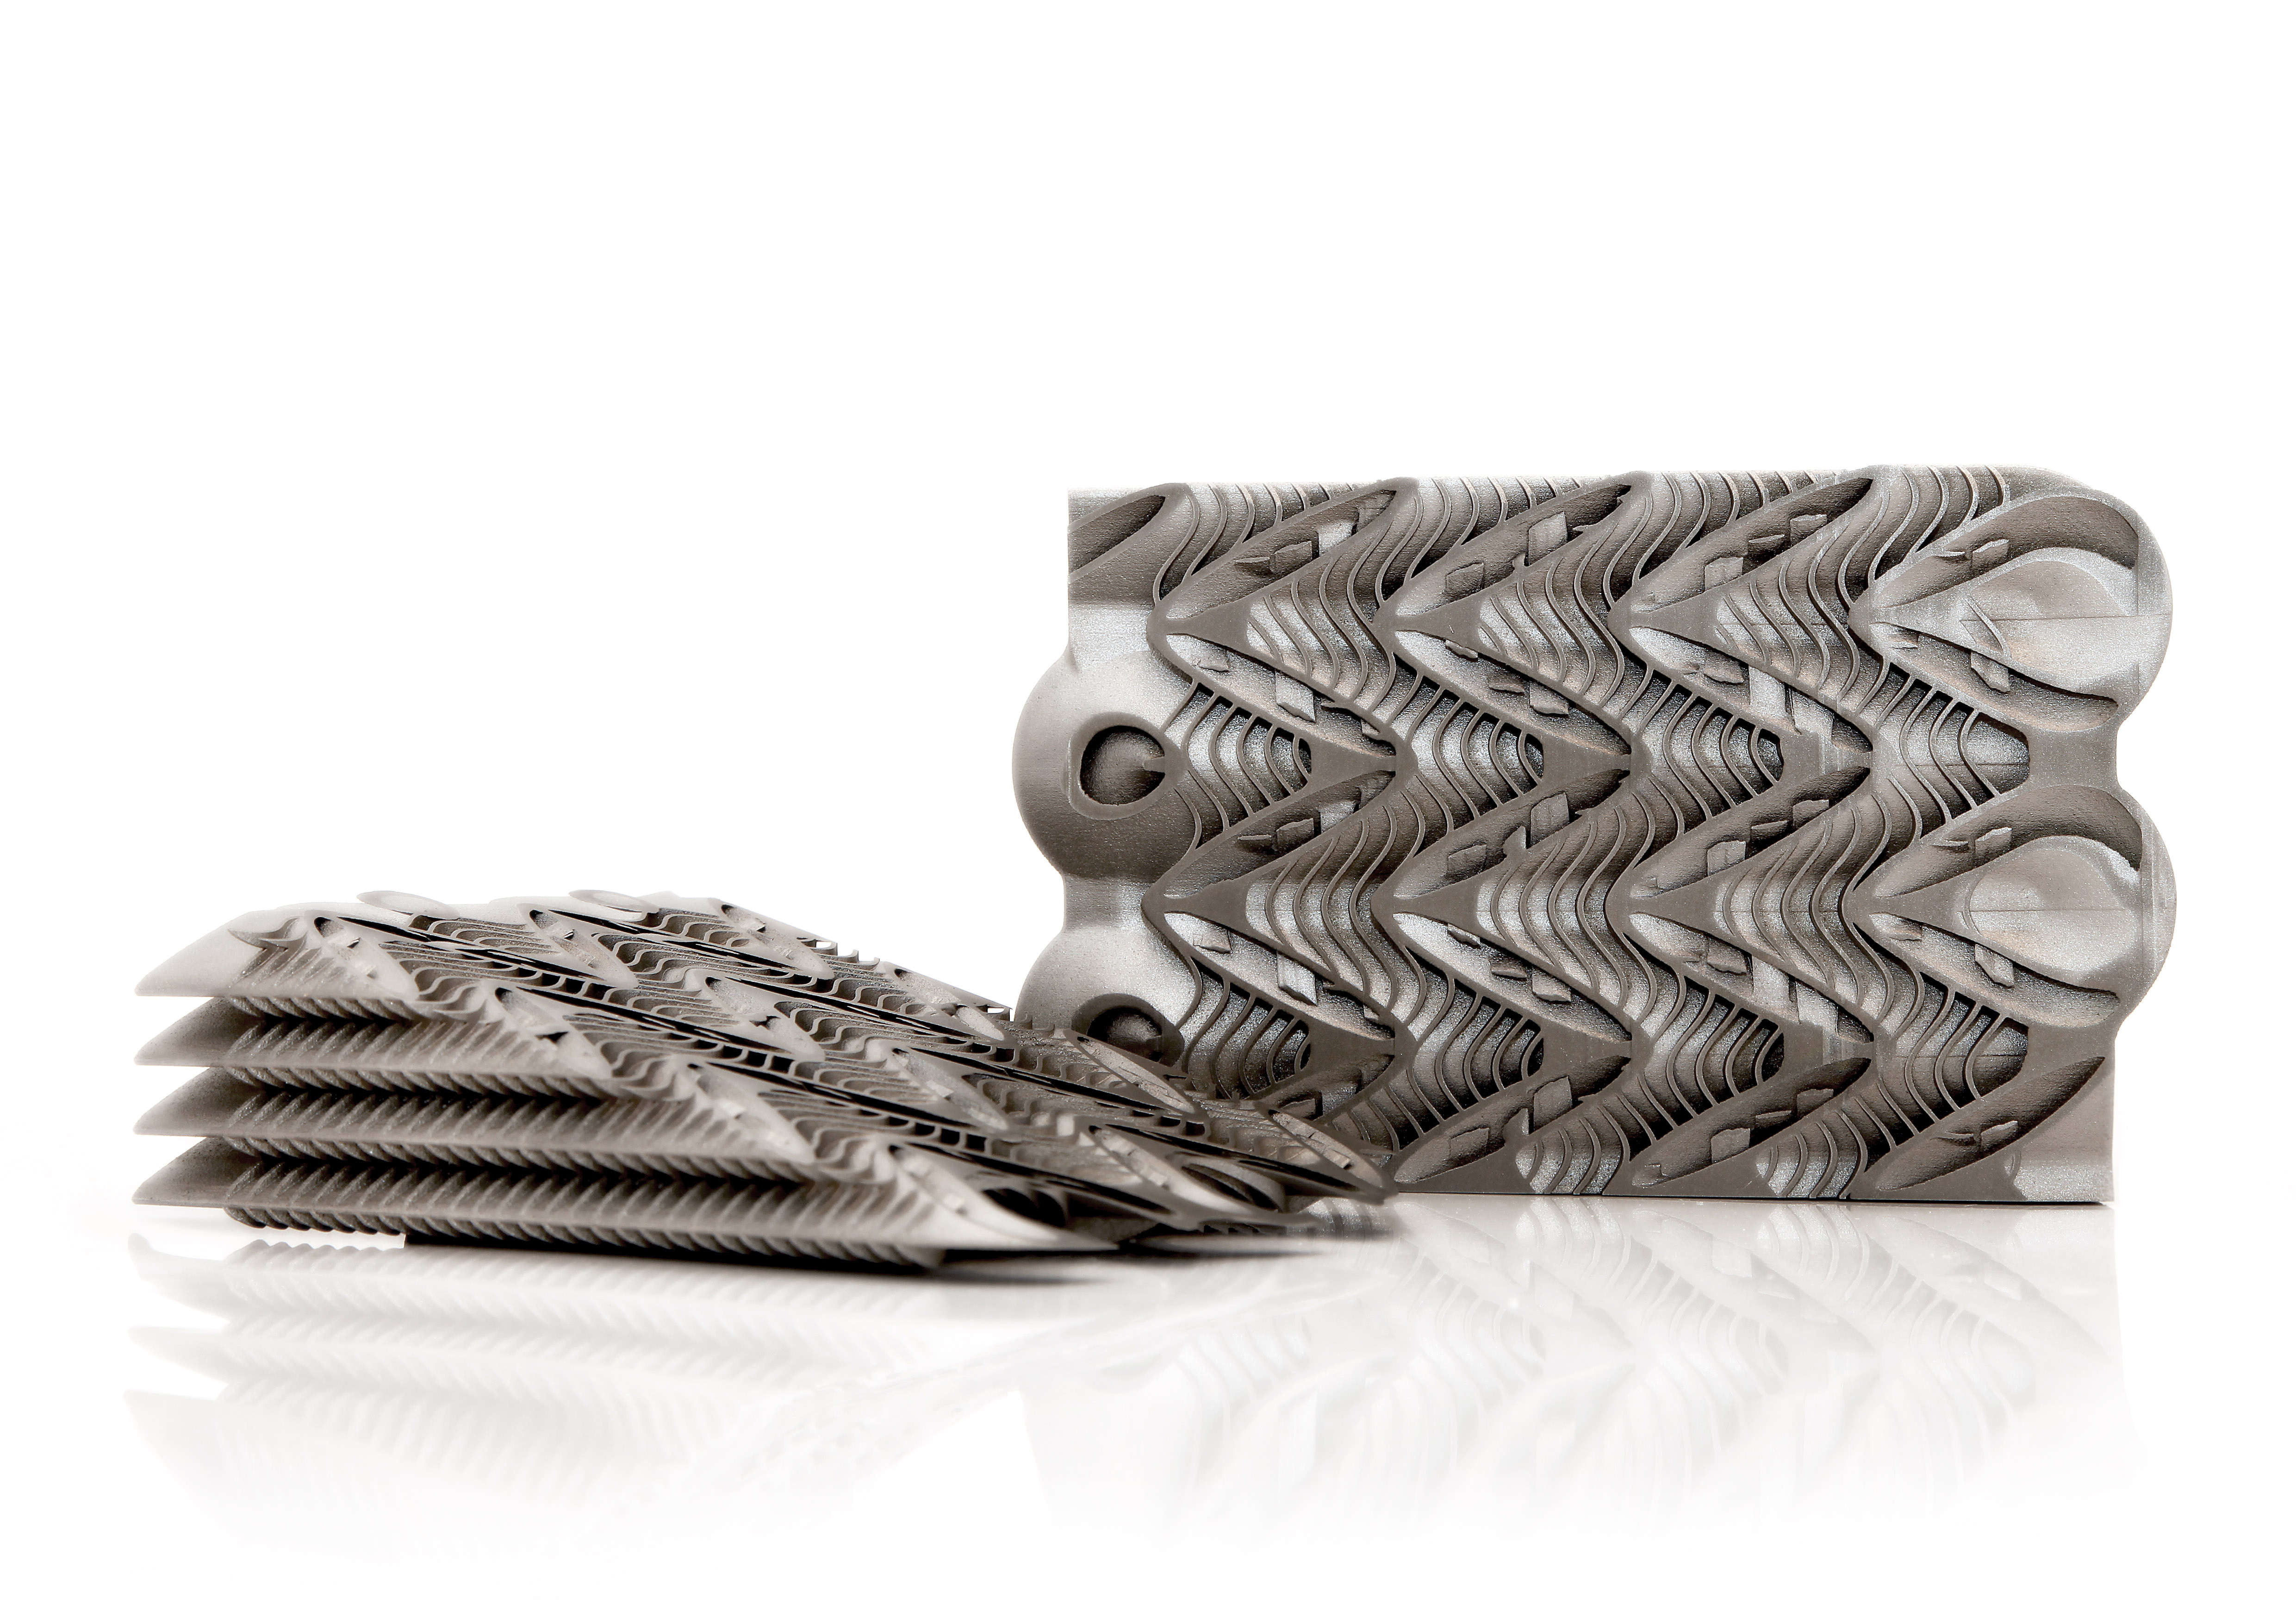
\includegraphics[width=0.55\linewidth]{complex_heat_exchanger.jpg}}
    \caption{}
    \label{fig:complex_3D_printed_part}
\end{figure}


Also, these novel techniques come with the open hardware and makers revolution, which has brought low cost 3D printers into the home. The production of mechanical parts can be now done in few hours directly on site with limited human handling.

\begin{figure}[tb]
    \begin{center}
        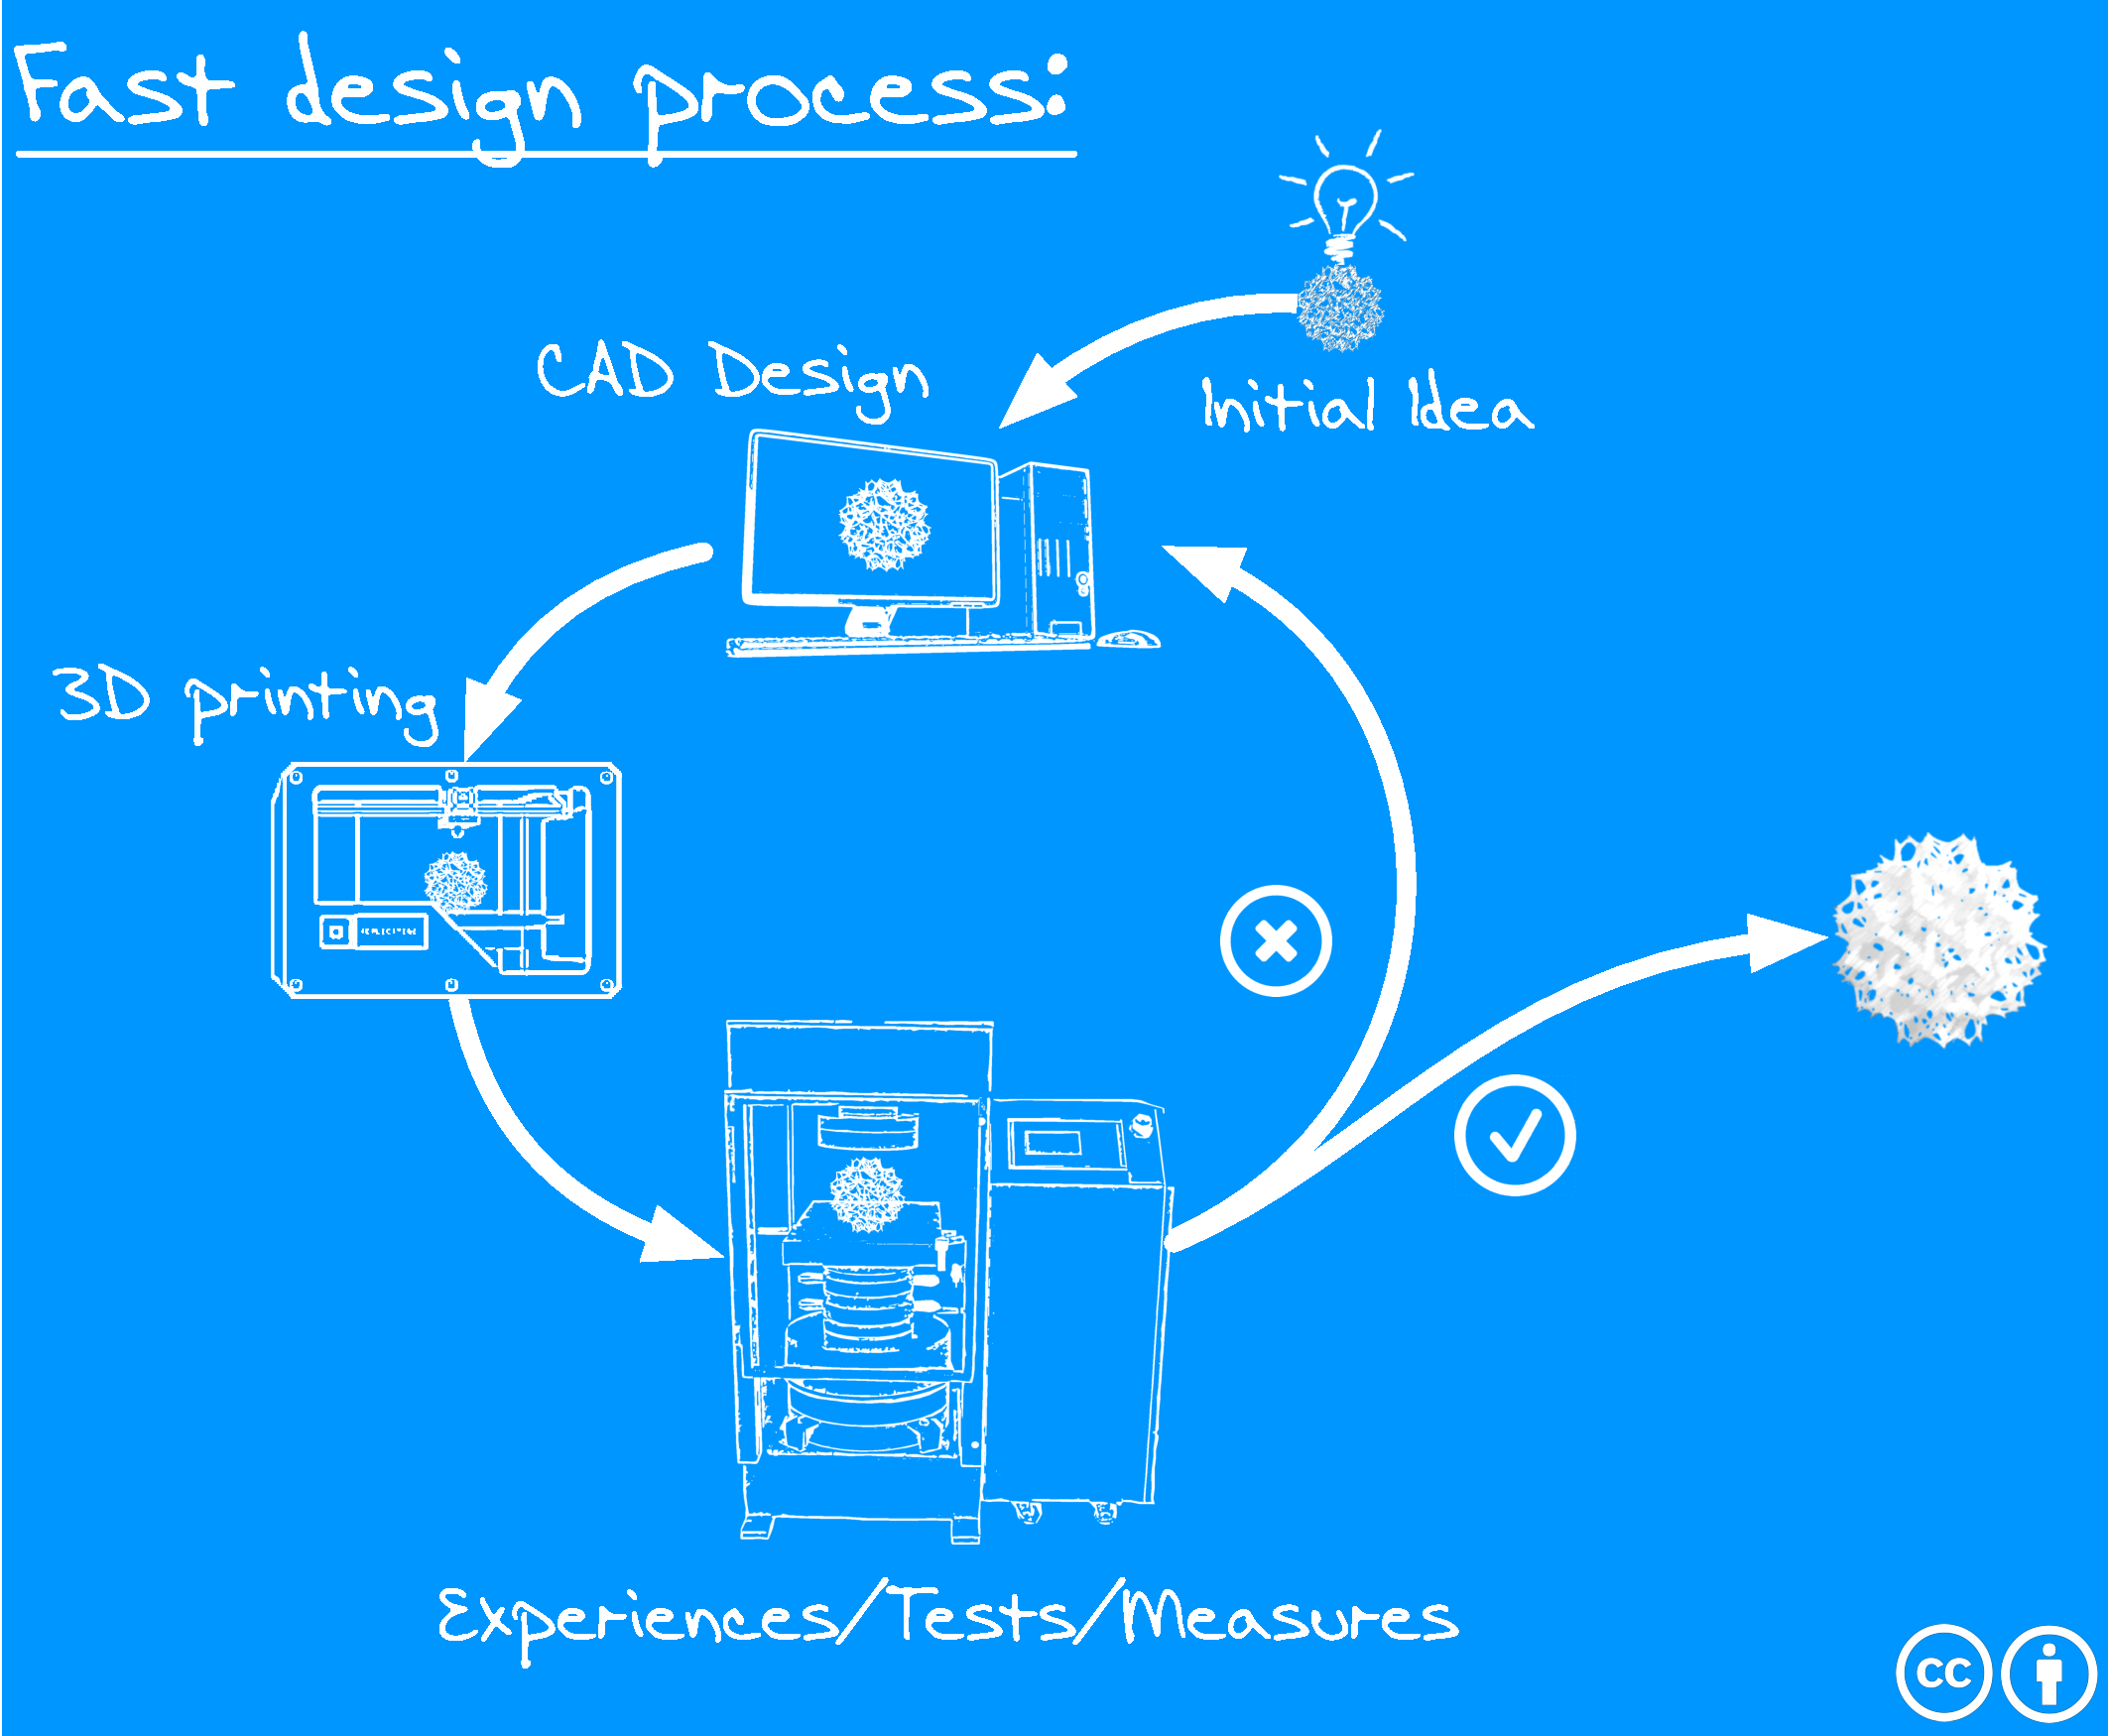
\includegraphics[width=\linewidth]{conception_iterative.pdf}
    \end{center}
    \caption{Fast conception loop}
    \label{fig:conception_loop}
\end{figure}

3D printers have several key abilities:
\begin{description}
    \item[Worldwide:] 3D printed parts can be obtained everywhere, either by personal printing or by ordering parts on other web services, such as i.materialise, shapeways or sclupteo.
    \item[Low cost:] The cost of producing 3D parts is rather low, ranging from tens of cents if produced on a personal printer to tens of euros if ordered though a web service.
    \item[Fast:] In a couple of hours a whole part can be created from scratch. When using web services, queuing and shipping delays have to be added, increasing the production time to several days.
    \item[Skill-free:] Since the production process is fully digital, few or no specialist skills are required.
    \item[Multi-material, precise and robust:] current 3D printers can create precise (up to 0.1mm) parts in different material such as nylon, PLA, ABS or even titanium and flexible material. The parts obtained are robust and can be used as final parts for several years.
    \item[Reduce the number of part:] 3D printing  can be used to print complex parts and even assembled parts as complex as bearings or gearboxes. This means we can replace multiple parts that have to be assembled into ready-to-use ones.
\end{description}

These properties of the 3D printing process allow for the first time to really explore morphological variants of mechanical parts. Indeed, it is now fast and low-cost to create alternative designs. Associated with modular architecture, we can easily and quickly change robot parts and conduct experiments. Also this process is compatible with our diffusion goals since it is simple and accessible anywhere with an internet connection and a mailing address.


\subsection{Electronic architecture based on Arduino} % (fold)

Thanks to 3D printing, exploring morphological variants of mechanical parts is now easier than ever before but unfortunately, the printing of electronic components and boards is not yet available. However, exploring the role of morphology does not only concern the mechanical properties but also the sensors apparatus i.e. \textbf{which sensor is used and where is it placed on the body}. The Swiss bot (see REF) is a great example of the impact of the sensors’ positioning on robot behaviour.

To permit the exploration of sensor-system variants, we suggest basing the electronic architecture on Arduino. Arduino is an open-source electronics platform based on easy-to-use hardware and software. It is intended for anyone doing interactive projects. The Arduino board can sense the environment by receiving inputs from a wide variety of sensors, and affects its surroundings by controlling lights, motors, and other actuators. Low-level embedded programing skills are not required, since Arduino boards can be programmed using the Arduino programming language\footnote{\url{http://arduino.cc/en/Main/Software}} which abstracts all the complexity.

\begin{figure}[tb]
    \begin{center}
        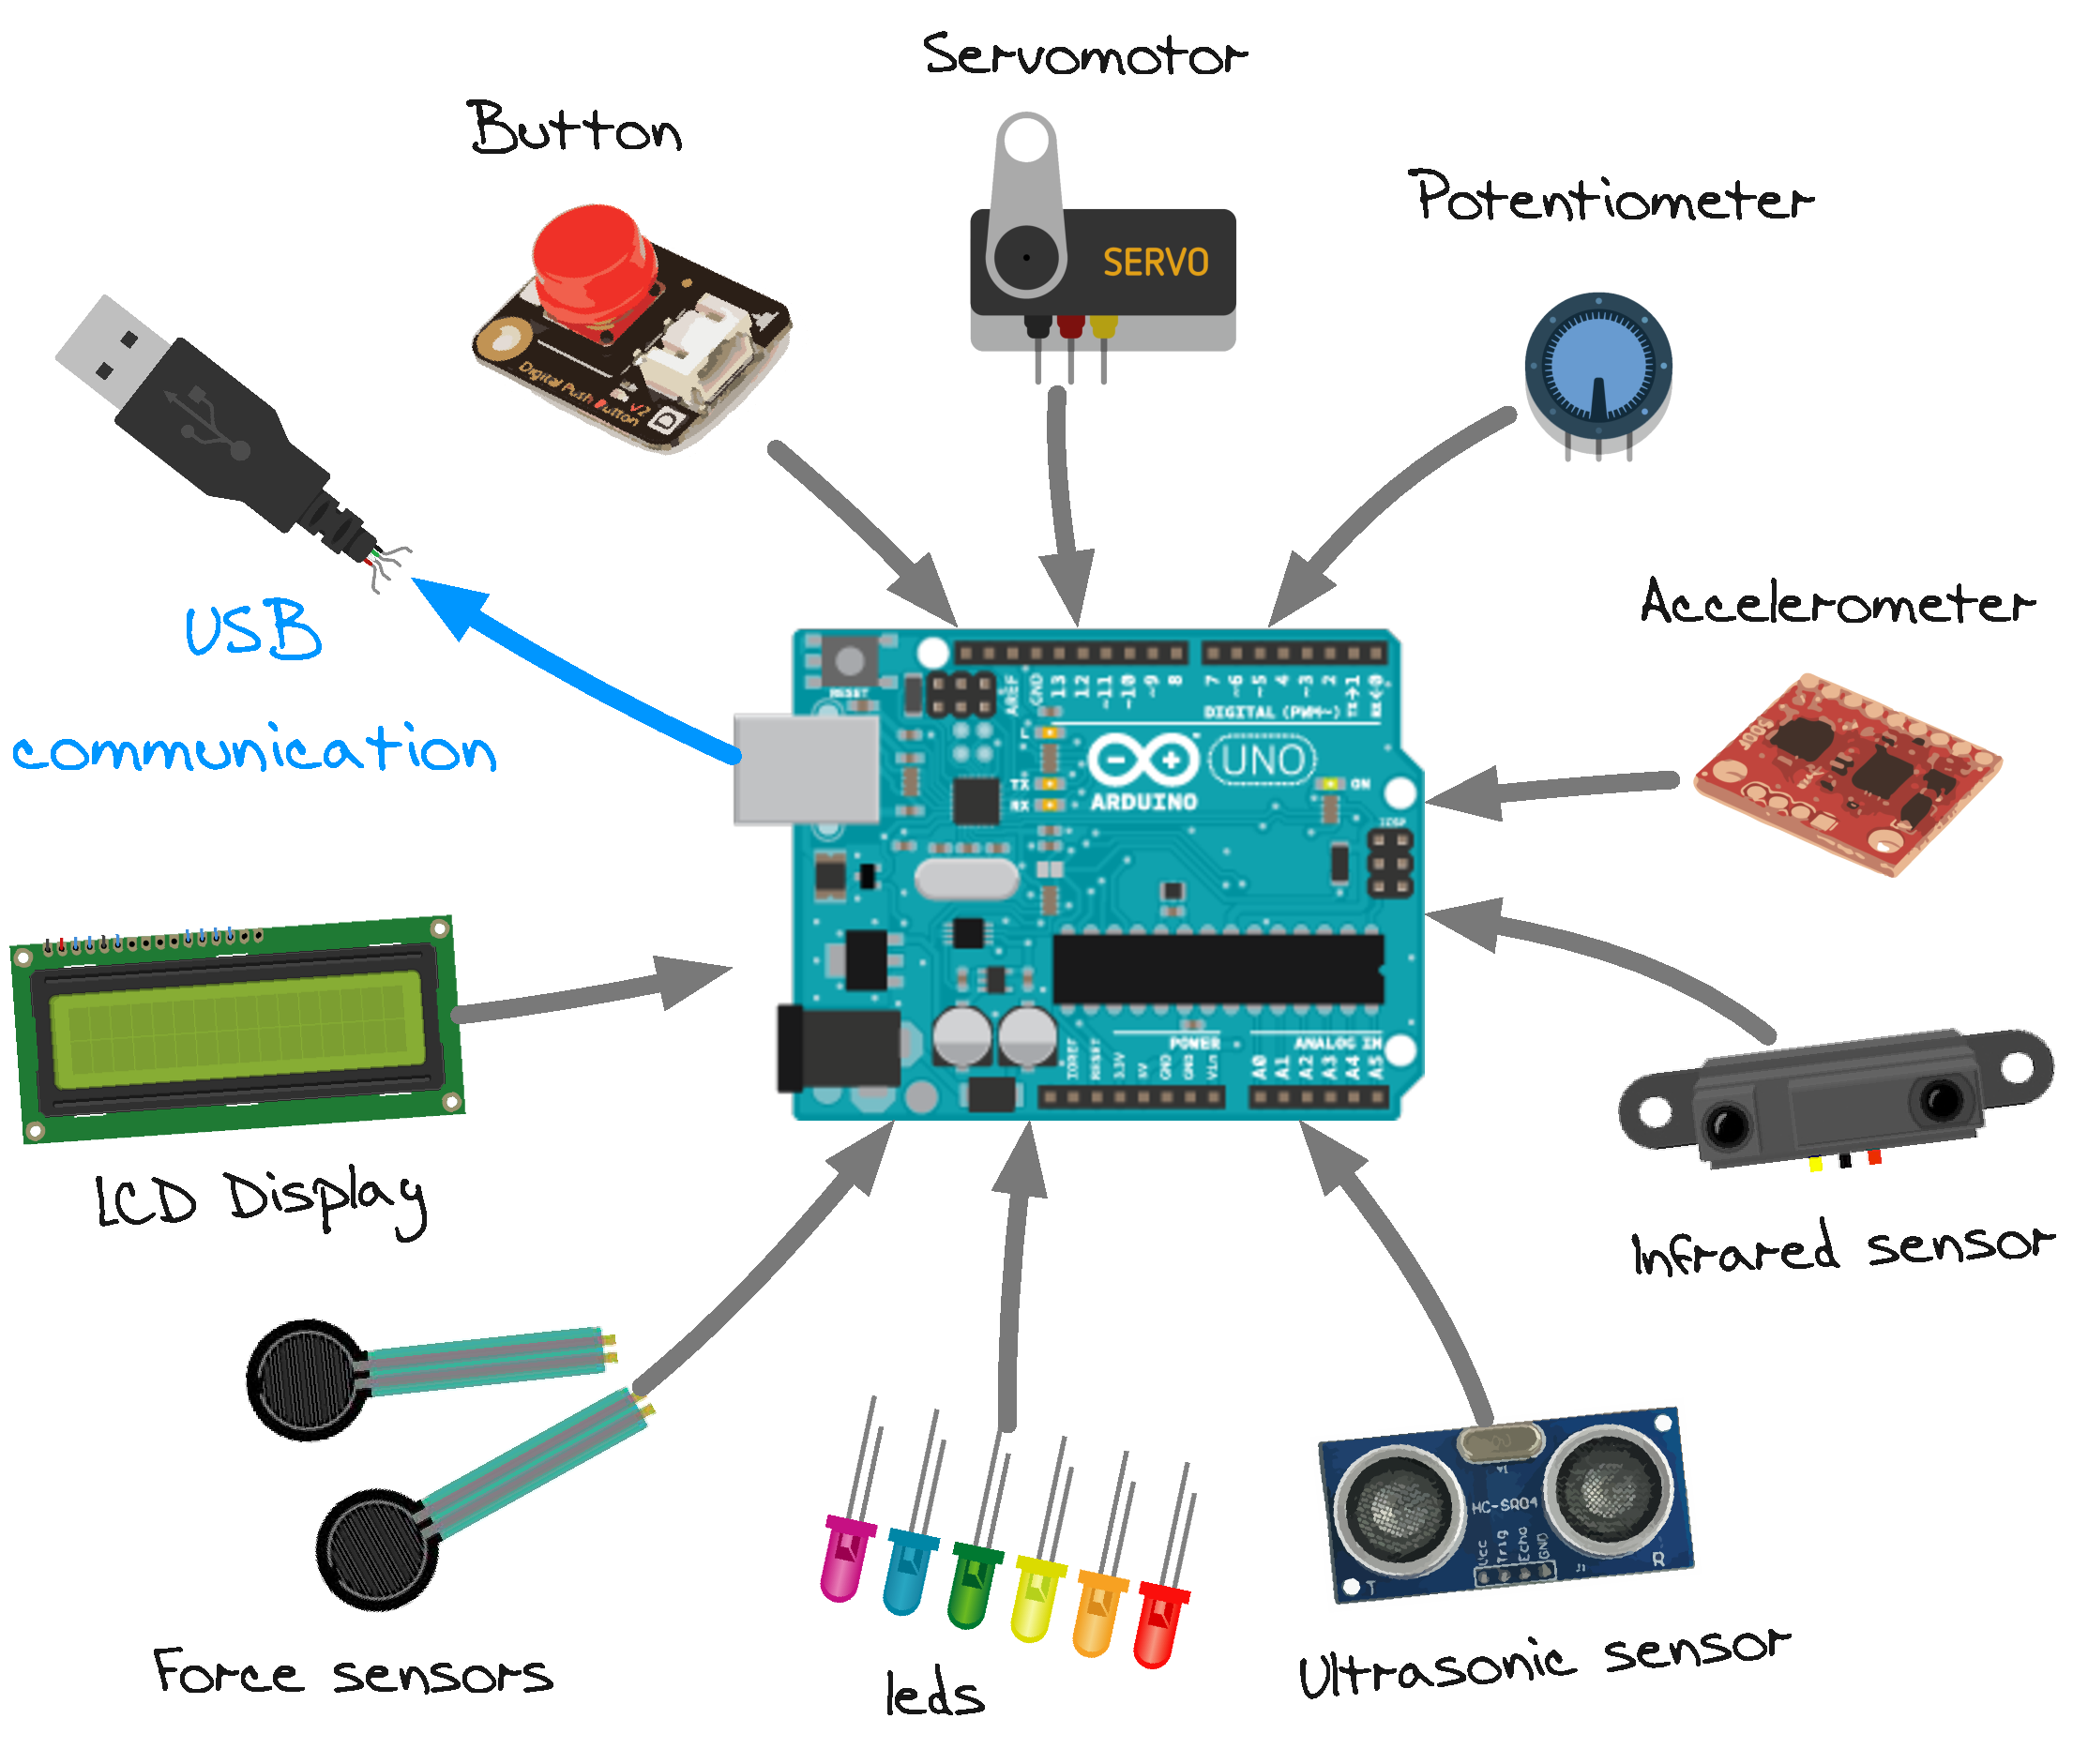
\includegraphics[width=0.9\linewidth]{arduino_electronique.pdf}
    \end{center}
    \caption{The use of Arduino as electronic architecture  allows for sensors to be easily added and/or changed, while keeping the same electronic board. In addition, it permits to add expressive components such as LEDs, LCD or sound systems, allowing users to easily explore human-robot interaction.}
    \label{fig:arduino_modular_electronic}
\end{figure}


The Arduino community is very active and expanding, more and more sensors are designed to be directly plugged onto Arduino boards. Thus, using Arduino adds modularity to robot electronic architecture, allowing the reconfiguration of the sensors space by easily adding new ones (see \figurename~\ref{fig:arduino_modular_electronic}).


\subsection{All-in-one actuators} % (fold)

As we explained briefly in REF, several techniques are available to make robots move from classic and cheap servomotors to the highly powerful and dynamic hydraulic actuators powering the Atlas humanoid robot.
While some actuator technologies such as Series Elastic Actuator (SEA), cable-driven or artificial muscles are really promising to create more robust and efficient robots, they are still work-in-progress solutions and require advanced skills both to assemble and use. These technologies are not yet compatible with the creation of diffusible and reproducible robotic platforms in a multidisciplinary research community.

% \textbf{TODO: Image de system mecanique avec cable ou air }

To permit the diffusion, we need off-the-shelf and stationary solutions, easy to assemble, easy-to-use and available anywhere. Also, to allow the exploration of morphology, actuators have to be modular and allow the tuning of several parameters.

We therefore chose to use Robotis Dynamixel servo-motors\footnote{\url{http://www.robotis.com/xe/dynamixel_en}} for robot actuation (see \figurename~\ref{fig:dynamixel_models}). Dynamixel motors are easily accessible, as they are mass produced and shipped worldwide. Also they are the most commonly used actuators in the robotic field and many robots are powered by them, including Darwin-OP~\parencite{ha2011development}, Myon~\parencite{hild2012myon} , Acroban~\parencite{ly2011bio} or Nimbro~\parencite{schwarznimbro}.

The Dynamixel motors are not simple servomotors, they are all-in-one-modules that contain drivers, encoders and communication buses. They are also quite powerful, robust and rather precise. This is achieved by the combination of Maxon motors, metal gearbox and precise magnetic rotation sensor (resolution: 0.1\textsuperscript{o}). They embed a 32bits micro-controller dedicated to communication (serial port TTL or RS232), the control of the joint (position, speed or torque) and the measurement of internal data such as the real position, speed, load or temperature. They also allow tuning the internal PID or limitation of the maximal torque. This enables rich behaviour, useful both for physical interaction and locomotion.


\begin{figure}[tb]
\centering
    \subfloat[][Robotis Dynamixel AX and MX series]{\label{fig:dynamixel_models}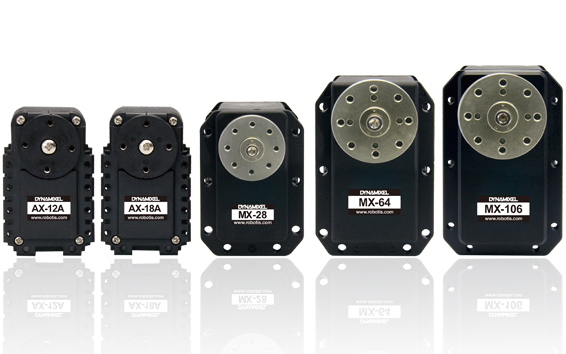
\includegraphics[width=0.48\linewidth]{dynamixel_actuator.jpg}}
    \hfil
    \subfloat[][Power of each Dynamixel model]{\label{fig:dynamixel_powa}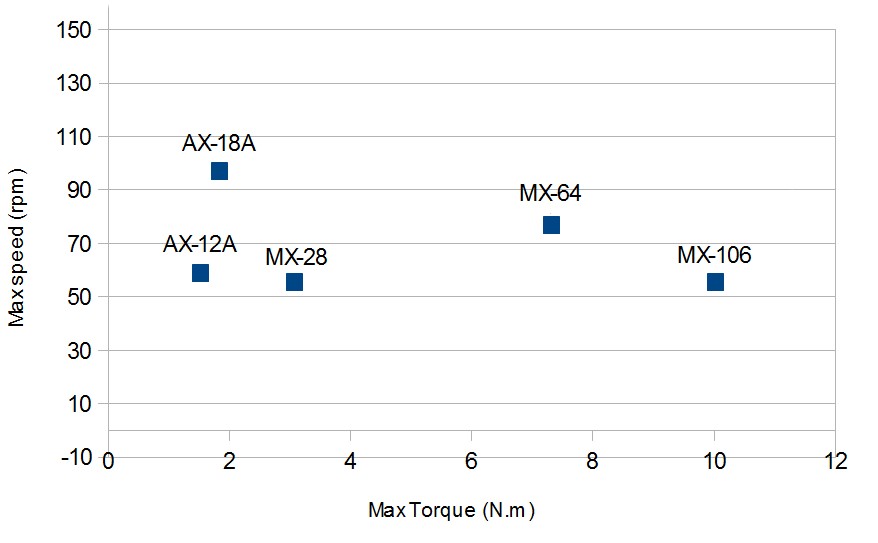
\includegraphics[width=0.48\linewidth]{comparaison-servomoteurs-dynamixel-robotis.png}}\\
    \caption{The Robotis Dynamixel come with different models from low cost ones such as AX-12/18 to the most powerful MX-series with maxon motor and magnetic encoder.}
    \label{fig:dynamixel_serie}
\end{figure}

Different models are available and permit the adjustment of the actuation to the power required by the joint (see \figurename~\ref{fig:dynamixel_powa}). They are different in size and power but their API remains the same and we can easily switch from one to another without changing the code or the electronic integration. Yet, even if the size changes, the foot-print keeps the same pattern (see \figurename~\ref{fig:dynamixel_dimension}) which make easy-to-configure parametric mechanical parts, it just takes a couple of minute to transform a part designed to be compatible with Dynamixel MX-28 to one compatible with Dynamixel MX-64.


\begin{figure}[tb]
    \begin{center}
        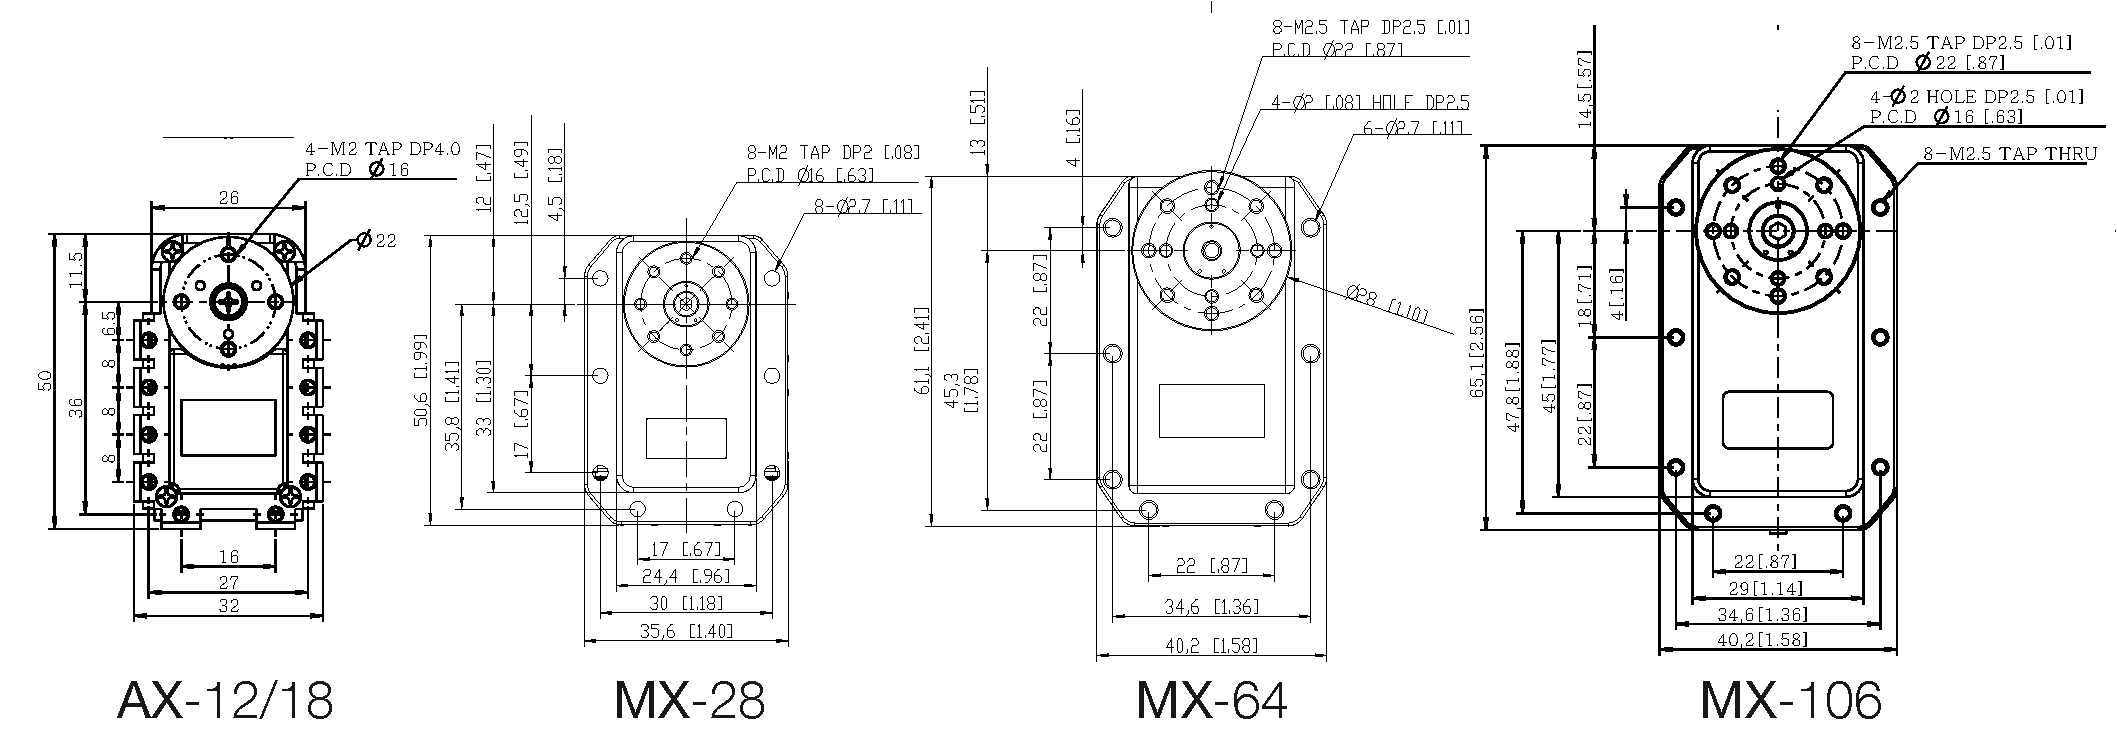
\includegraphics[width=\linewidth]{dynamixel_dimension.pdf}
    \end{center}
    \caption{The footprint of Dynamixel motors keeps the same pattern, only the dimensions are increased following the power of the motor. Thus, switching from one model to another only requires changing the dimension and not the design of a part. With parametric software such as as Solidworks, it takes a couple of minutes to modify a mechanical part to be compatible with another Dynamixel motor.}
    \label{fig:dynamixel_dimension}
\end{figure}


\subsection{Accessible and extensible software} % (fold)

Having variability in software is more classical. Here the choice has been made in favour of ease-of-use and modularity. We design sensory-motor control API adapted to the hardware variability we have. We choose to use Python as the main programming language as it allows fast development, easy deployment on all operating systems and quick scripting by non-necessary expert developers. It also offers a large variety of scientific and machine-learning libraries used in robotics (e.g. Numpy, Scipy, Scikit-learn).
This language is rather slow compared to C or Java, but sensorimotor control is done using serial bus communication and as the serial communication is handled through the standard library we can still achieve rather high performance.

\subsection{Open source distribution} % (fold)

Finally, while the main aspect of such an approach is to allow variability, reuse and modification of the initial design, it is necessary to not only diffuse our work through scientific publications but also to distribute the material needed.
This means anyone outside the Flowers lab should have access to the actual source files and be free to make any changes suitable to their own research. Therefore in addition to the technological choices previously presented, we decided to distribute all our work (both software and hardware) under open source licenses.
This is an essential step toward building new research tools that facilitate both scientific validation and cumulative science in robotics. We will discuss this in detail in the next section.


\section{Allowing cumulative and Open science} % (fold)

As we explained previously, new design approaches and methods should be used to create robots with morphology that can be explored by the user. In addition, by choosing the relevant technologies, we can permit both  the easy exploration of morphological variants, and the transfer and exchange between research laboratories.

To head in this direction, an unfettered access to knowledge and the components associated (articles, data, software, materials, methods) is needed. Also, it is preferable that work can be built upon without asking permission and where the methodology is increasingly based on open collaboration.

A very well adapted tool is the open-source license, which allows the source code, blueprint or design to be used, modified and/or shared under defined terms and conditions. The terms and conditions are defined by several different licenses and the author can choose among them the one that best suits the level of freedom  with which he wants to distribute his work. These licenses are famous and widespread in software development and have started to be used for hardware over the last  few years (see chapter REF).

Nevertheless, in Science the preferred distribution channel is still primarily based on paper publishing and only a few researchers distribute their work under open source license. It is surprising as the use of open source collaboration seems very desirable for scientific research, especially in the robotic field:

\begin{description}
    \item[Scientific validation]: Similarly to publishing detailed mathematical proofs, sharing materials associated with a robotics experiment permits serious peer-reviewing, fundamental for the scientific validation of our field.
    Indeed, robotics experimentation involves a large amount of material (both software and hardware), reviewers should be able to evaluate if the material and experimental setup are coherent with the results submitted.

    \item[Open Science:] We often use only one part of the data collected in an experiment. The open distribution of all material allows the reuse of experiments by other researchers, who can use the same data to extract alternatives or extend the initial results.
    It also permits access to all details and especially to the constant parameter tuning, very sensible for a number of algorithms.

    \item[Cumulative Science] Most of the time, only a scientific paper is published. If this paper presents an algorithm or a mechanism, interested researchers have to reverse-engineer the entire development process. Either the researcher will have to waste time o doing this or he will not use this work at all.
    Finally, it permits mutual aid between researchers, which helps to debug or improve performance.

\end{description}


Yet placing all material we have on the web with an open source license is not enough to achieve the goals previously mentioned. As a paper has to be well written in a clear, precise and concise manner, associated material has to be understood and directly usable.
Therefore, there is a considerable amount of extra work required to permit fluent and effective open collaboration:
\begin{itemize}
    \item Since the work is intended to be reused by external and hopefully numerous of people, the sources have to be clean, robust and well-documented. In addition, some how-to tutorials are very welcome.
    \item A versioning tool should be set up to track changes and efficiently manage a collaborative workflow.
    \item Online community tools should be set up to host discussions between researchers.
\end{itemize}

This work can increase the overall development time by a factor of 3 but participates both in building cumulative science in the research community and increasing the actual impact of our work.

In the Poppy project we decided to distribute all the hardware under "copyleft" licenses, which let users freely use the sources as they want on the condition that they share the derivative work with the same license.
The open source distribution and community management will be discussed with more details in the chapter REF.


\section{Conclusion} % (fold)

In this thesis, we aim to enable both the free exploration of morphological variants on real robotic platforms and their diffusion in the research community. To do so, we suggest exploring an alternative design based on 3D printing for mechanical parts, Arduino electronic architecture for sensors, Robotis Dynamixel motor for actuation and Python API for control.

This design process permits the creation of low-cost and highly hackable experimental robotic platforms thanks to a fully modular and open source approach.

The tools used form part of the makers revolution and the emergence of the new rapid prototyping tools, sometimes called the novel industrial revolution~\parencite{anderson2012makers}. Therefore we can rely on the hundreds of Fablabs around the world as a lever arm to increase the dissemination and reproducibility of robotic platforms designed with such methods.

Yet the chosen approach raised some limitations. Indeed, since we want to keep our work reproducible, we have to reduce the complexity of the assembly as well as the use of our robotic platforms. This means we need to spend more time developing and testing our design to make it as easy to use as possible. Also we are limited in the components we can use, they have to be easily accessible i.e. easily available and in large quantities in online stores.

Also, for the open source distribution, essential in creating a research community platform, a lot of effort is required to create an efficient and pleasant workflow.

In the next chapter, we will explain how we applied the methodology presented to the design of a whole new humanoid robot called Poppy. Then, in the chapter REF, we will discuss the open source distribution and how we manage the community.






% !TEX root = ../../thesis.tex

\cleartoleftpage
\includepdf{../media/chapter_illustration/papaver_rhoeas}



\chapter{The Poppy development} % (fold)


\section{Introduction} % (fold)

Research in humanoid robotics has been thriving in the recent years~\cite{hirai1998development} \cite{kaneko2008humanoid}, both due to theirs predicted relevance for personal and assistive robotics~\cite{tapus2007socially} \cite{oztop2005human}, and because of the scientific challenges raised by robotics with regards to cognition~\cite{asada2001cognitive}, natural communication~\cite{stiefelhagen2004natural} \cite{breazeal2002robots}, biped locomotion~\cite{yamaguchi1999development} \cite{chestnutt2005footstep} \cite{collins2005bipedal} and full-body physical interaction with the environment~\cite{ude2004programming}.

But like the LHC is an experimental platform allowing to explore quantum mechanics and the origin of our universe,  humanoid can act as simplified and controllable human simulator. Thus humanoid robots can be amazing tools to study human-being and eventually contribute in a better understanding of Human's behaviors and abilities~\cite{atkeson2000using} \cite{cheng2007cb} \cite{brooks1986achieving}.

A famous example of such humanoid uses was the Cog project~\cite{brooks1999cog} at the Humanoid Robotics Group of the Massachusetts Institute of Technology. This research project has two goals: an engineering goal of building a prototype general purpose flexible and dextrous autonomous robot and a scientific goal of understanding human cognition~\cite{brooks1994building}. In particular, this project concentrated on embodiment and interaction intelligence with four aspects of a novel methodology: developmental structure, physical embodiment, integration of multiple sensory and motor systems, and social interaction. For this purpose they build several robotic platform such a humanoid~\cite{brooks1999cog} (see \figurename~\ref{fig:brooks_and_cog}), and a very expressive multi-articulated head named Kismet~\cite{breazeal2003emotion} (see \figurename~\ref{fig:breazeal_kismet}).

% This project ended in 2003 and has bring great scientific contributions such as ... REF


\begin{figure}[t]
\centering
    \subfloat[][Rodney Brooks and the Cog humanoid]{\label{fig:brooks_and_cog}\includegraphics[height=5cm]{brooks_and_cog.jpg}}
    \hfil
    \subfloat[][Cynthia Breazeal with Kismet]{\label{fig:breazeal_kismet}\includegraphics[height=5cm]{breazeal_kismet.jpg}}
    \caption{The Cog project was about the use of computer and robotic technology to better understand and emulate human intelligence.}
    \label{fig:cog_project}
\end{figure}



The context of this PhD thesis is grounded on the same scientific motivations as the work of R.Brooks, R.Pfeifer, T.McGeer and initiative such as the Cog project i.e. exploring the role of morphology, cognition and embodiment intelligence in several aspects using real experimental robotic platforms.

The scientific approach of the Cog robots is oriented toward the exploration of embodiment in several aspects, from the low level mechatronics to head design for social interactions, but they were built 15 years ago and using classic manufacturing technique (see \figurename~\ref{fig:cog_project}) that made them expansive, complicated to be modified and especially difficult to diffuse in other laboratories.
We are now in 2014, the makers revolution is in progress~\cite{anderson} and novel technologies allows to rethink the way we design robotic platforms, especially humanoid.

In the previous chapter we presented a methodology to design robotic platform allowing both a free exploration of morphological variations and the diffusion in the research community. This method uses 3D printing to produce mechanical part, Arduino architecture for the electronic system and python-based API for the control.

We think such design methodology can contribute in building better experimental robots while it allows to make the modification of a robot morphology both easy and low cost, and by the use of open source diffusion, it permits the transfer and the reuse of scientific work in other laboratories.
Within this context we built a whole new humanoid robot called PoppyTM (see Fig.~\ref{fig:poppy_with_me}).

\begin{figure}[tb]
    \begin{center}
        \includegraphics[width=0.7\linewidth]{lapeyre_and_poppy.jpg}
    \end{center}
    \caption{Poppy}
    \label{fig:poppy_with_me}
\end{figure}

This humanoid robot is designed to easily and quickly conduct scientific experiments on sensorimotor learning, exploring morphological properties, and human-robot interaction. As an experimental robotic platform, Poppy is designed to be \textbf{affordable}, \textbf{lightweight}, \textbf{robust and safe}, \textbf{easy to use}, \textbf{highly-hackable} and \textbf{fast and easy to duplicate or modify} with the goal to be easily reproducible and used by other lab thanks to an open source distribution (hardware and software).

In this chapter,  we will describe our motivation, the design guidelines we have followed and the conception of Poppy.


\section{Creating a novel humanoid robot} % (fold)

\subsection{Motivations} % (fold)

In 2012, when we started this work, none of the existing humanoid platforms were suitable for exploring the role of morphology. There were two kind of platform. On one hand the commercial robots, rather easy to use and accessible but with a static and frozen morphology. On the other hand, prototype robots produced in labs to adresse specific experimentations, studying interesting morphologies but complicated to use and impossible to reproduce outside the lab.

In our lab, we had both kind of robot. We used Nao (see \figurename~\ref{fig:nao_platform}) to study human robot interaction (REF PIERRE cadeau). It was really convenient to be use by researchers those are not comfortable with get their hands dirty and do not really care about hardware issue while their are addressing more high-level research challenges. Yet such platform is limited as it is not possible to modify it if the robot is not adapted to our experiment. For example back at this time the Nao camera was not efficient, we have difficultly achieved 5 frames/seconds.
We had the necessary skills to hack Nao and change the camera but its hardware is not designed to be changed. Improving the vision performance could only be possible by the addition of an external camera on the Nao head which would ruin the user experience.

\begin{figure}[]
\centering
    \subfloat[][Nao]{\label{fig:nao_platform}\includegraphics[height=5cm]{nao_face.png}}
    \hfil
    \subfloat[][Darwin-Op]{\label{fig:darwin_platform}\includegraphics[height=5cm]{darwin_op_face.jpg}}
    \hfil
    \subfloat[][Acroban]{\label{fig:acroban_platform}\includegraphics[height=5cm]{acroban_wout_background.jpg}}
    \caption{None of the existing platform in 2012 was suitable to explore the role of morphology. Nao was impossible to modify. Darwin Op and Acroban used aluminium part really difficult and expensive to produce.}
    \label{fig:2012_Humanoids}
\end{figure}

We also used Acroban (see \figurename~\ref{fig:acroban_platform}) designed in our team by Olivier Ly~\cite{Ly2010}. It is a handcrafted humanoid platform created to explore morphological properties, especially compliance toward the achievement of dynamic locomotion and playful physical human robot interaction.
While it actually allows modification of its is morphology, its manufacture based on aluminum mechanical parts, Robotis Dynamixel motors, scotch, and rubber bands cobbled together therefore requires lot of effort to be changed. Especially the manufacture of aluminum parts require specific skills and tools.
Also its use was quite complicated and while several researchers could have been interested by Acroban to study human robot interaction and social acceptance, it was not possible to use it without getting our hands dirty.
Finally, the material and manufacture process make platform non-stationary, even if a lab manage to reproduce it, there is a high probability that the physical properties will not be the same. Therefore, the diffusion and the reproducibility of results are limited.


A last alternative would be the use of Darwin Op robot (see \figurename~\ref{fig:darwin_platform}) which is both open source and reproducible, yet as Acroban its hardware based on manufactured metal parts make its morphology difficult and expensive to be modified. Moreover to our knowledge, Darwin morphology has never be changed by the research community.

Thus one of the main goals was to achieve the design of a humanoid robot which can merge the advantages of both kind of robot, i.e. simple, accessible, reproducible and allowing to easily change and hack its morphology.

\subsection{A robot experiments-proof} % (fold)

Most researchers can attest of the difficulty and frustration raised by conducting robotic experimentation in the real world. We are daily challenged by bugs, technical issues, unpredicted events and side effects. While a bug in a software can be fixed, an error with a hardware platform can cause damages and postpone the results of an experiment by several weeks.

Therefore many robotic researchers avoid technical issues link with the real world experimentation by using simple model and physical simulation. But the real world is extremely more complex and rich than the virtual one.
Some high-level behavior experiments are conducted in simulator based on the hypothesis that the real world constraints are not relevant, yet it is really sure ?
Indeed, while the real world constitute a lot of constraints, it is also rich of complex physical effects (gravity, friction, inertia) which has to be took in and can be very useful if interacting with the agent.

As we saw in the related work (chapter~\ref{REF}), the emergence of complex behavior can appear thanks to the interaction between the real world and simple robotic system. We cannot program behavior while the behavior is the interaction resultant between the program and the real world. Thus we cannot design behavior without the ecological niche of the robot~\cite{Steels1991emergence}.

While using simulator can be helpful as a first step to design robot, it appears incomplete to show results on the role of morphology without real world experimentations.
Therefore, when ones want to study the role of morphology on the robot behavior, being able to explore it in the real world is of paramount importance.

Along our work on building cognitive and developmental learning algorithms, we had experienced these issues, especially while building and using Acroban~\cite{Ly2010} and during the Ergo robot experience (see section~\ref{REF}).

Therefore Poppy has been designed based on the experience background we have building and using robots acting in the real world.

\begin{description}
    \item[Robustness and Safety:] Heavy and long real-world experimentations imply a robot should be robust and safe. It should be able to sustain experiments and fall down without easily breaking. At the same time, one should ensure that physical interaction with the robot is safe for humans.
    \item [Precision, stationarity:]Experiments should be repeatable, implying that the robot properties should be stationary.
    \item [Breakable, repairable:] Breaking should not be costly and the robot should be easily repairable.
    \item [Transportable:]To allow for experiments in natural environments, possibly involving interaction with non-technical humans, the robot should be transportable outside the laboratory.
    \item [Easy and fast to duplicate:]Such a reuse of the robotic platform requires that it is easy and fast to duplicate.
    \item [Affordable:]
\end{description}


\subsection{Design Guidelines} % (fold)

\begin{description}

    \item[Modular morphology:] The whole structure must be easy to reconfigure both for repairing or hacking purpose. This mean the process to replace a Poppy's parts must be simple, low-cost and not require time or special tooling.

    \item[Less is more: keep it simple:] The fact we want to design an easily reproducible robot means we are limited in our design choices. In most case, finding a simple solution avoid the use of an easy solution: we should minimize the number of part and suppliers, be careful of the availability of our parts in each country, take in account the cost and the assembly complexity. All these constraints make the design of the robot way more complex than a unique prototype robot. It also raises some limitation to the main Poppy version while some interesting or efficient solution cannot be kept due to their complexity.

    \item[A lightweight structure and under-actuated:] Many humanoid robots use powerful motors often associated with highly accurate sensors. This has a cost, both in terms of weight and computation resources. Moreover, to ensure the accuracy of the sensory-motor space it is necessary to design very rigid mechanical parts. The whole structure obtained is powerful but very heavy and due to inertia not very agile. This kind of robots can intensively repeat precise and complex movements, but are somewhat uncomfortable when it comes to walking on uneven ground. All mechanical parts were designed to optimize their weight and make the platform Poppy as light as possible. The obtained mass reduction allows the use of less powerful motors which are therefore lighter. We can thus have a lightweight robot, strong and powerful enough to perform tasks such as walking and physical interaction.

    \item[Bio-inspired morphology:] Human being is a great example of biped locomotion ability. Strictly mimicking the human morphology is certainly not a good idea as the element composing a robot are not comparable. However, studying the functional interest of certain human bio-mechanic properties can reveal interesting insight to explore novel humanoid design.
    \item[Ecological balance principle:] The ecological balance principle, introduce by Rolf Pfeifer, states that there is a balance or task distribution between morphology, materials, control, and interaction with the environment. Following this principle, we try to keep a balance between the different part of the robot.

    \item[Whole body compliance:] Important aspects of adaptation to physical obstacles or HRI require humanoid robots to be full-body compliant. This includes both the ability to absorb external shocks due to the passive compliance of the mechanical structure (bendable materials and springs), but also the ability to actively and dynamically control the compliance of motors, which may be either controlled in position with compliance, or directly in torque (thanks to the use of adequate recent servomotor technologies).

    \item[Take care of the aesthetic:] In the scientific community, design and aesthetic are often left aside as a superficial feature. But when an object has to interact with human, the design and aesthetic represent a main communication channels. The interaction with our senses change the way we understand the purpose of a object. As any communication tool, the message we convey can be noised or enforced by the form. Thus the robot appearance must fit the robot abilities and try to give insights to the user about what it can or cannot do.
    Both at a macro or micro scale, the Poppy aesthetic is thought to show some conceptual aspects of its design, such as the lightness, the modularity or the fact it is not powerful.

\end{description}




% \input{content/chapter/temp2.tex}
% !TEX root = ../../thesis.tex

\cleartoleftpage
\includepdf{../media/chapter_illustration/pypot}
\chapter{Pypot: An open source modular python library for robot control} % (fold)

\section{Introduction} % (fold)

Poppy was designed to be a research platform for freely exploring morphological variations. Although Poppy meets "hardware" needs, control of the platform is also crucial. Whereas more conventional robots have a fixed mechanical and sensorimotor morphology, having a platform that can be fully modified changes the low-level control architecture issues.
We decided to develop a new robotic control library. Called pypot (see \figurename~\ref{fig:pypot_logo}), this library mostly developed by Pierre Rouanet, is adapted to the challenges of morphological exploration and experimentation. Moreover, development begun early in the design of Poppy, and shares the same guidelines and objectives i.e. being robust, modular, versatile and easy to use.


\begin{NFfigure}
    \centering
        \includegraphics[height=5cm]{PyPot_logo_black_transparentbg.png}
    \caption{The logo of the pypot library.}
    \label{fig:pypot_logo}
\end{NFfigure}

To reach these goals, pypot is a library written in Python and developed to make it easy and fast to control custom and modular robots. In particular, pypot has been designed with a simple and easy to use API, a fully modular and customizable architecture, and key-features adapted to robot experimentation issues.

It also shares the open collaboration philosophy and is therefore distributed under an open source GPLv3 license. All sources are available on the associated GitHub repository: \url{https://github.com/poppy-project/pypot}.

Even if pypot has been developed within the context of the Poppy project, in the following sections, most of the code examples will involve an ergo-robot (see \figurename~\ref{fig:ergo-robot}) rather than Poppy to emphasize that pypot is a control library for any modular robot.


\begin{figure}[tb]
\centering
    \subfloat[][]{\label{fig:cpu-load}\includegraphics[height=5cm]{ergo-robot-stem.jpg}}
    \hfil
    \subfloat[][]{\label{fig:pypy-opti}\includegraphics[height=5cm]{ergo-robot.jpg}}
    \caption{Ergo-robot are a 6 DoF serial robots with a stem shape those were developed in the Flowers Lab. In particular, they were involved for the Fondation Cartier exhibition (see chapter~\ref{cha:art})}
    \label{fig:ergo-robot}
\end{figure}


\section{Control of custom robots made simple with pypot} % (fold)

One main preoccupation during the development of pypot was the achievement of a very easy-to-use library for the end user. For this purpose, pypot has been entirely written in Python to allow for fast development, easy deployment (cross-platform) and quick scripting by expert developers that are not necessarily expert developers. In particular, API is simple and permits to write complex behaviours with just a few lines of code.

This is made possible with a layered architecture based on:

\begin{itemize}
    \item Fast and robust low-level API that directly encapsulates the communication protocol for setting and accessing hardware data.
    \item A controller that automatically ensures the update of sensorimotor data (get/set) at a predefined frequency. This method encapsulates the low-level API to prevent the writing of repetitive requests and optimize latency.
    \item Finally, a robot layer can generate automatically a whole robot API giving access to the whole sensorimotor space with just a few lines of code.
\end{itemize}

While low-level layers allow for modularity and customization, the high-level abstracts all the complexity into simple end user API. We will describe more in detail how this architecture works in the next sections.

% Also, it benefits from the Python community with numpy/scipy and machine learning libraries such as scikit-learn.

\subsection{The Dynamixel controller} % (fold)
\label{sub:dynamixel-controller}

Pypot handles the low-level communication with Dynamixel motors from Robotis. Using a USB communication device such as USB2Dynamixel or USB2AX, it opens serial communication with Robotis motors (MX, RX, AX) using communication protocols TTL or RS485. More specifically, it allows easy access (both reading and writing) to the different registers of any Dynamixel motors\footnote{The whole list of registers can directly be found on the Robotis website: \url{http://support.robotis.com/en/product/dynamixel/mx_series/mx-28.htm\#Control_Table}}. Those registers include values such as position, speed or torque.


While the Dynamixel Low-level IO provides access to all functionalities of the Dynamixel motors, it forces us to have synchronous calls, which can take a non-negligible amount of time. In particular, most programs will need to have a really fast read/write synchronization loop, where we typically read all motor positions, speeds, loads and set new values, while we would like to have higher level code that also computes those new values.

On top of the low-level, a Dynamixel controller can be added which defines synchronization loops that will read/write\footnote{Whenever one of the values is accessed, it is actually the most recent versions that have been read at the frequency of the loop.} the registers of Dynamixel motors at a predefined frequency automatically run in the background. Thus there is no need to wait for the answer of a read command to access data (this can take some time) so that algorithms with heavy computation do not encounter a bottleneck when values from motors must be known. The attributes of those "software" motors are automatically synchronized with the real "hardware" motors.

The controller is actually a module (see section~\ref{sub:io-controllers}) and can be changed according to the user’s needs. Yet by default pypot has a base controller, which already defines synchronization loops, more exactly it:

\begin{itemize}
    \item reads the present position, speed, load at 50Hz,
    \item writes the goal position, moving speed and torque limit at 50Hz,
    \item writes the PID or compliance margin/slope (depending on the type of motor) at 10Hz,
    \item reads the present temperature and voltage at 1Hz.
\end{itemize}

This controller embeds very useful synchronization loops, which should be enough for most users.



\subsection{Robot abstraction} % (fold)you
\label{sec:pypot-robot-abstraction}
The robot abstraction allows, from a configuration, to automatically generate both all low-level controllers and high-level accessors needed to control a whole robot. More precisely, through the use of the class Robot it is possible to:

\begin{itemize}
    \item automatically initialize all connections (making the use of multiple USB2 serial connections transparent),
    \item define offset and direct attributes for motors,
    \item automatically define accessors for motors and their most frequently used registers (such as \emph{goal\_position, present\_speed, present\_load, PID, compliant}),
    \item define a read/write synchronization loop that will run in background.
\end{itemize}

The configuration, described as a Python dictionary\footnote{The configuration can be written in the Python script or can be loaded from any file that can be loaded as a dictionary (e.g. a JSON file).}, contains several important features that help build both the robot and the software to manage the robot. The important fields are listed below:

\begin{itemize}
    \item controllers - This key holds the information pertaining to a controller and all the items connected to its bus.
    \item motors - This is a description of all the custom setup values for each motor. Meta information, such as the motor access name or orientation, is also included here. It is also there that we can set the angle limits of the motor.
    \item motorgroups - This is used to define the alias of a group of motors (e.g. \emph{left\_leg}).
\end{itemize}

To give a complete overview of what a config can look like, the \codename~\ref{code:robot_config_file} is an example of the config dictionary of a simple 6-DoF ergo-robot\footnote{Since pypot 1.7, it is possible set the port to 'auto' in the dictionary. When loading the configuration, Pypot will automatically try to find the port with the corresponding attached motor ids.}.


\lstinputlisting[
    language = XML,
    caption = {},
    label = {code:robot_config_file},
    float = p]
    {code/robot_configuration.json}


The robot abstraction encapsulates multiple Dynamixel controllers to read/write all the registers of a robot at a predefined frequency. The user only has to specify the configuration dictionary of his robot using the \emph{from\_config()} function. The robot configuration can also be loaded/saved as a JSON format.

Here is an example of how to create a robot:
\begin{lstlisting}[language = Python]
import pypot.robot

# Load the configuration file
my_robot = pypot.robot.from_config('ergo_robot.json')

# Launch robot sensorimotor synchronization
my_robot = start_sync()
\end{lstlisting}


Then making the robot move is only one line of code:
\begin{lstlisting}[language = Python]
my_robot.base_tilt_lower.goal_position = 120
\end{lstlisting}

In this example, the motor \emph{base\_tilt\_lower} will not reach the 120 degree position, but actually 90 degree because its config file (\codename~\ref{code:robot_config_file}) set the angle limit to \emph{[-90, 90]}.

Therefore the user can set up their robot with just few lines of code and then use it safely just scripting the behaviour they want to achieve.


\subsection{Move recording} % (fold)
\label{sub:move_recording}

Pypot involves a really convenient, yet simple, feature for recording movementss. Indeed, when a robot's motor is compliant (Dynamixel property), a user can demonstrate a desired gesture by physically moving the motor position. Those Moves are simply defined as a sequence of positions.

The move module can be used to:

\begin{itemize}
    \item record moves,
    \item play moves,
    \item save/load them on the disk.
\end{itemize}

Given the same ergo-robot configuration, the recording of a gesture at a 50Hz framerate moving on all motors for 5 seconds can be simply done using the following code:

\begin{lstlisting}[language = Python]
import time
import pypot.robot

from pypot.primitive.move import MoveRecorder, Move, MovePlayer

ergo = pypot.robot.from_config(...)
ergo.start_sync()

move_recorder = MoveRecorder(ergo, 50, ergo.motors)

ergo.compliant = True

move_recorder.start()
time.sleep(5)
move_recorder.stop()
\end{lstlisting}

This move can then be saved on disk:
\begin{lstlisting}[language = Python]
with open('my_nice_move.move', 'w') as f:
    move_recorder.move.save(f)
\end{lstlisting}

And loaded and replayed:
\begin{lstlisting}[language = Python]
with open('my_nice_move.move') as f:
    m = Move.load(f)

ergo.compliant = False

move_player = MovePlayer(ergo, m)
move_player.start()
\end{lstlisting}

This feature seems very simple and anecdotal but is actually one of the most useful pypot features for non-expert users. Indeed it allows to physically "program" the robot and is very intuitive for artists. We will show a demonstration of such a use with Poppy in the chapter~\ref{cha:art}.

% subsection move_recording (end)


\section{Modular environment} % (fold)

Figure \figurename~\ref{fig:pypot-modular-architecture} shows the pypot 2.x architecture and especially its modularity. Indeed pypot has a modular architecture both for the low-level communication with the robot and for the high-level behaviour control. This modularity allows pypot to be adapted to:

\begin{itemize}
    \item morphological exploration because it permits to switch between several low-level controllers with respect to the hardware properties of the robot (i.e. sensors, motors),
    \item scientific experimentation because its high-level modularity allows to easily run behaviour and extend the control to other libraries.
\end{itemize}

This modularity is expressed through the I/O controllers and the primitive paradigms, which will be, discussed in detail in the next sections:


\begin{figure}[p]
    \begin{center}
        \includegraphics[width=\linewidth]{pypot.pdf}
    \end{center}
    \caption{}
    \label{fig:pypot-modular-architecture}
\end{figure}


\subsection{I/O controllers} % (fold)
\label{sub:io-controllers}

The low-level Dynamixel controller presented previously (see section~\ref{sub:dynamixel-controller}) is actually an instance of an I/O controller. The I/O controllers are the interface between real world data acquisition and the pypot core. They constitute the low-level modular part of pypot and allow for anyone to create a custom controller adapted to particular robot properties.

A brilliant example of this modular I/O controller architecture is the control of the robot either in the simulator or the real world just by switching between I/O controllers:

\subsubsection{Switching between the simulator and the real world} % (fold)

As it is often easier to work in simulation rather than with the real robot, Pypot has been linked with the V-REP simulator\footnote{\url{http://www.coppeliarobotics.com/features.html}}. It is described as the “Swiss army knife among robot simulators” and is indeed a very powerful tool to quickly (re)create robotics setup. Moreover, we chose to integrate this particular simulator first because it shares distinctive features with the Poppy project, i.e. being cross-platform, easy-to-use, extensible and open source\footnote{Actually V-REP has a double license Commercial/GPL so either one pays and can keep his customizations or has to release all modification under GPL.}

\begin{figure}[tb]
    \begin{center}
        \includegraphics[width=\linewidth]{pypot_vrep.jpg}
    \end{center}
    \caption{}
    \label{fig:pypot-vrep}
\end{figure}


The connection with V-REP was created using the I/O controllers presented previously and the V-REP’s remote API.
Thanks to the low-level modularity of pypot, it permits to seamlessly switch from your real robot to the simulated one because it only requires switching the low-level I/O controller from the Dynamixel (\emph{DxlController} class) one to the V-REP one (\emph{VrepController} class).

The switch between the simulation and the real robot is possible with a single line of code, and in most case, only requires changing the way the robot is instantiated see \codename~\ref{code:vrep_pypot_switch}.

\lstinputlisting[
    language = Python,
    caption = {},
    label = {code:vrep_pypot_switch},
    float = ht]
    {code/vrep_pypot_switch.py}

In addition, it provides some extended features relative to the needs we have in a robot simulator, among them:
load a scene, start/stop/restart a simulation, pause/resume the simulation, get an object position/orientation.
Yet not all Dynamixel registers have their V-REP equivalent. For the moment, only the control of the position is used but it will be extended in the future. Also more advanced features can be easily added thanks to the controller abstraction.


\subsubsection{Custom I/O controllers} % (fold)

The I/O controller is actually defined by two classes:

\begin{itemize}
    \item the IO class defining how to communicate with an object (i.e. motor or sensor) and obtain its data,
    \item the controller class defining all object properties the robot can access and control.
\end{itemize}

It is therefore possible to extend the number of controllers to any connected object. For example, it could be used to change the type of motors used and replace the Robotis motors with more low-cost ones, or to control a robot with a simulator other than V-REP, and the switch should be as straightforward.


\textbf{TODO put code ?}


\subsubsection{Automatic generation of the robot} % (fold)
In the same way that the pypot robot class can automatically create a robot based on Dynamixel motors and generate an easy-to-use API, it can handle the variability of the I/O controllers. Indeed the desired I/O controllers can be indicated during the robot configuration then the robot will be generated in accordance with the specified controllers. The v-rep simulator is an example of such use (\codename~\ref{code:vrep_pypot_switch}).

Thus the pypot robot can handle multiple controllers both for motor control and for the sensors acquisition (e.g. IMU, tactile, camera).


\subsection{Primitive paradigms} % (fold)
\label{sub:primitive-paradigms}

The high-level modularity of pypot is expressed by the primitive paradigms. We call a Primitive any simple or complex behaviour applied to a Robot. A primitive can access all sensors and effectors in the robot. A primitive is supposed to be independent\footnote{The independence of primitives is really important when one creates complex behaviours - such as balance - where many primitives are needed. Adding another primitive - such as walking - should be direct and not force the rewriting of everything. Furthermore, the balance primitive could also be combined with another behaviour - such as shooting a ball - without modifying it.} from other primitives. In particular, a primitive is not aware of the other primitives running on the robot at the same time. We imagine those primitives as elementary blocks that can be combined to create more complex blocks in a hierarchical manner.

To ensure this independence, the primitive is running in a sort of sandbox. More precisely, this means that the primitive does not have direct access to the robot. It can only request commands (e.g. set a new goal position of a motor) to a Primitive Manager, which transmits them to the “real” robot. As multiple primitives can run on the robot at the same time, their request orders are combined by the manager\footnote{The primitives all share the same manager. In further versions, we would like to move from this linear combination of all primitives toward a hierarchical structure and have different layer of managers.}.

The manager uses a filter function to combine all orders sent by primitives. By default, this filter function is a simple mean but you can choose your own specific filter (e.g. add function).

To write a primitive, the user only needs to create a subclass of the Primitive class. It provides basic mechanisms (e.g. connection to the manager, setup of the thread) to allow the direct “plug” of novel primitives to a robot and run it.

Currently there are two kinds of primitives.


\lstinputlisting[
    language = Python,
    caption = {},
    label = {code:primitive},
    float,
    floatplacement = h]
    {code/primitive.py}

\lstinputlisting[
    language = Python,
    caption = {},
    label = {code:loop_primitive},
    float,
    floatplacement = h]
    {code/loop_primitive.py}

The primitive can be start(), stop(), pause() and resume(). Unlike a regular python thread, a primitive can be restarted by calling the start() method again.

When overriding the Primitive, you are responsible for correctly handling those events. For instance, the stop method will only trigger the \emph{should\_stop} event that you should watch in your run loop and break when the event is set. In particular, you should check the should\_stop() and should\_pause() in your run loop. You can also use the wait\_to\_stop() and wait\_to\_resume() to wait until the commands have actually been executed.


\lstinputlisting[
    language = Python,
    caption = {},
    label = {code:start_primitive},
    float,
    floatplacement = h]
    {code/start_primitive.py}

\lstinputlisting[
    language = Python,
    caption = {},
    label = {code:attach_primitive},
    float,
    floatplacement = h]
    {code/attach_primitive.py}

The move feature described in section~\ref{sub:move_recording} is actually based on the pypot primitive paradigm. More precisely, the \emph{MoveRecorder} and \emph{MovePlayer} are defined as a subclass of \emph{LoopPrimitive}.

\subsection{Extensible API} % (fold)

We added the possibility to remotely access and control your robot through the TCP network. This can be useful both to work with client/server architecture (e.g. to separate the low-level control running on an embedded computer and higher-level computation on a more powerful computer) and to allow you to plug your existing code, written in another language, into the pypot’s API.

We defined a protocol that allows all the robot variables and methods (including motors and primitives) to be accessed via a JSON request. The protocol is entirely described in the section Protocol below. Two transport methods have been developed so far:

\subsubsection{HTTP server} % (fold)

The \emph{HTTPServer }is based on the bottle python framework (http://bottlepy.org/). We have developed a sort of REST API based on the protocol described above:

\begin{itemize}
    \item GET /motor/list.json
    \item GET /primitive/list.json
    \item GET /motor/<name>/register.json (or GET /<name>/register.json)
    \item GET /motor/<name>/<register> (or GET /<name>/<register>)
    \item POST /motor/<name>/<register> (or POST /<name>/<register>)
    \item POST /primitive/<prim\_name>/call/<meth\_name> (or GET /<prim\_name>/call/<meth\_name>)
    \item POST /request.json
\end{itemize}


\lstinputlisting[
    language = Python,
    caption = {},
    label = {code:http_server},
    float,
    floatplacement = h]
    {code/http_server.py}


\subsubsection{ZMQ server} % (fold)

The Zmq Server used a Zmq socket to send (resp. receive) JSON request (JSON answer). It is based on the REQ/REP pattern. So you should always alternate sending and receiving. It will probably be switched to PUB/SUB soon.

Zmq has been chosen as it has been bound to most languages\footnote{\url{http://zeromq.org/bindings:_start}} and can thus be used to connect code in other languages to pypot. For instance, we used it to connect RLPark\footnote{RLPark is a Java reinforcement learning library developed by Thomas Degris to experiment with online learning algorithms on robots and benchmarks, see \url{http://rlpark.github.io/}} to pypot.

The Zmq server is faster than the HTTP version and should be preferred when working with high frequency control loops.

\lstinputlisting[
    language = Python,
    caption = {},
    label = {code:zmq_server},
    float,
    floatplacement = h]
    {code/zmq_server.py}


In particular, those for which the extension could be used to create a monitor interface using web technology.



\section{Discussion} % (fold)

\subsection{Why not using ROS instead ?} % (fold)

One famous robotics software is the Robot Operating System\footnote{The Robot Operating System (ROS) is a flexible framework for writing robot software. It is a collection of tools, libraries, and conventions that aim to simplify the task of creating complex and robust robot behaviour across a wide variety of robotic platforms.}. ROS is very widespread in the research community and one could quite rightly question the choice we made in creating a whole new architecture rather than using a well-known and efficient one.

Actually ROS has several aspects that do not fit in with the objectives we have. Indeed, using ROS is not a simple task. The installation is only recommended on one precise Ubuntu distribution\footnote{ROS Hydro only supports Precise, Quantal, and Raring for debian packages \url{http://wiki.ros.org/indigo/Installation}}, and the whole architecture is of course powerful but difficult to set and maintain. Also changing the low-level is complex and requires hacks, sometimes not very elegant ones. Finally, ROS require high computational power, which make it difficult to embed on small computers.

In the Poppy project, we are trying to create a multidisciplinary robotic community, involving as a result, non-robotics experts. Thus, we endeavour to bring down the complexity of using Poppy. To reach this goal, we need a simple user interface/API and a lightweight library, easy to setup whichever system used. Finally, ROS is very modular for high-level but we desire to have modular low-level control.

For all the reasons mentioned above, we considered it to be more simple and effective to create a novel lightweight robot control library rather than adapting ROS to our needs.


\subsection{Limitations} % (fold)

The pypot library is currently rather mature and robust, yet there remain some limitations that are challenging to a variable degree.

\subsubsection{Performances}

Pypot is written in python because it allows fast development and simple API for non-expert users. Also the main goal of pypot is to be an easy-to-use prototyping environment so users can run complete experiments with a custom robot in a couple of minutes to few hours. These choices imply a number of layers and multiple calls of functions, slowing the general execution of the code.

While it is not a problem on modern personal computers, it is more limiting on very light configurations (see \figurename~\ref{fig:pypot-board-comparaison}). For example, running pypot on a Raspberry Pi takes all CPU resources and the sensorimotor acquisition of Poppy at $50Hz$ (i.e. $<20ms$) is not achieved.
The performance could be improved by splitting pypot with the low-level executed on

\begin{figure}[tb]
    \begin{center}
        \includegraphics[width=0.7\linewidth]{board-cmp.pdf}
    \end{center}
    \caption{Time spent to communicate with one motor.}
    \label{fig:pypot-board-comparaison}
\end{figure}

\begin{figure}[tb]
\centering
    \subfloat[][ CPU load during pypot run]{\label{fig:cpu-load}\includegraphics[width=0.5\linewidth]{cpu_load.pdf}}
    \hfil
    \subfloat[][Time spend to synchronize the 25 Poppy's motors]{\label{fig:pypy-opti}\includegraphics[width=0.5\linewidth]{controller.pdf}}
    \caption{}
    \label{fig:pypot-run}
\end{figure}



\subsubsection{The primitive paradigms: The Good, the Bad and the Ugly}
\label{sec:pypot-primitives-problems}

The use of primitives (see section~\ref{sub:primitive-paradigms}) raises some complicated limitations. Indeed it is really convenient to run complex behaviours by splitting them into more simple ones but the interaction between primitives is really complex to manage and can lead to undesired behaviours. Indeed, while multiple primitives can request to change the same value, the final value is the result of the combination (e.g. mean, sum) of several primitives.


It is a case of emergent behaviour\footnote{Finding the rules that can lead to a desired behaviour is more difficult than explaining the real, observable complex behaviour of an agent interacting with its environment. Since the behaviour itself cannot be preprogramed but is always the result of an agent-environment interaction, we must design for emergence rather than directly for a specific behaviour~\parencite{Pfeifer06}.} problem as explained in chapter~\ref{cha:morphology-review}, but at the control software level. It is really interesting because it forces us to design  for emergence as explained by Steels~\parencite{Steels1991emergence}, yet it is still challenging to explain to the end user and in particular to non-expert ones.


\section{Conclusion} % (fold)

As explained in this chapter, Pypot is a modular robot control library, simple to use and extendable to the needs of users. Moreover its very modular low-level permits to easily manage morphological variability while its high-level primitive paradigm permits to quickly run more or less complex behaviour on the robot.

Pypot is open source and distributed under GPLv3 license. All sources are available on the GitHub repository of the project: \url{https://github.com/poppy-project/pypot}. Also the complete documentation can be accessed here: \url{https://poppy-project.github.io/pypot/}.


% subsection _ (end)

% The high-level design allows the use of primitives.
% Primitives are ...
% This features is really powerful as it allows the creation of complex behaviour as a sum of simple behaviour.
% However, the interaction between them is tricky and can lead to undesired behaviour.


% \lstinputlisting[
%     language = Python,
%     caption = {},
%     label = {code:mockup_motor},
%     float,
%     floatplacement = h]
%     {code/mockup.py}




\input{content/chapter/community.tex}

% \cleartoleftpage
% \part{Applications} % (fold)
% \begin{quotation}
%     Usage is like oxygen for ideas. You can never fully anticipate how an audience is going to react to something you’ve created until it’s out there. That means every moment you’re working on something without it being in the public it’s actually dying, deprived of the oxygen of the real world.\\
%     \signed{Matt Mullenweg - Wordpress}
% \end{quotation}

% Exploring applications of Poppy has been ...

% % !TEX root = ../../thesis.tex

\cleartoleftpage
\includepdf{../media/chapter_illustration/franki}


\chapter{Changing Poppy's morphology} % (fold)
\label{cha:changing_morphology}


Poppy has been designed to be a new experimental platform opening up the possibility of systematically studying the role of morphology in sensorimotor control, in human-robot interaction and in cognitive development. Indeed, as we discussed in chapter REF, a suitable design of a robot’s morphology can greatly simplify control problems, increase robustness, and open the way for new modes of interaction with the physical and social world. Thus, being able to study the body as an experimental variable, something which can be systematically changed and experimented with, is of paramount importance. Yet, until recently it was complicated because building a robot relied on heavy and costly manufacturing techniques, but 3D printing has changed the landscape of possibility.

We introduced a design methodology relying on the use off-the-shelf components and Arduino electronic architecture, for which 3D printing plays a central role in the production of mechanical parts (see chapter~\ref{REF}).

Poppy transposes this methodology to humanoid robotics, and it is now possible to explore new body shapes in just a few days. In addition, its size, weight and power actuation highly reduce the risk of self-damage if a programming error occurs, which means experimentation can be directly conducted in the real world without having to either use physical simulator or build a heavy experimental setup.

In this chapter, we present several experiments aiming to show through examples how the Poppy's morphology can be easily and quickly hacked  to explore morphological variants in the real world.
These experiments will be presented to show 4 different aspects:

\begin{enumerate}
    \item Experimenting the role of morphology (section~\ref{sec:morphology-role})
    \item Fast exploration of morphological variants (section~\ref{sec:morphology-variable})
    % \item Adding a novel mechanism (section~\ref{sec:morphology-add-mechanism})
    \item Adding new sensors to Poppy (section~\ref{sec:morphology-adding-sensors})
\end{enumerate}



% !TEX root = ../../thesis.tex

\newpage
\section{Experimental evaluation of the role of the morphology: the thigh shape} % (fold)
\label{sec:morphology-role}

The role of morphology in robot bipedal locomotion has been particularly explored through the research on passive dynamic walkers~\parencite{wisse2007passive}. The most famous example concerns Tad MacGeer's work~\parencite{mcgeer1990passive}. Thanks to the understanding of the intrinsic dynamics of its structure, McGeer has managed to create a 2D biped robot capable of producing several steps without any controller or motor.
The only control of this robot is obtained through the interaction between the intrinsic inertia of the structure and gravity.
This work has been pursued with the appearance of semi-passive walkers combining both specific passive properties and low power actuation to increase their robustness~\parencite{Anderson2005}. We can note the work of Collins~\parencite{collins2005bipedal} which explored the case of a semi-passive 3D biped robot. Its morphology is based on a particular mass distribution, knee locking, round feet and springs on the legs to generate an efficient walking gait while keeping its lateral and frontal balance.
The concept of the 3D semi-passive robot has been pushed even further with the realization of a complete humanoid robot with torso, arms and head: the robot Denise~\parencite{wisse2005three} and Flame presented in~\parencite{Hobbelen2008}.

\begin{figure}[!t]
\centering
    \subfloat[][bended thighs]{\label{fig:poppy_with_bended_legs}\includegraphics[width=0.35\linewidth]{poppy_bended_tigh_square.pdf}}
    \hfil
    \subfloat[][straight thighs]{\label{fig:poppy_with_classical_legs}\includegraphics[width=0.35\linewidth]{poppy_straight_tigh_square.pdf}}
    \caption{We evaluate the effect of thigh morphology on the bipedal locomotion dynamic.
    Experiments are made using the Poppy humanoid platform.
    In this paper, we compare two thigh morphologies: (a) thigh bended by an angle of 6\textsuperscript{o} and (b) a more classical approach with straight thighs.}
    \label{fig:poppy_compared}
\end{figure}


The geometry and distribution of mass in the body has complex influences on bipedal locomotion. Several studies have for example, explored the role of the foot and ankle morphology for bipedal walking in both humans~\parencite{Adamczyk2006}~\parencite{Hughes1990} and robots~\parencite{hobbelen2005ankle}~\parencite{Davis2010}. However, to our best knowledge no research has focused on the role of the thigh for bipedal locomotion.  A few robots like HRP-4C~\parencite{kaneko2009cybernetic} and Kenshiro humanoid~\parencite{nakanishi2013design} robots seem to visually have a morphological design close to the thigh shape of Poppy, but no comparative study of the role of this shape was presented so far.

Thanks to the mechanical design of Poppy, allowing easy, cheap and fast morphological modifications, we are able to experiment with various thigh shapes on the robot’s dynamics and find out what impact those have. In particular, in this experiment, we will focus on its bio-inspired thigh shape, bended by an angle of 6\textsuperscript{o}. We will investigate the impact of this thigh design on balance and bipedal locomotion using a comparison with a more traditional straight thigh (see Fig.~\ref{fig:poppy_compared}).

% The results presented in the upcoming sections have been published in the Humanoids 2013 conference proceeding~\parencite{lapeyre:hal-00861110}.


\subsection{Understanding the role of the thigh shape in humans} % (fold)

If we look closely at the morphology of the human femur, it appears that it is inclined by an angle of 6\textsuperscript{o}. This makes the feet closer to the projection of the center of gravity (CoG) (see Fig.~\ref{fig:human_thigh}) therefore it reduces the distance traveled by the CoG to move from foot to another.

The model presented in appendix~\ref{appendix:thigh_model} has been used during the conception of Poppy to decide the use of bended thigh rather than classic straight one. This simple model, based on an inverted pendulum, shows this particular shape may enhance the stability in two main ways during the walking gait:

\begin{itemize}
    \item As the feet are closer to the center of gravity, the lateral translation of the CoG necessary to transfer the mass of the robot from one foot to another is reduced (see Fig~\ref{fig:human_thigh}). In the case of Poppy's morphology, thanks to the $6$\textsuperscript{o} bended thigh, the lateral motion of the CoG is reduced by about 30\% ($ 5 cm$ instead of $7.1 cm$).
    \item During the stance phase, the CoG initial conditions are slightly modified. Therefore it reduces the CoG falling speed at the begining. So if we consider the first 700 ms of the system behavior simulation and compare the two systems, the mean of the CoG falling speed is reduced by around 56\% in the bended thigh case.
\end{itemize}


\begin{figure}[tb]
\centering
    \subfloat[][]{\label{fig:human_thigh}\includegraphics[height=8cm]{human_thigh.jpg}}
    \hfil
    \subfloat[][]{\label{fig:thigh_of_poppy}\includegraphics[height=6cm]{thigh_shape_large.jpg}}
    \caption{ a) Effect of bended human femur on human bipedal locomotion.
    c) Implementation of the bended thigh on the poppy platform}
    \label{fig:poppy_thigh}
\end{figure}

\subsection{Experimenting with variable thigh properties on Poppy} % (fold)

The simple model described in appendix~\ref{appendix:thigh_model} showed that a slight inclination (6\textsuperscript{o}) of the thigh can theoretically achieve a significant gain in the lateral stability of the robot during the two main phases of the walking gait (i.e. single stance phase and double stance phase).
Yet this model is very simple and Poppy allows to experiments easily the role of morphology in the real world with all its complexity.

Therefore we modified the thigh shape and printed it. As shown on the \figurename~\ref{fig:thigh_drawings}, the only modified paramater is the thigh bending angle, two cases: 6\textsuperscript{o} and 0\textsuperscript{o}.

\begin{figure}[p]
    \begin{center}
        \includegraphics[height=\linewidth]{thigh_morpho.pdf}
    \end{center}
    \caption{Caption here}
    \label{fig:thigh_drawings}
\end{figure}

In this section, we describe representative experiments which evaluate the actual gain of the thigh shape on the real Poppy platform. To do this, we used both a pair of straight thighs and the bended thighs presented above. We will compare Poppy's reactions with those different legs (see \figurename~\ref{fig:poppy_compared} and \figurename~\ref{fig:thigh_drawings}) on three experiments:
\begin{itemize}
    \item Evaluate the falling speed during single support stance.
    \item Measure the lateral translation to move the CoG Form one foot to the other.
    \item Record the upper body motion during bipedal locomotion.
\end{itemize}

\subsubsection{Single support falling velocity} % (fold)
\label{ssub:falling_velocity}
The experiment evaluates the velocity of fall  when Poppy  is supported on only one foot and compare it with the theoretical results obtained in~\ref{sub:exp_theoritical_model}. To do so, the robot's head is tracked by an Optitrack\footnote{\url{http://www.naturalpoint.com/optitrack/products/v120-trio/}} device and markers are placed on the head. In postural balance on two feet, a motor order triggers the raise of a foot which unbalances the robot (see Fig.~\ref{fig:falling_experiment_dispositif}) and causes its lateral fall (see Fig.~\ref{fig:fall_of_poppy}). This experiment was repeated about fifteen times for the two cases studied, i.e. with bended legs (Fig.~\ref{fig:poppy_with_bended_legs}) and with straight legs (Fig.~\ref{fig:poppy_with_classical_legs}).

\begin{figure}[h]
\centering
    \subfloat[][]{\label{fig:falling_experiment_dispositif}\includegraphics[height=6cm]{experience_fall_illu.jpg}}
    \hfil
    \subfloat[][]{\label{fig:fall_of_poppy}\includegraphics[height=6cm]{experience_fall_mean.jpg}}
    \caption{Run of the single support falling experiment.
    The markers on Poppy’s headband track its absolute position over time.
     a) Initial perturbation provoked by the sudden raise of one foot, b) view of Poppy’s lateral fall over time.}
    \label{fig:falling_experiment}
\end{figure}

Experimenta results are shown in Fig.~\ref{fig:falling_results}. The blue color is assigned to experiments with bended thighs while the red color is assigned to straight thighs. For each case, the light color corresponds to the standard deviation and the dark color to the 95\% confidence interval of the mean value. The first figure~(\ref{fig:fall_result_position}) refers to the head altitude position over time and the second~(\ref{fig:fall_result_velocity}) to the falling velocity of the head. Dashed lines represent theoretical results obtained with the model presented in section~\ref{fig:model_thigh}. We notice the strong similarity both on the shape and on the difference between the two morphologies studied. Yet, there is a slight time shift between theoretical and experimental results. This can be explained by the inertia of the real robot which was not taken into account during the simulation.

\begin{figure}[h]
\centering
    \subfloat[][Vertical head position]{\label{fig:fall_result_position}\includegraphics[width=0.50\linewidth]{falling_compare.pdf}}
    \hfil
    \subfloat[][Vertical head falling velocity]{\label{fig:fall_result_velocity}\includegraphics[width=0.50\linewidth]{velocity_compare.pdf}}
    \caption{Results of the single support falling experiment.
    The blue color is associated with experiments conducted with bended thighs while the red color is assigned to straight thighs.
    For each case, the light color corresponds to the standard deviation and the dark color to the 95\% confidence interval of the mean value while dashed lines represent theoretical results.
    These figures show the vertical position (a) and vertical falling velocity (b) of the head of Poppy over time for each case studied.
    The curve’s behavior change after 800 min is due to the fact that we catch the robot before it touches the ground.}
    \label{fig:falling_results}
\end{figure}

These figures show a clear improvement for the version of Poppy with bended thighs (blue curves) with a 200 min time shift compared to the straight thighs (as illustrated on the attached video\footnote{\url{http://flowers.inria.fr/Humanoid2013/}\label{video}}).
Thanks to this delay, the falling speed is reduced by about 56\% during the first 700ms. Thus the robot remains almost stationary for 600 min (400 min in the case of straight thigh).  Poppy’s typical walking gait  takes a period of one second so the mono-pedal stance phase lasts around 420 min~\parencite{lapeyre2013poppy}. Considering that the robot remains stationary during more time than the single stance phase, we can imagine that the lateral balance control will be reduced during the walking gait.



\subsubsection{Double support CoG transfer} % (fold)
\label{sub:cog_motion}


In this experiment we evaluate the lateral movement of the robot necessary to cause a displacement of its center of gravity from one foot to the other and we verify the theoretical results obtained previously. For this, Poppy is placed on a force platform to measure the displacement of its center of pressure. The absolute movements of the robot are tracked with an OptiTrack device and markers placed at the head and lower back (approximately the position of the actual center of gravity). The robot is kept rigid in a neutral position and a human physically pushed it from left to right until it reached its lateral falling limit. As this operation is not very accurate, the experiment is repeated one hundred times.

\begin{table}[h]
\centering
\begin{tabular}{|l|c|c|c|}
  \hline &      Straight tigh &                     Bended Tigh &                   diff(\%) \\
  \hline CoP & 74.6 {\scriptsize$\pm$9.0} mm &     49.8 {\scriptsize$\pm$7.7} mm & 33\\
  Head & 100.1{\scriptsize$\pm$14.4} mm&     62.9{\scriptsize$\pm$22.0} mm &  37\\
  Lower Back & 64.1{\scriptsize$\pm$11.5} mm&      43.4{\scriptsize$\pm$15.0} mm &  32 \\
  \hline
\end{tabular}
\caption{Summary of the results obtained during the experiment on the lateral motion needed to transfer the robot’s mass from one foot to the other.}
\label{tab:CoG_motion}
\end{table}

Table~\ref{tab:CoG_motion} presents for each area considered (i.e. center of pressure (under feet), lower back and head motion) the amplitude of the lateral motion (in millimeters) needed to translate the CoG of the robot from one foot to the other for the two versions of Poppy’s thigh design. The last columns summarize the relative difference between the two conceptions (in percent). One can note that the results show a reduction of lateral movement of around 30\%. Thanks to the shape of the thigh, the lateral displacement of the upper body required to move the CoG from one foot to the other can be reduced.


The results presented on the two first experiments show improvement for two main aspects needed during bipedal locomotion: lateral stability and mass transfer. In the next experiment, we will evaluate if there is a significant performance gain in a complex dynamic phase such as bipedal walking.


\subsubsection{Walking dynamic} % (fold)
\label{sub:walking_dynamic}

As explained in the introduction and description of the platform, Poppy has been specially designed to study bipedal walking and human-robot interaction.

Here the experiment consists of playing an open-loop walking pattern while the robot is guided through the physical interaction with a human. The user’s role is to provide both balance and control of mass transfer. By producing small lateral motion on the upper-body they can help the robot to move its CoG from one foot to another.

\begin{figure}[tb]
    \centering
    \includegraphics[width=0.8\linewidth]{dispositif_experience_marche.pdf}
    \caption{Proceeding of the walking experiment.
    Poppy is tracked by an Optitrack trio while it is walking on a treadmill set at 1.8km/h.
    An expert user provides the sagittal balance needed throughout the experiment.}
    \label{fig:walking_experiment}
\end{figure}


The gait is based on the actual human sagittal joint kinematic~\parencite{Nester2003}: hip, knee, ankle (see Fig.~\ref{fig:CPG}.a). A direct transposition of the human joint kinematic on the Poppy's morphology results in a walking speed which is too fast to be handled by users (see Fig.~\ref{fig:CPG}.b). A simple reduction of a joint’s amplitude leads to an unsuitable leg trajectory where toes bump into the ground during the swing phase (see Fig.~\ref{fig:CPG}.c). So to ensure enough clearance during the swing phase and suitable walking speed for the guidance with a user, we modified the trajectories of the joints by hand to both reduce the length step and increase the foot clearance (see Fig.~\ref{fig:CPG}.d). The actual gait on Poppy is shown in Fig.~\ref{fig:humanoids2013_cpg_on_poppy}.


\begin{figure}[tb]
    \centering
    \includegraphics[width=0.95\linewidth]{CPG.pdf}
    \caption{Trajectories of toes generated by the walking pattern a) Kinematics of human walking
    with human morphology b) Direct transposition of human kinematics onto Poppy's morphology
    c) Reducing amplitude of the human kinematics joints with Poppy's morphology d) Walking pattern
    used for the experiment with Poppy}
    \label{fig:CPG}
\end{figure}

\begin{figure}[tb]
    \centering
    \includegraphics[width=0.7\linewidth]{walking_poppy.jpg}
    \caption{Walking gait CPG described on Fig.~\ref{fig:CPG}.d applied on the actual Poppy robot.
    The CPG generates a human-like walking gait allowing the robot to walk at 1.8km/h and involves straight legs during the stance phase.
    There is no balance control but stability is obtained through physical guidance with a trained expert user.}
    \label{fig:humanoids2013_cpg_on_poppy}
\end{figure}

In this experiment we are interested in the dynamic of Poppy especially on the frontal plane and we will compare the effect of the thigh shape on this dynamic. Poppy walks on a treadmill following the walking gait described above. An expert user trained to keep the robot in the correct walking cycle provides guidance to the robot. This is done by keeping the robot in a vertical position and supporting, in a compliant manner, the lateral movement of the robot as illustrated in attached videos. The user is asked to do the best he can to minimize the movement/forces he applies in both morphologies to reduce the bias towards the two designs experimented. All proprioceptive sensors are recorded at 50hz while an Optitrack device associated  with markers located at the head and lower back measure the absolute displacements of the robot (voir Fig.~\ref{fig:walking_experiment}).



Poppy’s movement is recorded for around 1800 walking gait cycles for each thigh design (around 90,000 data points for each case). Data are folded over to extract the gait behavior over a gait cycle. Results are presented in Fig.~\ref{fig:walk_result}. As previously, the blue color is assigned to experiments with bended thighs, the red color is assigned to straight thighs. For each case, the light color corresponds to the standard deviation and the dark color to the 95\% confidence interval of the mean value.

\begin{figure}[p]
    \subfloat[][Lateral head displacement]{\label{fig:head_position}\includegraphics[width=0.49\linewidth]{marche_head_motion.pdf}}
    \hfil
    \subfloat[][Lateral lower back displacement]{\label{fig:low_back_position}\includegraphics[width=0.49\linewidth]{marche_low_back_motion.pdf}}
    \hfil
    \subfloat[][Sagittal head acceleration]{\label{fig:head_acceleration_x}\includegraphics[width=0.49\linewidth]{marche_accel_x_signal.pdf}}
    \hfil
    \subfloat[][Lateral head acceleration]{\label{fig:head_acceleration_y}\includegraphics[width=0.49\linewidth]{marche_accel_y_signal.pdf}}
    \hfil
    \subfloat[][Speed of rotation in the frontal plane]{\label{fig:head_gyro_x}\includegraphics[width=0.49\linewidth]{marche_tilt_x_signal.pdf}}
    \hfil
    \subfloat[][Head inclinaison]{\label{fig:head_tilt_x}\includegraphics[width=0.49\linewidth]{marche_tilt_y_signal.pdf}}
    \caption{Results obtained during the walking experiment.
    The blue color is associated with experiments conducted with bended thighs while the red color is assigned to straight thighs.
    For each case, the light color corresponds to the standard deviation and the dark color to the 95\% confidence interval of the mean value.
    All data are folded over to extract the mean gait behavior and its standard deviation over a walking gait cycle expressed in percent.}
    \label{fig:walk_result}
\end{figure}

The two first figures (i.e. ~\ref{fig:head_position} and ~\ref{fig:low_back_position}) show the lateral motion of the upper body in millimeters over the gait cycle. We notice that for the two designs, the motion pattern shown by the upper body (head and lower back) is similar. However, in the case of the bended thigh (blue) the amplitude of the motion is reduced by about 45\%. Another interesting effect concerns the head perturbations shown on figures ~\ref{fig:head_acceleration_x}, and ~\ref{fig:head_acceleration_y}. Here also, patterns are similar but in the case of the bended thigh the head is clearly less perturbed by the walking dynamic, with a reduction in amplitude of approximately 30\%. Five pictures were taken while Poppy was walking and were stacked in Fig.~\ref{fig:poppy_walking_compared}. This shows a qualitative point of view of the walking dynamic for both studied cases.
We notice that the lateral motion of the version of Poppy with bended thighs~\ref{fig:poppy_walking_bended} is small compared to the version with straight thighs~\ref{fig:poppy_walking_straight}.


\begin{figure}[h]
\centering
    \subfloat[][bended thigh]{\label{fig:poppy_walking_bended}\includegraphics[width=0.49\linewidth]{marche_bended.jpg}}
    \hfil
    \subfloat[][straight thigh]{\label{fig:poppy_walking_straight}\includegraphics[width=0.49\linewidth]{marche_straight.jpg}}
    \caption{Five pictures have been taken while Poppy was walking and were stacked to obtain a qualitative view of the difference in the walking behavior in relation to the morphology of the thigh.}
    \label{fig:poppy_walking_compared}
\end{figure}


\subsection{Conclusion on the thigh shape role for bipedal locomotion} % (fold)
We focus on the shape of the Poppy thigh and its effect on the robot’s dynamic. We studied the role of morphology in the reduction and simplification of the control needed to perform complex task such as bipedal walking. We have presented the simple theoretical model we used for the design of Poppy’s thigh based on the inverse pendulum dynamic. We have conducted experiments to evaluate the improvements of the bended thigh on the real robot dynamic and compared it to the model. Since Poppy’s structural design allows easy, cheap and fast morphological modifications, we were able to try another thigh design. We also used a pair of straight thighs which is a more classical approach in humanoid conception. The experimental comparison between the two thighs design confirmed the theoretical results, the bio-inspired thigh design improves Poppy’s dynamic in two main ways useful for bipedal walking:
\begin{itemize}
    \item It reduces the falling velocity by almost 60\% when the robot is on one foot (single support phase).
    \item It reduces the lateral motion needed to transfer the mass of the robot from one foot to the other (double support phase) by 30\%.
\end{itemize}
It is really interesting to note that such a small modification of the robot morphology has a very significant impact on the robot’s behavior.

These results are interesting but they do not reflect the Poppy’s real walking dynamic. To evaluate the effect of the bended thigh on bipedal locomotion, we conducted a third experiment where Poppy is walking on a treadmill. In this experiment, we show that the bended thigh has an effect on a complex dynamic task such as the biped locomotion: it reduces the motion amplitude on the upper body  by 45\% and increases the head stability by 30\%. We choose these metrics due to our experimental constraints (fixed speed, social guidance) as a qualitative evaluation of the walking gait. Moreover it provides us with an intuitive, yet incomplete evaluation of the walking. Many other measures could have been chosen or combined such as speed, energy consumption or robustness to external perturbations. It is still complicated to understand which metric is the most adapted for robotic biped locomotion. As human beings are trained to recognize a bipedal gait, users can provide guidance to the robot for both safety of exploration and evaluation of the walking behavior.


% subsection Results (end)


% !TEX root = ../../thesis.tex

\newpage
\section{Rapid morphological exploration} % (fold)
\label{sec:morphology-variable}

In the previous section we showed how Poppy can be used to explore the actual role of morphology for humanoid behaviours. However, Poppy is a prototyping platform designed to test and experiment quickly several technological solution, especially thanks to modular properties, but until now, we did not actually evaluate it.

Therefore while we were working on a new design for Poppy's feet and exploring a design similar to "foot 1" (see \figurename~\ref{fig:pic_foot_1}), we decided to use this as a context to conduct an experiment into multiple variations of the foot morphology as an illustration of the methodology we have initiated with Poppy and presented in section REF.


The aim of this experiment is to quickly explore the effect of foot morphology on stability. Here, we are particularly interested in the stability of the head after a stepping impact. These impacts are quite challenging to simulate realistically and the natural compliance of the Poppy platform means it is even more important to test this on the real robot.

For the sake of lightness, the initial design of Poppy's feet only had one degree of freedom (DoF): pitch rotation. This configuration carried the inconvenience of preventing a proper parallel foot/ground contact. Thus, we developed several different feet with two degrees of freedom. Along with a standard motorized 2 DoF flat foot design, we also wanted to explore passive joints with springs. The use of passive joints allows for both lightness and reactive torque for stability.


\begin{figure}[p]
\centering
    \subfloat[][Foot\_1]{\label{fig:pic_foot_1}\includegraphics[width=0.45\linewidth]{pic_foot_1.JPG}}
    \hfil
    \subfloat[][Foot\_2]{\label{fig:pic_foot_2}\includegraphics[width=0.45\linewidth]{pic_foot_2.JPG}}\\
    \subfloat[][Foot\_3]{\label{fig:pic_foot_3}\includegraphics[width=0.45\linewidth]{pic_foot_3.JPG}}
    \hfil
    \subfloat[][Foot\_4]{\label{fig:pic_foot_4}\includegraphics[width=0.45\linewidth]{pic_foot_4.JPG}}


    \subfloat[][Foot\_4]{\label{fig:foot_experience_blueprint}\includegraphics[width=0.95\linewidth]{foot_experience.pdf}}
    % \subfloat[][]{\label{fig:pic_shoe}\includegraphics[width=0.48\linewidth]{pic_shoe.JPG}}
    \caption{}
    \label{fig:foot_variants}
\end{figure}


\begin{table}
    \begin{center}
        \begin{tabular}{|l|c|c|c|c|}
        \hline
        \textbf{Type} & \textbf{Foot 1} & \textbf{Foot 2} & \textbf{Foot 3} & \textbf{Foot 4}\\
        \hline
        \textbf{Double rotation} & Passive & No & Active & Passive\\
        \hline
        \textbf{Human-like foot} & Yes & Yes & No & Yes\\
        \hline
        \textbf{Toes} & Yes & No & No & Yes\\
        \hline
        \textbf{Rotation axis height} & 75.70 mm & 33 mm & 39 mm & 35.5 mm\\
        \hline

        \end{tabular}
        \caption{Table summarizing the different types of feet used.\\
        \textbf{Passive double-rotation:}  one active rotation (motor: Dynamixel MX 28) for the sagittal plan and a passive rotation for the frontal plan with two springs.\\
        \textbf{Active double-rotation:}  A two motorized rotations (sagittal plan and frontal plan). No double-rotation:  one motorized rotation (sagittal plan).\\
        \textbf{Human-like foot:} a foot design resembling a human foot of a two year-old child (size: 130.7 mm shoes size: 23 EU). The feet were tested with and without shoes.\\
        \textbf{Rotation axis height:} the height between the axis of rotation of the sagittal plan and the floor without shoes.\\
        \textbf{Toes:} Indicates that the foot has toes.
        }
        \label{tab:table_feet}
    \end{center}
\end{table}


Moreover, it appeared that a proper foot/ground contact with convenient friction was difficult to obtain based only on 3D-printed material. One simple solution to this problem is to use a shoe which can provide a high friction and adapt slightly to imperfections on the ground. Furthermore, this solution also allows keeping the feet close to humans ones. Thus, the feet tested (with the exception of the flat foot) were designed from a moulding of the interior of a shoe. It is to be noted that we also included passive toes (with springs) on some of the feet tested for future work on locomotion. These toes should not have any significant impact on the criterion tested.


\subsection{Experimental setup} % (fold)
\label{sub:experimental_setup}

For this experiment, the robot simply stands upright secured by a slack strap on a fixed gantry. Different markers on the robot are tracked by a motion capture system at 100Hz (Natural Point OptiTrack). See figure \ref{fig:setup} for more details.

\begin{figure}[ht]
    \begin{center}
        \includegraphics[width=0.9\linewidth]{pic_setup.jpg}
    \end{center}
    \caption{Experimental setup. The robot is secured by slack strap on a gantry and tracked by an OptiTrack trio device. Markers are placed on the feet, hips, abdomen, and on the head}
    \label{fig:setup}
\end{figure}

Four different feet were tested (cf. Table~\ref{tab:table_feet}). Three out of the four feet were tested both with and without shoes.


\subsection{Experiments} % (fold)

The feet were tested with a very simple discrete movement (see \codename~\ref{code:foot_mouvement}), representative of the kind of impacts that occur during walking. The robot performs a single step leftward with the left leg. The left foot is lifted (3cm) and then put back on the ground with a slight lateral displacement towards the exterior (5° at the level of the hip). The duration  of the whole movement is about 0.4 s and repeated 20 times for each configuration.

\lstinputlisting[
    language = Python,
    caption = {Discrete mouvement executed on Poppy},
    label = {code:foot_mouvement},
    float = p]
    {code/foot_mouvement.py}


\subsection{Results} % (fold)

Figures \ref{fig:head_x}, \ref{fig:head_y} and \ref{fig:head_z} respectively show the evolution of the position of the head marker in the $x$, $y$ and $z$ axis for each foot tested. Dotted vertical lines indicate the beginning and the end of the leg movement.

These figures show that the dynamics of the robot are not trivial, even for the simple movement we tested, the standard deviation is not negligible and shows how chaotic the reaction of such an impact can be. This particularity is another proof of the significance of the use of experimentation versus simulation.

We can clearly see that foot 3 (standard flat foot) behaves quite differently than the other feet tested. In particular in the $x$ and $y$ directions, we see that with this foot the head tends to move more towards the exterior (left of the robot) and towards the rear.
%% These differences may be explained by the larger ground contact surface
%% provided by the flat feet.

Regarding the effect of the shoes, results are less clear but most of the time (except for foot 1) differences occur between a given foot with and without shoes. The friction with the ground can explain these differences. Bare feet tend to slip more than those with shoes.


\begin{figure}[ht]
    \begin{center}
        \includegraphics[width=\linewidth]{head_x.pdf}
    \end{center}
    \caption{Evolution of the position of the head in the $x$ axis for
    each foot tested (see \figurename~\ref{fig:foot_variants} for illustration of each foot)}
    \label{fig:head_x}
\end{figure}

\begin{figure}[ht]
    \begin{center}
        \includegraphics[width=\linewidth]{head_y.pdf}
    \end{center}
    \caption{Evolution of the position of the head in the $y$ axis for
    each foot tested (see \figurename~\ref{fig:foot_variants} for illustration of each foot).}
    \label{fig:head_y}
\end{figure}

\begin{figure}[ht]
    \begin{center}
        \includegraphics[width=\linewidth]{head_z.pdf}
    \end{center}
    \caption{Evolution of the position of the head in the $z$ axis for
    each foot tested (see \figurename~\ref{fig:foot_variants} for illustration of each foot).}
    \label{fig:head_z}
\end{figure}


This first experiment allowed us to determine that the use of an active double rotation of the ankle may not be mandatory. Indeed, the behaviors observed with the passive feet were even better than with the flat feet with active rotation. Although a clear interpretation of this phenomenon is still difficult to propose, some hypotheses related to the weight (with one more motor feet are heavier) and the area of surface in contact with the ground (flat foot surface is bigger) have to be investigated.

Moreover, we observed that the shoes added extra friction in relation to the ground without really impairing the stability. Although rarely used in humanoid robotics, these early results encourage us to explore this possibility in more depth.

Finally the most important aspect for us was to actually evaluate the amount of time needed to conduct such experiments with Poppy. The starting point was "foot 1" as it was the work in progress. Thus morphological design modifications only concern foot 3 and 4:
\begin{itemize}
    \item \textbf{Foot 3 (flat):} Modifying Poppy’s initial foot design to permit the integration of two Dynamixel motors and the associated flat feet required 16 hours of CAD design. The printing of the whole required part (2 legs, 2 feet and 2 ankles) took approximately 30 hours on a low-cost FDM printer (Makerbot Replicator 2).
    \item \textbf{Foot 4:} While the difference with foot 1 concerns only one parameter (i.e. the joint position), the modification needed to produce foot 4 based on foot 1 was done in approximately 2 hours of CAD. Then the printing of the new part was achieved in 10 hours.
\end{itemize}

Then, conducting the whole experiment (i.e. design the leg motion, establishment of the experimental setup and data acquisition) was achieved in about one week with two people. \textbf{In particular, the actual experimentation involving changing Poppy's feet seven times and acquiring at least 20 trials for each took less than two days.}

\subsection{Reuse of this experiment} % (fold)

Everything necessary to obtain and use Poppy is available on our GitHub project page: \url{www.github.com/poppy_project}. Also, to complete the illustration of this Poppy use-case, we diffuse along with the present paper:
\begin{itemize}
     \item the whole setup materials i.e. the code used for the experiment and the 3D files to reproduce/modify each foot,
     \item the raw data acquired that include for each trial: all markers position, head IMU measurement and the complete motors data (proprioceptive position evaluation overtime),
     \item the code used to extract and plot the results presented.
\end{itemize}

All these materials are available on the repository associated with this experiment: \url{https://github.com/matthieu-lapeyre/Humanoids2014} and can be freely used e.g. for further investigation with the acquired data, or to reproduce and extend the experiment.


% % !TEX root = ../../thesis.tex
\newpage
\section{Adding novel mechanisms to Poppy} % (fold)
\label{sec:morphology-add-mechanism}

\textbf{context:} Poppy has been made to allow quick and cheap exploration and experimentation of morphological variation (i.e. change of its hardware).
\textbf{need:}
We are interested in the design of increasingly under-actuated robots. We especially want to explore semi-passive ability and use of natural body properties rather than using actuation power to achieve dynamic tasks. Until now,  humanoid bipedal locomotion has mostly been achieved using ZMP control leading to walking gait with the knees always bended. The permanent high torque and foot impacts applied to the knee require high-powered actuators.
\textbf{Task:} With Poppy, we wanted to explore a mechanical design that reduces the required power. We decided to test the use of a semi-passive knee joint based on a MX-28 Dynamixel motor completed with a parallel spring system.
\textbf{objet:} We will explain how we create this mechanism by changing the mechanical design of Poppy's legs and we will present the results we obtained during walking experiments.

We explore the design of a semi-passive mechanism with the aim of assisting the motor during two critical phases of the walking gait:
\begin{enumerate}
    \item the foot impact, which can produce an abrupt raise of load in the knee during stance phase,
    \item the flexion of the leg during swing phase.
\end{enumerate}

\subsection{Semi-passive knee mechanism principle} % (fold)
For this purpose we chose a mechanism inspired by that of Gini and Scarfogliero~\cite{gini2009new} involving two traction springs positioned in parallel to the knee joint in such a way that there are two low-potential solutions, one when the leg is straight and one when the leg is bended (see \figurename~\ref{fig:Gini_knee}).

\begin{figure}[]
\centering
    \subfloat[][Actual design of the robot knee.]{\label{fig:}\includegraphics[height=5cm]{Gini_knee_design.jpg}}
    \hfil
    \subfloat[][Mechanism principle.]{\label{fig:}\includegraphics[height=5cm]{Gini_knee_mechanism.jpg}}
    \caption{Gini and Scarfogliero designed a bio-inspired knee joint which uses parallel traction springs to both bend the leg and keep it straight. Illustrations extracted from~\cite{gini2009new}.}
    \label{fig:Gini_knee}
\end{figure}

Therefore this mechanism can participate in the leg dynamic and assist the motor during two walking main phases:
\begin{itemize}
    \item They help to keep the leg straight during the support phase without any motor control.
    \item During the swing phase, they participate in the flexion of the leg.
\end{itemize}

These two modes can be passively switched by the actual knee angle, yet we have to determine which angle is the most suitable. Considering the human knee kinematic (see Fig.~\ref{fig:human_knee_kinematic}), we chose to change mode at $\theta_{knee} = 20+5$\textsuperscript{o}  which corresponds to a transition between the stance preparation phase and the swing phase.

\begin{figure}[thpb]
    \centering
    \includegraphics[width=0.6\linewidth]{knee_kinematic.pdf}
    \caption{Actual flexion kinematic of a human knee during the walking gait~\cite{Nester2003}. We can identify two main phases corresponding to the stance preparation phase and the swing phase. The main difference is the amplitude of the motion i.e $<20$\textsuperscript{o}  for the stance phase and $>20$\textsuperscript{o} for the swing phase.}
    \label{fig:human_knee_kinematic}
\end{figure}


\subsection{Experimentation on Poppy} % (fold)

An illustration of the real behavior is shown in the videos \url{https://vimeo.com/63839782}

\begin{figure}[h]
    \begin{center}
        \includegraphics[width=0.6\linewidth]{poppy_semi_passive_knee.jpg}
    \end{center}
    \caption{Caption here}
    \label{fig:figure1}
\end{figure}


\begin{figure}[!h]
\centering
    \subfloat[][without springs]{\label{fig:knee_wout_spring}\includegraphics[height=6cm]{knee_wout_spring.png}}
    \hfil
    \subfloat[][with traction spring]{\label{fig:knee_w_spring}\includegraphics[height=6cm]{knee_w_spring}}
    \caption{Motors fully compliant \url{https://vimeo.com/63839782}}
    \label{fig:}
\end{figure}





% !TEX root = ../../thesis.tex

\newpage
\section{Extending the sensor apparatus of Poppy} % (fold)
\label{sec:morphology-adding-sensors}

Poppy has been designed following a methodology (presented in section~\ref{REF}) which makes easy the hacking of the platform.
The last experiments presented mechanical modifications of Poppy's morphology. Indeed thanks to its 3D printed structure, it is quite easy and straightforward to modify its mechanical parts, unfortunately we cannot (yet) print complex electronics circuits and components.

We therefore chose design a custom I/O board based on Arduino (detailed in section~\ref{REF}). As its name suggests, this board has for main purpose to ensure the several inputs/outputs of the robot and offers:
\begin{itemize}
    \item 2 Dynamixel buses (TTL),
    \item 2 internal USB and 2 external USB ports,
    \item analog and digital pins available on a classic Arduino Due which can be use as direct input/output or for communication buses such as UART, I2C or SPI.
\end{itemize}
Thus there are many more I/Os than required for Poppy. These extra ports has been intended to let Poppy users extend its sensorimotor space and adapt it to their needs.


During our first trials to design walking a primitive with Poppy, we have been interested in the measurement of under feet pressures but the simple foot design Poppy had, does not involve such sensors. With a traditional robotic platform, we should have to either use the available sensors, here the load measurement in the ankle Dynamixel motor, or add an external device with its own power supply and communication system.

With the Poppy electronic modularity, we can hack the robot and integrate new sensors. Then they can be plugged on the I/O board for communication and power supply needs.

To provide an example of how we can actually hack the Poppy robot, we will explain here what we did to integrate force sensors under the feet and acquire the data with the pypot library.


\subsection{Integration of foot pressure sensors on Poppy} % (fold)

To obtain measurement of the pressure variation under our Poppy's feet we used FSR sensors from Interlink Electronics (see \figurename~\ref{fig:FSR_explode_view}). The FSR sensor will vary its resistance depending on how much pressure is being applied to the sensing area. The harder the force, the lower the resistance is. The acquisition of the FSR value require to create a simple voltage-divider those the design is explained in appendix \ref{appendix:design_FSR}. These sensors are low-cost -6\$ each- yet theirs behaviors are very non-linear (see \figurename~\ref{fig:foot_sensor_behavior}) and the calibration is quite variable depending on the production batch and the thermal conditions. So we cannot expect having precise results.

When we did the integration of foot sensors on the Poppy, its feet were still a really simple and flexible 3D printed part. The actual force transmission was done by the shoes. We therefore had to directly attach the sensors below the shoes.
To avoid multiple wires (2 per sensor) going from the head to the feet, we decided to use additional arduino nano boards to acquire sensors values of each foot and stream the data through serial communication up to the IO board.

Because Arduino nano board has 8 analog inputs, we have added 8 sensors under each foot (see \figurename~\ref{fig:poppy_foot_sensors}) but actually only used 5 (the big ones) and integrated the arduino nano in the leg. While it was a hack of a real shoe and not just a print of new part, the intervention was quite annoying but still achievable in one day. Here we have chosen to use USB cable to plug each Arduino nano in the Poppy's head but it could also have be done using UART, SPI or I2C communication.

\begin{figure}[ht]
\centering
    \subfloat[][]{\label{fig:poppy_foot_sensors_zoom}\includegraphics[height=7cm]{foot_sensors.jpg}}
    \hfil
    \subfloat[][]{\label{fig:poppy_nano_integration}\includegraphics[height=7cm]{poppy_leg_arduino_nano.jpg}}
    \caption{}
    \label{fig:poppy_foot_sensors}
\end{figure}


As we explained in section~\ref{REF}, the Arduino programming language bring the low level programming accessible to anyone. The \codename~\ref{code:arduino_foot_sensor} shows that we actually uploaded on each Arduino nano board. With just 10 lines of code we can stream the values of 5 pressure sensors.

\lstinputlisting[
    language = C++,
    caption = {Arduino code to read force sensors data},
    label = {code:arduino_foot_sensor},
    float,
    floatplacement = H]
    {code/foot_force_sensors.ino}

Then we just have to create a novel sensor controller in pypot (see section~\ref{REF} for details) which describes the I/O communication and get the desired values (see \codename~\ref{code:pypot_foot_sensor}). Here again, the design of the pypot library makes this task easy, only 20 lines of code are required to get access to add a novel sensor and create variable to obtain its value.

\lstinputlisting[
    language = Python,
    caption = {Example of Python code written to add custom foot sensors in pypot. The \emph{FootIO} class describes how we can read the data from the Arduino nano placed in the foot. The \emph{FootPressure} class is the sensor controller which is called by the pypot to synchronize the sensorimotor space of Poppy.},
    label = {code:pypot_foot_sensor},
    float,
    floatplacement = H]
    {code/foot_io.py}


\subsection{Measured data} % (fold)
With our novel sensors, we conducted similar walking experiment as the one explains in section~\ref{REF} and shows on the \figurename~\ref{fig:humanoids2013_cpg_on_poppy} and recorded at $50hz$ the measured force variations under Poppy's feet.

The sensors are not very precise but as we can see on \figurename~\ref{fig:poppy_GRF}, the variation of the ground reaction force (mean of the 5 force sensors) over the gait cycle has a similar M-shape as the one we can find in human gait (see \figurename~\ref{fig:human_GRF}). Also we can notice than the reaction is slightly different between the two foot (\figurename~\ref{fig:right_GRF} Vs \figurename~\ref{fig:left_GRF}).

\begin{figure}[!ht]
\centering
    \subfloat[][]{\label{fig:right_GRF}\includegraphics[width=0.48\linewidth]{right_GRF.pdf}}
    \hfil
    \subfloat[][]{\label{fig:left_GRF}\includegraphics[width=0.48\linewidth]{left_GRF.pdf}}
    \caption{}
    \label{fig:poppy_GRF}
\end{figure}


\begin{figure}[!ht]
\centering
    \subfloat[][]{\includegraphics[width=0.3\linewidth]{human_GRF.jpg}}
    \hfil
    \subfloat[][]{\includegraphics[width=0.7\linewidth]{human_GRF_variation.jpg}}
    \caption{}
    \label{fig:human_GRF}
\end{figure}


The bad precision of the sensors prevents us from affirming conclusions but it can still give insights to understand the walking behavior of Poppy:
\begin{enumerate}
    \item The second peak of the M-shape corresponding to the toe impulsion is weak or inexistent on Poppy. Indeed, when we look at the video of the walking gait made by Poppy, we can notice it barely uses its toes.
    \item The first peak of the M-shape is very strong. Either the walking gait of Poppy was fast or the structure is too rigid and does not absorb correctly the initial impact.
\end{enumerate}

We can therefore explore some improvements axes:
\begin{enumerate}
    \item Explore why the current walking behavior does not involve clearly the passive toes. Is it cause of the walking primitive design or the mechanical design of the toes ?
    \item The initial impact is not desirable toward the achievement of a self-balanced walking behavior. We should explore solutions to absorb it.
\end{enumerate}










\section{Discussion \& Conclusion } % (fold)

The work presented in this chapter summarizes several experiments conducted during this thesis.
Unlike the work presented in chapter REF, our experimental results can be considered as preliminary and incomplete to clearly show and demonstrate impact of the robot morphology over its dynamic and control.

Indeed, in this thesis, we are more interested by finding an appropriate methodology to explore easily in the real world the robot morphology impact rather than the actual exploration of the morphology. In this context, experiments conducted are more for illustration and evaluation of the actual way to change and hack Poppy. Toward this goal, confronting our methodology to real usage has been really instructive both to validate the design methods and highlight some non-optimized point.

After these experiments we focused ourselves on improving the platform to make it more easy-to-use, easy-to-hack and robust to the real world. In this way, we decided to go outside the laboratory and put Poppy in non-expert users' hands. Indeed, as we explained, we are trying to construct a multidisciplinary community involving therefore multiple profiles more or less experts in robotics. Among these profiles, two potential usages draw particularly our attention: the education and the art, and will be discussed in the next chapter.



% % !TEX root = ../../thesis.tex

\cleartoleftpage
\includepdf{../media/chapter_illustration/seymour-papert.pdf}

\chapter{Education} % (fold)
\label{cha:education}
\cleanchapterquote{New technologies help students navigate the creative thinking spiral.}{Mitchel Resnick}


\section{Introduction} % (fold)

In our modern societies, in particular in France, education is a top priority and a concern for the government and the people. Thus, education is central and has to be adapted and relevant to societal evolution. In particular, new technologies have a deep impact on our societies and raise legitimate questions and concerns~\parencite{plester2008txt}. Also, they can become great vectors to make the education system more efficient and fair.


\textbf{1- Improve access to  and dissemination of education:}

Knowledge is the wealth of humanity and thanks to the very large democratization of the internet, anyone with a connection can now access the whole of humanity’s knowledge in just a couple of seconds. The most famous example is certainly Wikipedia\footnote{\url{http://www.wikipedia.org/}}, a community encyclopedia with non-stop growing content both in term of quantity and quality. With such a tool, anyone can instantly access  anything one could wish to know, from the history of French "crêpes"\footnote{\url{http://en.wikipedia.org/wiki/Crêpe}} to the explanation of the most famous quantum mechanics principles\footnote{\url{http://en.wikipedia.org/wiki/Schrödinger_equation}}.

In addition to a global encyclopedia referencing -almost- all of human knowledge, the use of the internet is also changing the way we learn. Indeed, there are more and more websites designed to share free online courses. One of the first successes is the Khan Academy.
The Khan Academy\footnote{\url{https://www.khanacademy.org/}} is an educational website founded by Salman Khan which discusses, along about 2400 videos, principles of math, science, and economics.  It is aimed at helping people master the basics, the humble bread-and-butter equations they encounter in elementary and high school. In addition to the video, the website offers software that tracks the evolution of learning, generates practice problems and uses gamification to reward performance.
Complementary to Khan's site, which is ruthlessly practical and oriented toward mastering the basics~\parencite{thompson2011khan}, the most famous Universities are beginning to freely diffuse their advanced courses over the internet. We can cite as an example the MIT open courseware (OCW)\footnote{\url{http://ocw.mit.edu/}} or the open Yale courses\footnote{\url{http://oyc.yale.edu/}}.

Finally, the launch of massive open online courses (MOOCs) is currently creating a growing buzz ~\parencite{mackness2010ideals}.

\begin{formal}
    An MOOC integrates the connectivity of social networking, the facilitation of an acknowledged expert in a field of study, and a collection of freely accessible online resources. Perhaps most importantly, however, an MOOC builds on the active engagement of several hundred to several thousand “students” who self-organize their participation according to learning goals, prior knowledge and skills, and common interests.[...]A MOOC generally carries no fees, no prerequisites other than Internet access and interest, no predefined expectations for participation, and no formal accreditation.

    \signed{The MOOC model for digital practice~\parencite{mcauley2010mooc}}
\end{formal}

MOOCs are a recent development in distance education which began to emerge in 2012~\parencite{pappano2012year}. In France, a first step was taken at the end of October 2013 with the creation of the website France Université Numérique\footnote{\url{http://www.france-universite-numerique.fr/}}, which tries to promote the development of MOOC teaching in France.


\textbf{2- Teaching people to be comfortable with and aware of the digital world}

A commonplace is to refer young people as "digital natives". Yet their apparent fluency with digital technologies (e.g. smartphone and computer) does not mean they actually understand the technology as well as the hidden implications, in particular about the privacy.

\begin{formal}
    Although young people interact with digital media all of the time, few of them can create their own games, animations, or simulations. It is as if they can "read" but not "write".

    \signed{Scratch: Programming for Everyone~\parencite{resnick2009scratch}}
\end{formal}

To introduce computer concepts to children, MIT Media Lab developed Scratch~\parencite{resnick2009scratch} forked by Berkeley into Snap, an extended reimplementation of Scratch that makes it suitable for a serious introduction to computer science for high school or college students. With its block interface, it allows to code by combining blocks like Lego.

\begin{formal}
    Digital fluency requires not just the ability to chat, browse, and interact, but also the ability to design, create, and invent with new media~\parencite{resnick2008sowing}. To do that, you need to learn some type of programming. The ability to program offers many important benefits: it greatly expands the range of what you can create (and how you can express yourself) with the computer, while also expanding the range of what you can learn. In particular, programming supports the development of “computational thinking,” helping you learn important problem-solving and design strategies (such as modularization and iterative design) that carry over to non-programming domains. And since programming involves the creation of external representations of your problem-solving processes, programming provides you with opportunities to reflect on your own thinking and even to think about thinking itself~\parencite{disessa2001changing}

    \signed{Scratch: Programming for Everyone~\parencite{resnick2009scratch}}
\end{formal}


\textbf{3- Using robots as new pedagogical tools}

Robots have a great potential to become ideal tools for teaching a wide range of engineering disciplines. Indeed, robots are intrinsically multidisciplinary objects embedding technology from diverse fields, among them computer science, mechanics, electronics or signal processing.
The current low-cost projects emerging from the makers revolution\parencite{anderson2012makers} such as Arduino\footnote{Open source electronics boards}~\parencite{mellis2007arduino}, Raspberry Pi\footnote{Low cost micro Linux computer}, and 3D printing bring the tools needed to create robots at a cost that is compatible with the funding available in education. Now the technology lets students create or modify actual robots, a great motivational tool because they permit instant application in the real world, giving a meaningful context favorable for constructivist teaching~(\cite{palincsar1998social}, \cite{papert1991situating}).
There are already several great success stories such as the e-puck robot~\parencite{mondada2009puck} which specifically targets engineering education at university level or Thymio II adapted for teaching robotic and computer science in primary education~(\cite{riedo2012two}, \cite{riedo2013thymio}).


\subsection{Education and the Poppy project} % (fold)

The Poppy platform was initially designed for research purposes and even more specifically for studying biped locomotion and human-robot interaction. However, it has been designed with open science goals in mind, both to share our research and create tools for researchers. As we are convinced of the need for multidisciplinary contributions in order to improve the state of the art in the robotics field, we decided right from the beginning to use and create modern and easy-to-use tools. This choice has strongly affected the way we designed our platform. Indeed, being simple to use, easily reproducible and hackable, modular, 3D printable and as plug'n'play as possible lead to the development of hardware (Poppy) and software (pypot) tools that can be also used by non-expert people.

Thus, Poppy meets a growing societal need: education and training in technologies combining computer science, electronics, and mechanics, as well as a training tool for the emergent revolutionary 3D printing process. Since October 2013 (open source release), we have been contacted by several Fablabs, universities, engineering schools and even high schools. We have had the opportunity to meet with educational teams and it appears they are looking for new motivational tools for group projects.

In this context, the Poppy platform appears well suited. Indeed, it integrates advanced and yet easily accessible techniques (3D printing, Arduino, Python) in an embodiment that motivates students and the wider public. With its openness, design and rather low-cost, Poppy is highly hackable and provides a unique context for learning and experimenting with these technologies in a Do-It-Yourself (DIY) way.

Several experiments with Poppy in middle and high schools, science museums and Fablabs in France and abroad are already underway and will be discussed in the upcoming sections.


\section{Educational exploration with Poppy in high school} % (fold)

After the artistic residency that took place in the chapel at the Saintonge Sainte Famille high school (see chapter~\ref{cha:art}), some teachers have become interested in the educational potential of the Poppy project and would like to integrate it as a common thread into the school year.

Poppy was initially designed for research purposes and seems to be also adapted for higher education. Yet using Poppy in secondary education seems excessive as it is expensive and the use of high-quality servo-actuators is not really justified. However, the experience with high-school students is still interesting and we accepted this opportunity to do a pilot experiment.

\textbf{For the teachers}, the main goal was to gain experience of using such tools in a project context and evaluate the potential and limitations for educational purposes.

\textbf{For us}, we were interested in the reaction of young students to Poppy and in getting an opinion on the relevance of Poppy for education at this level. Also, it was a real crash test of our design (hardware and software) in non-experienced hands and outside the laboratory.

\subsection{Proceedings} % (fold)

The experiment took place in the Saintonge Sainte Famille high school on May 26th \& 27th, and involved near 40~\emph{première STI2D} students (equivalent to UK Year 12) preparing a professional baccalaureate and three teachers (\emph{"Energy and environment"}, \emph{"Architecture and construction"}, and \emph{"Digital information systems"}).
It was organized as a workshop in three 4-hour sessions. The last two hours were dedicated to oral presentations in the lecture hall allowing students to share their experiences and work (see \figurename~\ref{fig:saintonge_support} and \figurename~\ref{fig:saintonge_demonstration}).

For this first pilot experiment, we decided to reduce the cost by using only a sub-part of the whole Poppy. For us the most relevant part for high-school students was the upper body (thorax, head and the two arms), because it avoids to work on complex sensory-motor behaviours such as balancing and walking while keeping the expressive potential of Poppy. The total cost of Robotis Dynamixel motors, electronics and 3D printing service was \texteuro2500 (20 \% tax included), the BOM list is available in the appendix~\ref{appendix:education_bom}.


Students were assigned several sub-tasks that we will describe in the following sections.


\subsection{Assembling Poppy} % (fold)

The assembly of Poppy was divided in three groups: one was doing the assembly of the thorax and the head (4 motors) and two others for each arm (3 motors). At the end of the first day the half-Poppy was assembled (see \figurename~\ref{fig:saintonge_assembly}) with little difficulty.

\begin{figure}[tb]
\centering
    \subfloat[][Motor assembly and configuration]{\includegraphics[width=0.48\linewidth]{saintonge_assembly1.jpg}}
    \hfill
    \subfloat[][Thorax assembly]{\includegraphics[width=0.48\linewidth]{saintonge_assembly2.jpg}}
    \hfill
    \subfloat[][Arm assembly]{\includegraphics[width=0.48\linewidth]{saintonge_assembly3.jpg}}
    \hfill
    \subfloat[][Poppy almost finished, only the face is missing]{\includegraphics[width=0.48\linewidth]{saintonge_assembly4.jpg}}
    \caption{Poppy was assembled by 3 parallel working groups divided into thorax + head and the 2 arms. At the end of the first day, the half-Poppy was assembled and functional. }
    \label{fig:saintonge_assembly}
\end{figure}

However, as we will discuss in more detail in the upcoming section~\ref{sec:education-lessons}, we experienced some difficulties with the high school internet connection and all documentation is online\dots So it was unfortunately rather difficult to evaluate if our documentation was clear enough for high school students. Yet, from that we experienced explaining the "how-to" guide and it appears we need highly detailed documentation for the very first steps. General guidelines seem to be enough to achieve a well-assembled Poppy robot.

\subsection{Python programming with pypot}

Two working groups were dedicated to learning basic Python programming with pypot (see \figurename~\ref{fig:saintonge_software}). The teacher had selected these students because of their enthusiasm for computer science. Indeed when they heard about the Poppy project several weeks earlier, they became interested in Python and began to look for further information on the internet.

The first hours of the software workshop were complicated. The school computers were not outdated but were running on Windows and used by a lot of different people, so configurations were not consistent between machines and sometimes rather exotic. The installation of the necessary tools (Python + packages + text editor) was particularly long and painful. We will come back to this point in the section~\ref{sec:education-lessons}.

\begin{figure}[tb]
\centering
    \subfloat[][One software working group discussing pypot with their teacher]{\includegraphics[width=0.48\linewidth]{saintonge_soft1.jpg}}
    \hfill
    \subfloat[][The two software groups discussing Poppy's configuration file]{\includegraphics[width=0.48\linewidth]{saintonge_soft2.jpg}}
    \hfill
    \subfloat[][Experimentation through trial and error]{\label{fig:saintonge_motivated_software_guy}\includegraphics[width=0.48\linewidth]{saintonge_soft3.jpg}}
    \hfill
    \subfloat[][Transmission of knowledge between classmates]{\label{fig:saintonge_knowledge_transmission}\includegraphics[width=0.48\linewidth]{saintonge_soft4.jpg}}
    \caption{High-school students discovering programming with Python and the pypot library}
    \label{fig:saintonge_software}
\end{figure}

Once the desktops were set up, students took a look at the basic pypot tutorials\footnote{\url{http://poppy-project.github.io/pypot/tutorial.html}}. They first tried to control one Dynamixel motor (reading/setting positions). Then they used a group of motors (each with one Poppy arm) and we introduced the pypot robot configuration feature. At this point, they were able, thanks to the basic pypot tutorial, to create a robot with specific motor configurations and make it move by setting direct goal positions or using sinus trajectories. This improvised complexity slope lead them to a good understanding of the very basic features of pypot and Dynamixel motor properties in just 2 hours and without any previous Python experience.

The hardware groups then assembled Poppy, the software group modified Poppy's configuration file and adapted it to their own Poppy. At the end of the first day, the two groups were able to make their Poppy move.

The software team continued their work the next day, trying to create more complex behaviour. One participant (see \figurename~\ref{fig:saintonge_motivated_software_guy}), managed to create on his own (we did not write a single line of code) the copy-arm behaviour we showed in the Poppy overview video\footnote{http://vimeo.com/poppyproject/poppyoverview}. Then he explained how he did it to his classmates (see \figurename~\ref{fig:saintonge_knowledge_transmission}).

After learning how this behavior was achieved, another group decided to make Poppy clap its hands. By trial and error, they managed to make the basic movement by using sinus. This self-exploration required an understanding of what a variable is and how a sinus acts and they experimented on their own with the different sinus properties such as frequency, amplitude and even offset. As Mitchel Resnick explained in~\parencite{resnick2009scratch}, here the meaningful context of making a robot move arouses the students’ curiosity in mathematics and computer science concepts.



\subsection{Design of a Poppy's support in Solidworks} % (fold)

As we were only building the very upper part of the robot, several students worked in pairs to design a wheeled platform supporting their own Poppy version. The teacher’s instructions were to create a mobile support for their Poppy with enough room to include batteries and a computer.

For most of them it was their first experience using parametric modeling tools. However, the final result (see \figurename~\ref{fig:saintonge_support}) is quite impressive. All working pairs managed to finish the basic idea of their design choices and integrate the Poppy robot.

One really interesting point is that they all chose a different design to make their support structure move. Some used caterpillar tracks, others four or two wheels and one freewheel. The Poppy robot gives a pretext for the creation and leaves students free to explore.

\begin{figure}[tb]
\centering
    \subfloat[][Caterpillar design]{\includegraphics[height=3cm]{saintonge_support1.jpg}}
    \hfill
    \subfloat[][Four independent wheel design]{\includegraphics[height=3cm]{saintonge_support2.jpg}}
    \hfill
    \subfloat[][Two motorized and a freewheel]{\includegraphics[height=3cm]{saintonge_support3.jpg}}
    \caption{Students of the design support workgroup explain their choices to others.}
    \label{fig:saintonge_support}
\end{figure}

Of course,  they did not manage to produce the prototype within the two days but it showed to the teaching staff what kind of project they could launch if they had a 3D printer to produce the student works.

\subsection{Documentation } % (fold)

Finally, the other students were in working groups in charge of reporting the different workshop activities. They had to take pictures of the robot assembly and capture an overall view of the project to extract meaningful information for building SYSML diagrams with MagicDraw. They also had to practice English and report on the translation of technical words in a robotic context.

The students of these groups were far less enthusiastic than the others, some even discreetly sneaked into other workshops. Of course, building and programming a robot is  far more fun than reporting it. This shows some limitation of a project such as Poppy: there is not enough work for lots of students, introducing inequalities in the repartition of tasks.

\subsection{Results} % (fold)

The student team managed to assemble a fully functional Poppy. Groups working on control were able to make a live demo of Poppy moving at the end of the workshop (see \figurename~\ref{fig:saintonge_demonstration}).

\begin{figure}[tb]
\centering
    \subfloat[][First Poppy's moves drew particular attention.]{\includegraphics[height=4.3cm]{saintonge_poppy_first_moves.jpg}}
    \hfill
    \subfloat[][Live demonstration of the robot behavior students created]{\includegraphics[height=4.3cm]{saintonge_demo1.jpg}}
    \caption{After finishing the hardware assembly, students began to make Poppy move using the pypot library. They manage in just a few hours to create impressive movement and behaviour despite no previous development experience with Python.}
    \label{fig:saintonge_demonstration}
\end{figure}

This experience was very instructive on several aspects relative to the usage of Poppy for education purpose. In particular, it raises some problems we would have never thought about without a "real world" experimentation in a school environment. All these points will be largely discussed in the section~\ref{sec:education-lessons}.

\newpage
\section{Fablab workshop} % (fold)
\label{sec:poppy_universience}

On March 22nd \& 23rd 2014, UniverSciences\footnote{Paris museum of sciences and technologies} organized a hackathon for the general public on the assembly of a Poppy robot (see \figurename~\ref{fig:universience_workshop}).
It involved 21 robotic enthusiasts (aged from 23 to 46) with various backgrounds (informatics, electronics, physics, sociology, mechanics, architecture).

Participants were divided into several working groups during the two days. While a group was dedicated to the actual assembly of Poppy, others were exploring how to program the robot in Python or working on designing and 3D printing hardware improvements. During the weekend, nearly 100 visitors came to visit the workshop and some of them participated in the hackathon.

This hackathon was really interesting for us because it was the first time a Poppy was assembled without any member of the team present, therefore we were able to see what happens when people are left alone with just online documentation, the forum, and the robot parts.
We were giving live support through the forum (see associated topic\footnote{\url{https://forum.poppy-project.org/t/poppy-project-at-la-cite-des-sciences-et-de-lindustrie}}) and at the same time completing the documentation\footnote{\url{https://forum.poppy-project.org/category/documentation}} as problems occurred.

\begin{figure}[p]
\centering
    \subfloat{\includegraphics[height=5cm]{hackathon_conception1.jpg}}
    \hfill
    \subfloat{\includegraphics[height=5cm]{hackathon_conception2.jpg}}
    \hfill
    \subfloat{\includegraphics[height=5cm]{hackathon_conception3.jpg}}\newline
    \subfloat{\includegraphics[height=4.63cm]{hackathon_assembly1.jpg}}
    \hfill
    \subfloat{\includegraphics[height=4.63cm]{hackathon_assembly2.jpg}}\newline
    \subfloat{\includegraphics[height=4.95cm]{hackathon_assembly3.jpg}}
    \hfill
    \subfloat{\includegraphics[height=4.95cm]{hackathon_last_screw.jpg}}\newline
    \subfloat{\includegraphics[height=6cm]{hackathon_poppy_assembled.jpg}}
    \hfill
    \subfloat{\includegraphics[height=6cm]{hackathon_first_trial.jpg}}
    \caption{Several photos were taken during Poppy's assembly for the UniverScience hackathon.}
    \label{fig:universience_workshop}
\end{figure}

The support was needed to help the team and showed us some points on which we have to improve in order to make Poppy easier to use and assemble:
\begin{description}
    \item[Cable routing:] if mounted too soon, some motors have to be dismounted in order to be connected, which can be frustrating.
    \item[Dynamixel motors:] require several critical steps which can cause painful difficulties afterward, among them:
    \begin{itemize}
        \item The horn of the motor has to be correctly oriented to set the initial position but can be only mounted once.
        \item The configuration of each motor needs to be set individually before being assembled. The motor has a unique ID for communication set to 1 by default.If all motors are plugged with the same ID, neither communication nor configuration is possible.
    \end{itemize}
    \item[Screw size:] This is something we had not considered, but it is actually difficult for people to distinguish the differences between two and where they should go.
\end{description}

Despite these minor difficulties, this group of new users, self-trained using only online community tools were able to build the whole robot from scratch and make it move using the pypot library. Eventually, two young students  had an idea: 3D printing an ankle that could give some articulated movement to Poppy's feet. They designed a new original semi-passive solution for the ankle joint as well as a robot helmet that was 3D-printed and assembled within the time of the workshop (see \figurename~\ref{fig:universience_workshop}). Also the feedback we received from the mediation team was really good and they are enthusiastic to repeat this kind of event.


\begin{figure}[tb]
\centering
    \subfloat{\includegraphics[height=6cm]{art-robotique_universcience.jpg}}
    \hfill
    \subfloat{\includegraphics[height=6cm]{poppy_demo_universcience.jpg}}
    \caption{Currently Poppy is used by UniverScience for mediation acts along the "Art Robotique" exposition.}
    \label{fig:universcience_art}
\end{figure}

Since this hackathon, Poppy has been used by the UniverSciences Fablab, but also for activities and animation aside from the "Robotic Art" exhibition (08/04/2014 to 04/01/2015) \figurename~\ref{fig:universcience_art}. It formed part of the opening of the exhibition on April 8th, and is part of the science show "l'ère des Robots" (The Robots Era)\footnote{\url{http://www.cite-sciences.fr/fr/au-programme/expos-temporaires/art-robotique/activites-associees/}}.


% \cleardoublepage

\section{Lessons learn} % (fold)
\label{sec:education-lessons}

These experiments were really instructive as we had the chance to do a real crash-test in ecological conditions: a group of people left alone to build a complex robot in a Fablab style environment and real students in their high school and with their own equipment. As we personally took part in the workshop in the high school, this section resuming the educational interest will be more focused on this experiment.

For example, Mitchel Resnick cited the experience a teacher had while using Scratch for a school project~\parencite{resnick2008sowing}:
\begin{formal}
    There is a buzz in the room when the kids get going on Scratch projects. Students set design goals for their projects and problem-solve to fix program bugs. They collaborate, cooperate, and co-teach. They appreciate the power that Scratch gives them to create their own versions of games and animations.

    \signed{Karen Randall, teacher at the Expo Elementary School in~\parencite{resnick2008sowing}}
\end{formal}

This description closely resembles my experience with the high school students. We were really surprised and pleased at how the students were able to switch from a pyramidal way of learning, where they are passive and expect the teacher to transmit knowledge, to a horizontal one or even a bottom-up one, where students are proactive and ask the teacher for explanations, use these to understand novel concepts then transmit them to their classmates.

This experiment turns out to be much more instructive than expected and taught us several lessons:

\textbf{1- A robotic project is very motivating:} the goal of having their own "cool" robot moving was a really impressive motivational fuel. Students were not discouraged by the difficulties that cropped up on the path toward achieving their goal. Also, they had a positive way of trying to overcome them. Surprisingly, they did not seem bored by all the inconveniences that occurred such as installing tools on machines, Python syntax tricks or remounting an assembly because they had made a small mistake. Actually, the teacher seemed far more bothered than his students.

\textbf{2- Robots provide a meaningful context, conducive learning mathematical and computer science concepts:}

Problems that crop up when making and controlling a robot require the use of math and students see in this the tools needed to reach their goal. They are learning math because it is on the way to achieving a “cooler” and more rewarding goal. In this pilot experiment, the students were from a professional baccalaureate, typically the kind of students saying they are not "born mathematicians" and so will never succeed in doing it. However, while trying to control Poppy, especially making it clap, they were confronted with mathematical problems and used a sinusoidal signal to resolve them. Using Poppy they were able to see, immediately and in real life, the usefulness of sinus and eventually began to explore on their own the role of each parameter (amplitude, frequency, phase, offset).

The same effect can be observed in teaching computer science and programming. Indeed, having to deal with strange syntax rules, complex commands and austere interfaces is discouraging. Using robots makes the programming experience much different. You are not studying computer science to print characters on a black system console, but you are using programming to make a robot move!
During the experience with the high school students, we saw two main advantages. Firstly, the motivation of making a robot move helps students to overcome the syntax tricks problems. Secondly, teaching Object-oriented programming (OOP) using the actual object is far easier. Indeed, understanding that a motor is an object with properties and functions is really meaningful.


\textbf{3- Poppy is open source, it can be hacked and adapted to specific needs:}
The fact Poppy is at the same time open source, 3D printed and “cool” definitely makes it  an ideal application for education. Its design catches the students’ attention while the free use of all its sources allows teachers to create educational content based on exploration and understanding of the state of the art and lets students express their creativity by hacking the platform.


Also, because Poppy is modular, it allows teachers to adapt its use to their needs. Here, it was possible to only take one part of the robot and use the student’s creativity to create the missing elements. This kind of usage would not be possible if Poppy was a commercial and closed robot.

\textbf{4- Do not rely on educational equipment:}
The internet access was really bad, so slow that our forum could not be displayed. Also, even if school computers are quite up-to-date, they are used by a lot of different users with various levels of expertise and potentially have incompatibilities or odd configurations. So we cannot expect to find a working environment close to the one we have in our labs.
We have to either ensure before the workshop that every desktop is ready or use tools more robust to system configuration issues.

\textbf{5- Well-designed and stand-alone IDE is needed.}

The previous point showed us that the current way of working with Poppy was not adapted to its use in high school. Indeed, we lost almost all of the first 4-hour session just trying to set up a development environment allowing the use of the pypot library. We eventually gave up on certain high-school machines and we stopped when we got the minimum required tools. However, there are complementary tools such as ipython notebook that greatly improves the convenience when programming in Python.

Thus eventually, high-school students managed to develop complex behaviour with Poppy but the teacher had pre-selected them on the basis of their enthusiasm about computer science. Students without prior excitement would probably give up when faced with so many system setup difficulties.

This problem led us to look for improvements and we eventually found an interesting way to overcome these setup issues. The week after, we submitted a project proposal to the Aquitaine Region funding call on the design of a development environment adapted to the use of Poppy in an educational context. We will describe this project more in future work (see section~\ref{sec:education-future-work}).


\textbf{7- Content should be translated into the native language:}

The Poppy project was initially a research project and English is the only language used for information and documentation. Yet this choice is a real problem in the educational world. In France, a large number of people are either not fluent or completely unable to speak and understand English. Of course, the younger the students,  are, the less they are comfortable they are with foreign languages. In addition, teachers’ English level is also pretty poor and so the fact that the information we give is in English is a stumbling block to the diffusion of Poppy in the French education system.


\section{Discussion} % (fold)

Open source 3D-printed robots can help in the creation of meaningful contexts allowing people and students to explore several aspects of science, among them, computer science, mechanics, and electronics. In particular, the use of Poppy can be a great gamification tool for scientific mediation and educational purposes.

As it allows people to explore by themselves the basics of robotics, Poppy confront users with the use of programming and mathematical concepts which can raise the awareness of the general public about complex scientific challenges and the usefulness of such technical sciences, often studied in a meaningless context.
Poppy is not a "black box". It has to be assembled and even if it is quite simple to program, people need to understand the basics of programming and then find out by trial and error how to achieve a desired behaviour. Thus, using Poppy leads to the use of the scientific synthetic methodology "understanding by building" and a constructivist learning approach, which are great methods for both fostering critical thinking and creating deep reflexions on the understanding of nature.

Also for a small amount of time, students are scientific researchers lost in an open field of exploration. It is a really great way of introducing people to scientific thought, doing experiments by trial and error, trying to understand how to achieve a desired goal, creating models using math or algorithms.

However, even if the two experiments conducted showed a high potential for Poppy’s societal impact on education, there are still several limitations:

Firstly, Poppy is low cost for research labs but it is still too expensive to have a real impact on the education system. Its current cost makes it accessible only to some privileged high schools. Also, even in the high schools that can afford such a robot, it is only possible to have one or two which leads to inequalities in the project course. A few students have the chance to build the robot or make it move while others are passive and cannot take part in the activity.

However, using such high-quality actuators is not really relevant for educational uses, at least before baccalaureate. While the humanoid shape seems to really have an impact on the students’ motivation, the fact Poppy is tall and compliant is not a real need. We could and should definitely propose a cheaper alternative more adapted to elementary and high schools. Poppy being still relevant in universities, engineering schools and of course research labs.

Secondly, the way   the robot is controlled is not adapted to an educational context. Having to spend time installing each package needed and then figure out why the system crashes is not really interesting or relevant for students. They should instead spend time on programming and using the robot. Also, there are successful educational projects such as Arduino~\parencite{banzi2009getting} and Thymio~\parencite{shin2014visual}  propose such plug 'n play IDE (see \figurename~\ref{fig:educational_IDE}).

\begin{figure}[tb]
\centering
    \subfloat[][Arduino]{\includegraphics[height=6cm]{arduino_IDE.png}}
    \hfill
    \subfloat[][Thymio 2 IDE]{\includegraphics[height=6cm]{thymio_IDE.png}}
    \caption{Arduino and Thymio are stand-alone IDE allowing to have plug 'n play devices, immediately useable right out of the box. Also, the user interface is done to make writing and debugging code easy. Creating great IDE seems essential for success in education.}
    \label{fig:educational_IDE}
\end{figure}


Finally, we should be careful that the activities associated with Poppy are not only playful but have a real educational impact. To do so, actual teachers need to create educational content. Of course it is easy to get the students attention for 2 days with a project as fun and playful as Poppy but creating relevant content running as projects along a whole school year is far more challenging.

Confronted with these three points, we found promising technical solutions and we set up a partnership with educational local actors to propose a project to the Aquitaine Region in order to get the resources needed for development.


\section{Future work} % (fold)
\label{sec:education-future-work}

As we explained previously, experiments involving Poppy have shown potential for educational application. However, given the cost of Poppy, the complex setup to run pypot and the lack of educational content, the relevance of Poppy in high schools and first years of universities is still questionable.

So we decided to address these needs and we launched a partnership with a famous engineering school (ENSAM) and a high school (Saintonge Sainte Famille) working towards the creation of educational content and user experimentation in  real contexts.

The Poppy Education project aims to develop, utilize and disseminate a teaching platform based on the use of Poppy for integrated learning of computer sciences and engineering. In particular, it aims to provide:
\begin{itemize}
    \item An open source integrated development environment (IDE) based on web technologies with an embedded Python interpreter. This application can be stand-alone and will allow both the sharing and deployment of educational resources based around the use of the robot, and a friendly interface to program and monitor it.
    \item Design a mini version of the current Poppy robot. Using \$20 Robotis Dynamixel XL320, it would be possible to build a 30cm tall 3D-printed Poppy for around \$500.
    \item educational content using this environment, Poppy, and Poppy mini in real situations with high school and bachelor courses (thanks to our partnership with ENSAM and Aerocampus).
    \item the dissemination of these educational tools under open source and Creative Commons licenses.
    \item the translation of the software, the documentation and educational content in French and English. Other language translations will be done with external contributions.
\end{itemize}

% % !TEX root = ../../thesis.tex
\chapter{Art} % (fold)


\cleanchapterquote{Artists and mathematicians have finally a lot of point in common in the way of working. There is this important role for the mathematician and scientists generally, of inspiration, culture, exchange of ideas, school of thought which change over time or which vary from one country to another, and at the same time, the scientific universality is the same as those found in the arts.}{Cédric Villani}


\section{Introduction} % (fold)

For ages, Science and Art have been mingled. Leonard da Vinci\footnote{Humanist artist who lived during the Renaissance, Leonardo da Vinci had different hat. He was a painter, sculptor and musician but also an engineer, mathematician, physicist, biologist, astrologer, architect and urban planner. Famous today for his painting, he also left visionary flying and war machines.} is a meaningful example of the very existence of such scientific-artist status. Contrary to popular opinion, the two worlds are more agree with each other than opposed. Indeed, in both areas if the methods of investigation and processes implemented to experiment the world may differ, both artists and scientists are motivated toward the same goal: to understand the world around them to share and exchange knowledge with others.

Art often uses results and technology coming from Science applications. These ones are transformed into material resources, instrumental, and technical processes. The example of Futurist\footnote{At the Futurist time, Art seeks to express the dynamism of modern life and the representation of contemporary society: they consider the movement and speed as the most significant emerging phenomena of the twentieth century.} using chronophotography clearly expresses the contribution of science to art. This technique invented by Etienne Jules Marey and Eadweard Muybridge to study human and animal locomotion (see \figurename~\ref{fig:marey_chronophotography}) has been a source of inspiration for Futurists who reproduce in their work the movement decomposition visible in chronophotographies (see \figurename~\ref{fig:duchamp_chronophotography} and \figurename~\ref{fig:russolo_chronophotography}).

\begin{figure}[]
\centering
    \subfloat[][]{\label{fig:marey_chronophotography}\includegraphics[width=0.8\linewidth]{chronophotography.jpg}}\\
    \subfloat[][Marcel Duchamp, \emph{Nu descendant un escalier}, oil on canvas, 146 x 89 cm (1912) - Philadelphia Museum of Art, Philadelphie (États-Unis).]{\label{fig:duchamp_chronophotography}\includegraphics[height=6cm]{chronophotography_duchamp.jpg}}
    \hfil
    \subfloat[][Luigi Russolo, \emph{Dynamisme d’une automobile}, 1912 – Centre Georges Pompidou.]{\label{fig:russolo_chronophotography}\includegraphics[height=6cm]{chronophotography_russolo.jpg}}
    \caption{}
    \label{fig:chronophotography_history}
\end{figure}

While Science proves to be a source of inspiration for Art, in return, Art is also involved in Science. Some mutations of human thought began first by the arts before spreading to other areas, including scientific; Renaissance is one example among others. In this example, the art in science is manifested through the use of techniques artists by scientists processes. During the Renaissance, the process of molding wax internal cavities used by anatomists was first a process belonging to the art world to be transferred subsequently in the field of science.

Although historically tangible, initiatives involving the 2 worlds are still too few of them. In 1960, C.P.Snow explained in "two culture" theory (REF) that people in humanities and art, and those in the science had developed a sufficiently different language and world-views that they did not understand each other. However, there are actually

In this direction, the Flowers team in collaboration with the artist and movie-maker David Lynch leads a project called "ergo robots" (see \figurename~\ref{fig:ergo_robot}) whose context is the "Mathematics: A Beautiful Elsewhere"\footnote{Mathematics: A Beautiful Elsewhere is a unique exhibition created by the Fondation Cartier pour l’art contemporain with the aim of offering visitors, to use the mathematician Alexandre Grothendieck’s expression, “a sudden change of scenery.” The Fondation Cartier has opened its doors to the community of mathematicians and invited a number of artists to accompany them. They are the artisans and thinkers, the explorers and builders of this exhibition. More info on \url{http://fondation.cartier.com/en/art-contemporain/26/exhibitions/294/all-the-exhibitions/89/mathematics-a-beautiful-elsewhere/}} exhibition in 2011 at the Cartier Foundation for Contemporary Art. The experience of the Flowers team addressing the artificial curiosity, the embodiment and discovery of language in robots, aimed among other goals, the interaction with a non-science-enthusiast public. In this experiment the collaboration between science and art has revealed the art as a medium and tool for scientific mediation.


% \begin{figure}[tb]
%     \begin{center}
%         \includegraphics[width=0.8\linewidth]{ErgoRobotFondationCartier.jpg}
%     \end{center}
%     \caption{Caption here}
%     \label{fig:figure1}
% \end{figure}

\begin{figure}[]
\centering
    \subfloat[][]{\includegraphics[height=4.2cm]{ErgoRobotFondationCartier.jpg}}
    \hfil
    \subfloat[][]{\includegraphics[height=4.2cm]{ErgoRobots13.jpg}}
    \caption{}
    \label{fig:ergo_robot}
\end{figure}

In addition to highlight three of the main fundamental concepts explored in the Flowers team research, going outside the lab raises new and unusual challenges for a research team. Indeed, ergo-robots had to be functional for 5 months 8h/day. Our technologies are really confronted for long term experiences to the real world. In particular, the feedback we get from this experience greatly contribute in the methodology we have built for the design of Poppy.


As we discussed previously, the artist community is a rich source of inspiration and can provide new perspectives to scientific and technological questions. This complementarity is a great opportunity that we want to enforce in the Poppy project by making the robot accessible to non-robotic-expert users.

While it is a real desire to make Poppy accessible and useful for the Art community, we needed to get experience of such uses in an actual artistic project to evaluate how relevant Poppy is for artists and what artists can bring into the Poppy project development.

\section{The \emph{Êtres et numérique} project} % (fold)

The first artistic project in which Poppy is involved is entitled "Êtres et Numérique". This contemporary art project focuses on the way to represent and interact with the movement digitally. It is led by the artists\footnote{Comacina Capsule Creative, \url{http://www.comacina.org/}} Amandine Braconnier (mixed media artist) and Marie-Aline Villard (dancer-researcher), and supervised by Thomas Desmaison (Point barre\footnote{\url{http://www.pointbarre.biz/}}) from the Fabrik Pola\footnote{\url{http://www.pola.fr/}}.

\textbf{A video trailer is available here: \url{https://vimeo.com/92281019}.}

For these artists, the use of an hackable humanoid robot is a whole new expressive tool opening new horizons. Indeed, a robot permits to dissect and analyze movements. It permits to play with its body and model motions as one could sculpt shape in clay. Also, the use of non-rigid actuation allows the emergence of unpredictable and unexpected movement while the fact Poppy is under-actuated ensures safe physical interaction.


The first "Êtres et Numérique" work took the form of a ten days art-science-mediation residency involving members of the Poppy project, the artists with the participation of Jean Marc Weber (music composer) and was supported by the Aquitaine Région. It took place in a Bordeaux(Fr) high school (Lycée Saintonge Sainte Famille\footnote{\url{http://www.lyceesaintefamille.com/}}) which offers its gorgeous chapel (see \figurename~\ref{fig:saintonge_chapel}) for art performances.

\begin{figure}[t]
    \begin{center}
        \includegraphics[width=0.8\linewidth]{saintonge_chapel.jpg}
    \end{center}
    \caption{The "Êtres et numérique" residency and performances took place in the gorgeous chapel of the \emph{lycée des metiers Sainte Famille Saintonge}}
    \label{fig:saintonge_chapel}
\end{figure}


This residency was really important for the poppy project: it was the first trial of a real artistic application with Poppy raising new potential applications and bugs.

The main objective of this first residency was the preparation of a dance performance using passive properties of Poppy and physical human-robot interaction with the dancer.


The residency has been organized along three phase:

\begin{itemize}
    \item Exploration with Poppy around several workshop
    \item Master class with students of the high schools where they can participate in th workshop
    \item The end of residency with a dance performance and the exposition of the work done during the residency.
\end{itemize}


\subsection{Artistic exploration} % (fold)

The residency week was an exploring playground for us and Poppy. Several activities took place in parallel with the preparation of the dance performance.

One of the first artistic work was the creation of a canvas series representing in an abstract way the movement combined of the dancer and the robot (see \figurename~\ref{fig:residency_canvas}).

To do so, we dressed Poppy to protect it against dirt (see \figurename~\ref{fig:poppy_dressed}). Then M.A Villard danced with Poppy on canvas covered with pigments (see \figurename~\ref{fig:poppy_playing_with_pigment}). These dancing movements have been captured by pigment traces and have created kind of paintings (see \figurename~\ref{fig:pigment_traces}). The whole collection as been exposed in the chapel (see \figurename~\ref{fig:whole_canvas_collection}.

\begin{NFfigure}
\centering
    \subfloat[][Poppy dressed to protect it against dirt]{\label{fig:poppy_dressed}\includegraphics[height=6cm]{poppy_4ans.jpg}}
    \hfil
    \subfloat[][Poppy and the dancer playing on canvas covered with pigments]{\label{fig:poppy_playing_with_pigment}\includegraphics[height=6cm]{IMG_0191.jpg}}\\
    \subfloat[][Result of this human-robot interaction]{\label{fig:pigment_traces}\includegraphics[height=6cm]{_MG_7996.jpg}}
    \hfil
    \subfloat[][The whole canvas collection has been exposed in the chapel]{\label{fig:whole_canvas_collection}\includegraphics[height=6cm]{IMG_0518.jpg}}
    \caption{Movement }
    \label{fig:residency_canvas}
\end{NFfigure}


An alternative way to represent movements can be the use of music produced thanks to motion capture device. This is the playground of Jean Marc Weber, an electro-acoustician and music-composer, creating music using the interaction between probabilistic composer and body space motions. To do so, he created plugins allowing the use of webcam, Kinect or Leap motion with the music-software Usine\footnote{usine TODO}.

These installation were set up to track

TODO

For the dance performance, the dancer's body was tracked using Kinect and sound was associated to each of

At the beginning, we only though we will track the dancer and create music but we were curious about the

When Poppy is dressed it can definitely be tracked by Kinect sensor\footnote{A video was taken during tests and is accessible here: \url{https://www.youtube.com/watch?v=VVjBVTtPkFE}}, also thanks to its hands using human shape, it can also play with the Leap motion (see \figurename~\ref{fig:poppy_playing_leap}).

\begin{NFfigure}
\centering
    \subfloat[][Poppy playing music with Leap motion device]{\label{fig:poppy_playing_leap}\includegraphics[height=6cm]{IMG_0049.jpg}}
    \hfil
    \subfloat[][Poppy playing music with Kinect]{\label{fig:poppy_playing_kinect}\includegraphics[height=6cm]{IMG_0258.jpg}}
    % \subfloat[][Poppy and the]{\label{fig:}\includegraphics[height=4.5cm]{IMG_0434.jpg}}
    \caption{}
    \label{fig:}
\end{NFfigure}

Amandine Braconier (Plastic artist) wanted to make an experiment with a little child (3 years). In this experiment, the child can modify the robot appearance by adding clay on it (see \figurename~\ref{fig:clay_on_poppy}). To protect Poppy, we wrapped it with cellophane.

This experiment last about 2h and the clay is really heavy. It turns out to be playful for the little boy to put as much clay as possible. Eventually he managed to put almost 10kg on the poor Poppy\dots

\begin{NFfigure}
\centering
    % \subfloat[][Poppy covered with cellophane ready to be modify using clay]{\includegraphics[height=3cm]{IMG_0379.jpg}}
    % \hfil
    \subfloat[][Poppy covered with cellophane ready to be modify using clay]{\includegraphics[width=0.49\linewidth]{IMG_0381.jpg}}
    \hfil
    \subfloat[][Little boy playing while Poppy is silently suffering from all the extra weight put on it.]{\includegraphics[width=0.49\linewidth]{_MG_8034.jpg}}
    \caption{}
    \label{fig:clay_on_poppy}
\end{NFfigure}


\subsection{The dance performance} % (fold)

The residency restitution was a public (about a hundred people) contemporary art dance performance involving poetic choreography, alternating phases of autonomous robot movements and passive robot movements provoked by the dancer (see \figurename~\ref{fig:poppy_dance_performance}).

In particular, using the pypot feature to directly record movements by demonstration, the dancer, M.A. Villard, managed to sculpt a whole floor choreography where Poppy slowly move with elegance and sensibility.

Despite the problems we have had during the residency, Poppy acted really great and no technical problem occurred.The whole dance performance last about 20min and was repeated 4 times in a row without any interruption.

\textbf{A complete performance set can be seen here: \url{http://youtu.be/zp-vsVQcAvs}.}

\begin{figure}[]
\centering
    \subfloat[][]{\includegraphics[width=0.46\linewidth]{ENP_img2.png}}
    \hfil
    \subfloat[][]{\includegraphics[width=0.46\linewidth]{art_floor.jpg}}\\
    \subfloat[][]{\includegraphics[height=5.3cm]{img6.png}}
    \hfil
    \subfloat[][]{\includegraphics[height=5.3cm]{poppy_dancer_stand_up.png}}\\
    \subfloat[][]{\includegraphics[width=0.95\linewidth]{img3.png}}
    \caption{}
    \label{fig:poppy_dance_performance}
\end{figure}




\subsection{Feedback} % (fold)

% \subsubsection{Problems raised} % (fold)

Unfortunately or fortunately, all these workshops did not occurred without problems with the use of Poppy by artists(\figurename~\ref{fig:broken_poppy_residency}).

First, it appears it is difficult for non-expert user to evaluate the actual resistance of Poppy. After some times acting really preciously with it, they get confident about its robustness and do not pay attention no more to signs indicating the robot is going to be broken. The experience with the little boy putting clay has been quite destructive. Poppy spent almost 2 hours in cellophane supporting kilos of clay, eventually it overheated and two motors in the hip and abs have melted.
Thus it appears really needed to add security system raising alerts when the robot is in a dangerous state.  Otherwise non-expert people will break regularly motors without understanding why.

\begin{figure}[]
\centering
    \subfloat[][]{\includegraphics[height=4.5cm]{IMG_0019.jpg}}
    \hfil
    \subfloat[][]{\includegraphics[height=4.5cm]{IMG_0046.jpg}}
    \caption{}
    \label{fig:broken_poppy_residency}
\end{figure}

Second, the strong interaction between Poppy and the dancer showed it was really complicated, when the robot is compliant, to avoid motors to go on their dead-band. In addition, wires tend to tangling around motors, which eventually unplug some of them. To avoid this recurrent problem, we built a pypot primitive checking the state of each motor and stopping it when it reach a given amplitude. Also, we are working on mechanical way to avoid full-rotation of certain Poppy links.

Third, the wire are really problematic, they caused a lot of problem along the residency. In this context of intensive use of the robot doing large amplitude motion, wires have been solicited and eventually some of them began to be damaged which provoked short-circuit and so destroyed some motors and micro-controller.

During the residency, the ease of programming through the Pypot library permitted to design a simple interface allowing the dancer to physically sculpt novel movements, which softness could be dynamically controlled.

The pypot programing by demonstration is really basic, position are recorded at 50hz and played. It is not at all optimized and yet a bit annoying to use because you cannot edit your moves. But this way to "program" the robot has also a great advantage. The artist really appreciate to sculpt motion like this rather than editing curve on a nice interface because she can really feel the weight of the robot and work on the way to move its mass from one support to another. Finally, because Poppy is not over-actuated, it constrains motion to whom requiring the less power actuation and therefore leads to the creation of more natural motion.


\section{Conclusion} % (fold)
As the Ergo-robots experience, the artist residency around Poppy we had has been really instructive. First, Poppy has been used in totally unknown and unexpected(able) situations, playing in pigments, dancing 2h long and so on were not on the development todo list. It was a real crash test for a novel experimental platform. Again, like in the ergo-robot experience, we learn the hard way how problematic are the wires. Most of the problem we had were due to damaged wires which provoked short-circuit and eventually destroyed some motor and micro-controller. It is a real problem in robotic right now, and it is really complicated to find a way to avoid it while keeping a modular et highly hackable robot.

But beyond the technical aspects, the work the artists did with Poppy was really amazing and they find unexpected potential in Poppy. Among them, the choreography Marie Aline Villard did, was so elegant and sensible. These movements put Poppy in a sensible domaine rarely saw in humanoid robotics. This choreography is now often used for demonstration of the Poppy platform and closes the communication video showing Poppy being assembled in timelapse \url{https://vimeo.com/96262428}.

Also, from a community impact point of view, the topic\footnote{\url{https://forum.poppy-project.org/t/artist-residency-etres-et-numerique/}} related the experience is by far the most followed subject of our forum.

\section{Discussion} % (fold)

\begin{quotation}
    As a dancer, shared this experience with Poppy movement was very interesting on both the artistic and functional/mechanical aspects. On one hand, I liked working on the line between who animates who, trying to give the illusion of a duet. But on the other hand, I am also amused to show that Poppy was still an object by playing on active/passive and by manipulating genuinely. This edge is a great discovery and artistic research should continue in this direction.
    Also sharing the movement with robotic object remains fascinating, since we projects our own movement patterns. I could check during a workshop, at which point we were planning our own move on the structure of the robot. By asking students to make movement between a posuter A and a posture B, in spite of themselves they began moving, dancing, just to record a movement for the robot, which leads me to say that Poppy has disinhibiting properties, to exploit in the interaction and that dance can greatly contribute.

    \signed{Mari-Aline Villard (Dancer) on the use of Poppy for artistic project}
\end{quotation}


\begin{quotation}
    How to use Poppy? The robot is put to the test. I do not know in advance what will happen. Each experiment is photographed and filmed. Some sequences are mounted. I try to emerge from other movements that have not been calculated by the researchers. For example, I suggested an interaction with the robot: a child, through the game, evolves with Poppy. It is in a back and forth continuously between the two actions that the child and the robot meet, separate and detached. In the exchange that occurs remains a singularity and shows a confusion. On the video, we see the child cover the with clay the robot. It transforms it. It gives it a monstrous appearance. Also, the action of the child on the robot causes his downfall. The robot is as if exhausted. We do not know which of the two is the monster. The effect far beyond the game. The aim here is to choose what we will do with Poppy and how we will show it.
    \signed{Amandine Braconier (06/18/2014)}
\end{quotation}


\section*{Stuff} % (fold)


Ambiguité à savoir si c'est le robot qui guide ou la danseuse. On s'attend à ce que ça bascule d'un moment à l'autre.

Le robot permet de decortiquer le mouvement, analyser le mouvement, jouer avec le corps du robot, diriger le robot. Part de surprise dans les reactions du robots. Experience artistique impossible autrement qu'avec le robot.
La recherche par rapport au mouvement.

\begin{figure}[]
\centering
    \subfloat[][]{\includegraphics[height=4.5cm]{bob_potts.jpg}}
    \hfil
    % \subfloat[][]{\includegraphics[height=4.5cm]{Wall-E.jpg}}
    \caption{Kinetic sculptor Bob Potts creates beautiful kinetic sculptures that mimic the motions of flight and the oars of boats. Despite their intricacy the pieces are surprisingly minimal, Potts seems to use only the essential components needed to convey each motion without much ornamentation or flourish.}
    \label{fig:}
\end{figure}


afin l'art robotique est en plein essor.

Pour la science, l'art est un formidable outil de médiation, car il permet souvent d'extraire le concept fondamental et de le revelé aux yeux du public. Il permet aussi de critiquer la science (en bien ou mal) et de créer de nouveaux usages.

Aussi il est parfois clairement pertinent directement en recherche et meriterai d'être publié dans certaine revue scientifique car l'art donne parfois des preuves de concepts.


\begin{figure}[]
\centering
    \subfloat[][Robot and Frank(2013). Frank is teaching to its robot how to pick a lock.]{\includegraphics[width=0.8\linewidth]{robot_and_frank.jpg}}\\
    \subfloat[][Her (2014). Theodore, installing its new OS with a personal assistant. So intelligent he will fall deeply in love with.]{\includegraphics[width=0.8\linewidth]{her-samantha.jpg}}
    \caption{Beyond over-testosteroned movies like Terminator or Transformers, few film-maker propose a real reflexion about usages and the emergence of new human-robot interaction. Among them Robot and Frank uses both robot as a comparative miroir with human-memories and}
    \label{fig:}
\end{figure}

robot and frank show how human and robot can be friend, a old people teach how to steal to a robot. But also use the robot as a way to speak about alzeihmer

\begin{figure}[]
\centering
    \subfloat[][The C3-PO and R2D2 robots in Star Wars: A new hope]{\includegraphics[height=4.5cm]{r2d2.jpg}}
    \hfil
    \subfloat[][Wall-E being curious about a Rubik's cube]{\includegraphics[height=4.5cm]{Wall-E.jpg}}
    \caption{}
    \label{fig:}
\end{figure}

Par exemple, R2D2 et Wall-e sont pour moi de parfait exemple de création d'émotion robotique. R2D2 n'utilisant que des bips est finalement bien plus attachant que son collègue C3PO capable de parler toutes les langues de la galaxies. Wall-e même dénué de visage humain et assurement capable de produire une très large gamme d'émotions.
Ces 2 examples montrent à quel point la science pourrait profiter du savoir faire dans le domaine du sensible et de l'émotion des artistes.



% \section*{sources} % (fold)
% \label{sec:sources}

% % section sources (end)
% Before the renaissance, Art and Science were united. Science was called natural philosphy. Philosopher were as likely to speculate about art and science as about religion and truth. During the renaissance Science became specialized and codified while art moved on its way. With the industrial era, Science inspired Technology and viseversa. Research and invention spread in every day life while Art seemed oblivious. Increasingly, it became lees likely that an educated person will be well-versed in both areas of culture.

% In 1960 commentator CP Snow,developped his influancial "two culture"theory (ref) taht conducted those in humanities and art and those in the science had developed suffienctly differente langaeg and worldviews that they did not undesrtand each other.


% Si le passé, les affinités heuristiques et la réalité de terrain montrent que les arts et les sciences se fréquentent de longue date, force est de constater cependant que leurs relations demeurent trop timides aujourd’hui. Sans doute se sont-elles même distanciées avec la spécialisation croissante des champs du savoir et du faire, chacun se repliant sur son domaine pour défricher ses problématiques et cultiver ses ambitions.


% Ainsi que l'écrit le physicien Léo Szilard[L.Szilard, "Genius in the Shadows", Charles Scribner's Sons, 1992.], "le scientifique créatif a beaucoup en commun avec l'artiste et le poète. Il doit faire preuve de pensée logique et de capacité d'analyse, mais s'est loin d'être suffisant pour faire un travail créatif. Les idées nouvelles qui ont conduit à de grandes percées n'ont pas été déduites logiquement des connaissances préexistantes : les processus créatifs, sur lesquels repose le progrès scientifique, opèrent à un niveau inconscient".

% La science pose en effet les questions fondamentales du vivant. « Jusqu’au 18e siècle, l’art est étroitement lié à la religion, qui porte alors les sujets existentiels. De nos jours, c’est la science qui les pose, ce qui rend la collaboration indispensable pour que l’art continue de traiter des grandes questions de la vie. » note le plasticien Paolo Castagna.


% « La rencontre entre des personnes d'horizons différents affute les regards, construit les conditions d'une vigilance et une forme de don réciproque propice à l'émergence d'idées nouvelles. Les relations humaines deviennent une des conditions première de l'activité de recherche conjointe. La convocation d'un double imaginaire (technique et sociétal) favorise le replacement des activités de recherche au cœur des activités humaines. » pointe  fort justement Antoine Conjard, directeur de L’Hexagone-scène nationale de Meylan.


% les impacts économiques militent aussi pour une collaboration plus étroite. Déjà, en 1998, le rapport Art-Science-Technologie, établi sous la direction de Jean-Claude Risset, soulignait que « Les enjeux économiques de la recherche artistique sont considérables. Les arts alimentent des industries culturelles au marché potentiel très important. Les applications de la recherche en art concernent l'activité artistique professionnelle mais aussi l'éducation et les loisirs. ». Le développement de la créativité artistique et la vitalité économique apparaissent indissociables au fil d’une démonstration fort documentée.


% Puissant stimulant de l’imaginaire, la recherche artistique a d’ailleurs souvent inspiré le travail scientifique et l'innovation technologique. C'est ainsi par l’observation de phénomènes musicaux que Pythagore a appliqué l'arithmétique à l'étude des phénomènes naturels. L’histoire de la musique fournit bien d’autres exemples, notamment avec l’informatique musicale, développée à l’instigation de compositeurs, qui a donné d’importantes innovations dans d’autres domaines, tels que le calcul ou l’acoustique architecturale. « Dans les années 1950, le musicien Yannis Xenakis imaginait avant les scientifiques, les développements de l'électronique dans les arts du signe et du son. Plus tard, dans les années 70/80, la 4X, une machine de synthèse de son conçue à l’IRCAM sur spécifications de compositeurs tels que Luciano Berio, fut la machine de calcul la plus puissante en France. A tel point que SOGITEC en acheta deux pour réaliser des simulateurs de vol pour les militaires, raconte Dominique David, chercheur en traitement de l’information au CEA de Grenoble. Encore aujourd’hui, la reconnaissance gestuelle mise au point par l’IRCAM est au moins une des plus abouties, si ce n’est la plus aboutie. »



% En se mêlant à la création artistique, la science et ses applications techniques trouvent également un vecteur original de médiation pour atteindre le public non initié. L’expérience sensible qu’appelle une œuvre d’art favorise l'appropriation des technologies innovantes ou les résultats de recherches, notamment parce qu’elle démystifie la complexité des mécanismes mis en jeu grâce à une approche sensorielle et une production concrète, plus aisément appréhendable que des explications théoriques. Ce faisant, elle permet souvent d’en comprendre les enjeux, les utilisations potentielles, de désamorcer des craintes liées à leur nouveauté et d’élargir leur diffusion.



% \cleartoleftpage
% \part{Discussions} % (fold)
% % !TEX root = ../../thesis.tex

\cleartoleftpage
\includepdf{../media/chapter_illustration/poppy_prairie_2.pdf}

\chapter{Open diffusion of Poppy} % (fold)
\label{cha:diffusion}

\section{Introduction} % (fold)

Poppy was initially designed with a scientific objective, aiming to be a new experimental platform opening the possibility to systematically study the role of morphology in sensorimotor control, in human-robot interaction and in cognitive development. Yet, until recently it was complicated because building a robot relied on heavy and costly manufacturing techniques. 3D printing has changed the landscape of what is possible: the design of Poppy transposed it to humanoid robotics and we developed complementary open source electronic and software. As we saw in chapter~\ref{cha:changing_morphology}, it allows to explore new body shapes in just a few days.
In addition, it enables and simplifies the experimentation, the reproduction and the modification of the morphology in research laboratories. It also allows collaborative working, sharing and replication of the results between laboratories.

On the scientific aspect, the ambition is to become a reference platform for benchmarking and dissemination of scientific results. Also the simple design of Poppy also targets non-engineering scientists so humanities, biologist and so on can contribute to the robotics field by using Poppy as experimental tool.
Moreover, thanks to the fact that it integrates advanced and yet easily accessible techniques in an embodiment that motivates students and the wider public, this platform also meets a growing societal need: education and training in technologies combining computer science, electronics and mechanics, as well as a training tool to the emergent revolutionary 3D printing process. With its openness, its design and its rather low-cost, Poppy provides a unique context for experimentation and learning of these technologies in a Do-It-Yourself (DIY) approach.
Finally, the possibility to easily modify both the hardware and the software also makes Poppy a useful tool for artistic projects working with interactive computerized installations.

% Poppy is an open source/open science project, even if the technology developed have high potential to be relevant in Art, Education and of course Science, the user community is a paramount of importance. Because the robot and tools own to the community, it is crucial to have a place to exchange idea and works.

The major challenge is now to succeed in the diffusion of the platform in all these fields. As we can see we the Arduino example, the user community is a paramount of importance and both the diffusion strategy and community management tools are critical.

We think this challenge relies on 3 main aspect: create a playful and motivating multidisciplinary community, improve the hardware modularity and integrate Poppy in the maker revolution by using Fablab for production and distribution.



\section{Creating a multidisciplinary community} % (fold)
\label{sec:creating_a_multi}

Toward the creation of such a community, some people are really interesting and have been a great source of inspiration for our work. Among them we can cite Massimo Banzi one of the co-founders of Arduino who spent nearly 10 years working on the Arduino community. We can also cite Jeff Atwood, co-founder of stack-exchange, a software developer who become a specialist in creating tools for the web community. Along his work he developed a real insight and pragmatic vision of the management of people into a community. The feedback he shares on his blog~\footnote{Jeff Atwood's blog: \url{http://blog.codinghorror.com/}} is really worth reading for anyone with a desire to create a community.

The creation of Poppy's community began when we released Poppy under open source license (October 2013).
The first interaction people have with the project is via the website. We managed to create a nice and simple website on \url{www.poppy-project.org} so experts can see potential of the platform while newbies are not frightened off by too much technical information.
Yet this website and the open source release drew a lot of attention and we eventually got submerged by emails and community management. Indeed overall  we failed to absorb all this enthusiasm, as we were not equipped with adapted community tools such as a wiki, a forum and so on.

\begin{figure}[tb]
\centering
    \subfloat[][Old BBpress forum]{\includegraphics[height=5.2cm]{poppy_forum_bbpress.jpg}}
    \hfil
    \subfloat[][Current Discourse forum]{\includegraphics[height=5.2cm]{poppy_forum_discourse.jpg}}
    \caption{Evolution of the forum for the Poppy project}
    \label{fig:poppy_forum}
\end{figure}

Several months ago, we set up a novel forum technology called Discourse\footnote{\url{www.discourse.com}} and created by Jeff Atwood. This forum, available on \url{forum.poppy-project.org} greatly helps us to manage the community, as it is playful and simple (see \figurename~\ref{fig:poppy_forum}). It is so efficient that we began to use it also for our internal discussions about Poppy's development. These discussions are made public so we can merge time between internal and external communication, extending at the same time the openness of the project.

While this technology solves one of our problems, there are still several others. Firstly, we did not find a wiki technology as simple and playful as Discourse, therefore currently the project clearly lacked documentation (except from pypot whose documentation\footnote{pypot documentation: \url{poppy-project.github.io/pypot/}} is complete).

Secondly, as a science project, we naturally decided to use English as the main language for all communication associated with the project. This means the main website for presenting the project, as well as support on the forum and the current documentation. However, as we can see in the \figurename~\ref{fig:poppy_community}, English native speakers only represent one third of the Poppy community. While English is usually not a problem for Germanic countries, we have been confronted with a lack of contribution from Latin countries on our forum. It is especially the case with French educational and artistic communities who have never contributed to the forum even after the successful experiments we have done (see chapter~\ref{cha:education} and chapter~\ref{cha:art}).

Following the Arduino example, we now made our forum multilingual\footnote(see this topic \url{https://forum.poppy-project.org/t/multi-language-enabled-on-this-forum/304}) by allowing and creating the associated categories for French, German, Italian, Spanish and Portuguese. We are also currently translating the main website. This work has not yet produced results, but we missed the opportunity during the experiments we did, and we certainly have to wait until new experiments in education and art to see if we can actually draw more contribution from non-English speaking participants.

\begin{figure}[tb]
\centering
    \subfloat[][]{\includegraphics[height=4.5cm]{world_map.jpg}}
    \hfil
    \subfloat[][]{\includegraphics[height=4.5cm]{user_country.pdf}}
    \caption{Activity tracked during October 2013 to February 2014}
    \label{fig:poppy_community}
\end{figure}


Third, creating a multidisciplinary community implies that participants do not speak the same language and do not have the same technical level. Therefore we will have to improve the accessibility of the project to create a motivational learning curve. This can be achieved thanks to a well-designed interface, playful content and gamification (\cite{deterding2011game} \cite{groh2012gamification}).


Also we have to take into account the fact that people do not read documentation, described as the paradox of the active user in~\parencite{carroll1987paradox}:
\begin{formal}
    Users never read manuals but start using the software immediately. They are motivated to get started and to get their immediate task done: they do not care about the system as such, and do not want to spend time up front on getting established, set up, or going through learning packages.
    The "paradox of the active user" is a paradox because users would save time in the long term by learning more about the system. But that is not how people behave in the real world, so we cannot allow engineers to build products for an idealized rational user when real humans are irrational. We must design for the way users actually behave.
\end{formal}

Jeff Atwood also explained this behaviour in his post on the "just in time theory\footnote{\url{http://blog.codinghorror.com/the-just-in-time-theory/}}" and addressed the problem in Discourse by putting a reminder when a user is going to do something that may be wrong, by summarizing relative topics or forum rules for example, just when a user is about to post something.

Understanding users’ needs is very complicated, especially as Poppy users can be young students, artists or robotics experts. Therefore a major part of the community is not even aware of basic robotic problems such as motor orientations, the concept of communication buses, the fact motors can burn if too loaded. Thus in addition to complete documentation (for the good students), we will have to work on the “just in time” reminders so other people can easily assemble and use Poppy.
We already explored some solutions for the assembly. For example, motors can be oriented with 16 potential configurations, we need to use one so everyone can share the same robot configuration code (see section~\ref{sec:pypot-robot-abstraction}). We put a directly visible indication on the 3D-printed parts so users can see how the motor has to be oriented (see \figurename~\ref{fig:motor_orientation}).
\begin{figure}[tb]
    \centering
        \includegraphics[width=0.6\linewidth]{motor_orientation.png}
    \caption{Image will be updated to be more explicit. Yet we can see the 3 points on the motor axis are also present on the part, it is only required to align these points to be sure that the motor is correctly assembled. It is kind of mechanical “just in time reminder".}
    \label{fig:motor_orientation}
\end{figure}

Yet this work should be propagated on all elements. On electronics devices so users have important information (e.g. max voltage, ground/ VCC orientation) directly printed on the board, like Arduino did on their boards. On the software so users can be reminded that the primitive paradigms can create undesired behaviours\footnote{The primitive paradigms: The Good, the Bad and the Ugly, see section\ref{sec:pypot-primitives-problems}} as well as being informed when the robot is suffering from too much load.



\section{Improving hardware modularity} % (fold)
\label{sec:improve-hardware-modularity}

As we discussed in detail in this thesis, Poppy has a modular morphology. This modularity is expressed with all the technologies involved. For the mechanics, we use 3D printing techniques allowing producing quick and low-cost parts. For the electronics, we designed a board based on Arduino allowing to easily plug new sensors in. Finally for the software, we built a library using a modular architecture both for the low-level thanks to I/O controllers and for the high-level with primitive paradigms.

As we saw in the chapter REF, this modularity allows for quick experimentation with morphological variants. This functional modularity seems to be enough to allow a wide range of scientific experiments with Poppy and hopefully have a real scientific impact. However, to have an actual impact in the open source community, technological modularity is essential.

In software, modularity refers to the manner in which a design is decomposed into different "modules". It is based on the notion of interdependence within modules and independence between modules~\parencite{baldwin2000design}. This concept involves two related ideas: the need to allow work on a given module to be carried out without affecting other modules in the design, a concept known as "loose-coupling", and the need for well-designed "interfaces" between these modules~\parencite{maccormack2006exploring}.

The concept of modularity appears as a fundamental property in open source software collaboration. Indeed, code modularity allows the overall project to be divided into much smaller and well-defined tasks that individuals can tackle independently from other tasks and without affecting other aspects of the program~\parencite{narduzzo2008modularity}.

Thus Linus Torvalds, emphasized modularity as a design criterion early in the development of Linux~\parencite{dibona1999open}. Indeed without modularity, it would be improbable that contributors could understand the whole design architecture enough to make a relevant contribution. It would be difficult to add new features or fix bugs without affecting other parts of the design. Linux needed to be modular to attract and facilitate a developer community. Code modularity allows partitioning of work among a global pool of developers and facilitates the recruitment of new contributors, as it reduces their learning curve to a subset of modules rather than the entire project~\parencite{fitzgerald2004critical}.

Various efforts by corporations selling proprietary software products to develop additional products through an open source approach have been undertaken. One of the most visible of these efforts was Netscape's 1998 decision to make 'Mozilla', a portion of its browser source code, freely available. This effort encountered severe difficulties in its first year, only receiving approximately two dozen postings by outside developers. Much of the problems appeared to stem from the insufficiently modular nature of the software: reflecting its origins as a proprietary commercial product, the different portions of the program were highly interdependent and interwoven.

Over twenty years, open source software development has managed to find an efficient workflow. There are now tools, rules and guidelines allowing people to develop new software fluently together.

In hardware, modularity is not as developed as in software because it is not possible to abstract the interface. Hardware components have an overall shape, connector type and position, and so on, which makes it difficult to design an efficient interface.

\begin{figure}[tb]
\centering
    \subfloat[][Arduino form factor]{\includegraphics[height=3.5cm]{arduino-shield.png}}
    \hfil
     \subfloat[][Google Ara project]{\includegraphics[height=3.5cm]{project-ara.jpg}}\\
    \caption{}
    \label{fig:hardware-modularity}
\end{figure}

Some projects have already addressed these challenges. For example, the Arduino boards (Uno, Leonardo, Yun, Mega, Due) share the same footprint (i.e. where the main I/O pins are placed), in this way any shield developed for one of these Arduino boards can also be used on other one. This modularity is a lever arm for the community as potential contributors know that the shield they develop and possibly sell will be compatible with several boards and future ones.
Another example is the Google ARA project, it is a smart-phone with modular elements. It is possible to change only the processor or the camera without having to change the whole phone. To achieve such a design, they created an interface block (see REF). Therefore any modules following the interface rules can be plugged on the phone.

% Add the fact that people should be able to easily change a part of the robot

To improve the potential impact of Poppy for technology we need to follow such ideas. Indeed the methodology used to build Poppy allows for modularity but the actual hardware design is interdependent. The functioning of each mechanical part depends also on elements connected to it, for example, the way the pelvis is designed changes the mobility of the legs. Also the particular shape of the IO board and the way connectors are placed, are designed to fit in the current design of Poppy's head. It does not prevent the reuse of such components in other projects but it reduces their relevance.

Thus it would be very useful for a robot platform such as Poppy, made to explore/hack/develop robotics, to easily switch between different technological solutions. On one hand we could test in minutes completely different morphologies (a new pair of legs for example). On the other hand, and it is maybe the most important point, it would permit the community to develop their own version of any of Poppy's mechatronics systems without having to reconsider the whole robot structure. By Poppy's systems, we mean legs, feet, arms, hands, torso or head.


Our future technological development will be more oriented toward hardware modularity. This work is already under process for the two main aspects of the robot.

\begin{figure}[tb]
\centering
    \subfloat[][IO Module schematics (under production)]{\includegraphics[height=3.5cm]{io-module.png}}
    \hfil
     \subfloat[][Size comparison between the IO board and SO-DIMM format]{\includegraphics[height=3.5cm]{compare-io-boards.jpg}}\\
    \caption{}
    \label{fig:poppy-electronic-modularity}
\end{figure}

We are also exploring splitting the electronics into modules. We are working on a new design of the IO board, which will involve 2 boards, one IO module with the core of the technology we need (Arduino, motor control) and a shield with connectors.
While the shield is customized to one robot, depending on the needs and motors used, the IO module is very small and versatile so it can be integrated both in small and big robots.
The design of this IO module has already been done (see REF) and is based on a DDR2 SO-DIMM format (67x30 mm) with up to 200 pins. This board involves an Arduino Mega with all its GPIO, two modified motor buses compatible for TTL and RS485 communication and an inertial unit MPU6000.


For the mechanics, a first step toward more modularity could be to split the robot into interchangeable sub-modules with defined interfaces. In this way, contributors could create new designs while only having to ensure that the interface is compatible. Therefore anyone could create a whole new head or legs system and distribute it so people could test it on their Poppy.
We would like to suggest these sub-modules: Head (neck + head), Torso (abs, spine, chest), Arms (both from shoulder to hands) and Legs (both, include pelvis, legs and feet).

Thus it enables a large range of reconfigurations on Poppy and people are not limited to an evolution of the current design but can create completely new morphology while being compatible with Poppy's other modules.
For example we could have several locomotive systems such as two legs, one jumping leg, wheels, 4 legs (centaur) or just a static base.

While the overview of the module system seems clear for us, the details are still rather muddled. Typical examples are the arms, where the functional distinction is not clear. In the current version of Poppy, the motor for one of the arms is in the torso. From a functional point of view, it should be integrated into the "arms" sub-modules, but on a practical level it means you cut out a huge part of the torso and will greatly complicate the interface design.

Another point is the pelvis/torso interface, on one hand, it would be simpler to consider the abs motor as the interface, on the other hand, we do not want to enforce having an abs motor for other submodules.

These kinds of submodules still raise a limitation because the interface has a fixed size, which will constrain the overall size of the robot elements. It should be possible to create a bigger robot, maybe up to 120cm high but it will be difficult to have a robot smaller than 60cm while keeping the same interface.



\section{Create relevant educational content} % (fold)

The first experiments we had with the educational field appeared promising (see chapter~\ref{cha:education}). We also received numerous requests from educational structures in France as well as in the world. Indeed robotics is an atypical "science" intrinsically multidisciplinary merging engineering, computer science, biology, cognition and even humanities. Beyond the robotics teaching, it allows creating original multidisciplinary course. Also robots are very motivating tools as they can be incarnated in tangible objects.

However this impact cannot relies only on a technological platform, it requires to create relevant content, which are real educational vector.
In this way, we are setting a partnership with the ENSAM\footnote{REF} and Aérocampus\footnote{REF} to create and evaluate educational content associated with the use of Poppy on the students from baccalaureate -3 to +3 i.e. high-school and bachelor. For each type, the content will be produced and disseminated under Creative Commons and will be composed by: ready-to-use sheets of practical experiments with robots, specifying objectives and concrete progress in the classroom, and their organization into a coherent and integrated curriculum; and tutorials in the form of videos or multimedia pages webs. They may take the form of a MOOC that can be disseminated on the national platform FUN\footnote{REF}. Also being open source, anyone can contribute to its improvement. A particular extension of this work could be the evaluation for self-training through experiments in Fablab.




\section{Production/Distribution: an alternative approach} % (fold)

Poppy includes three main parts: its mechatronic structure (skeleton and motors); its electronics; its software.

Reproducing and rebuilding the mechatronic structure is easy: the open-source skeleton can be printed on personal 3D printers (or using online services for higher quality printing), and motors are bought off-the-shelf (motors are currently not open-source, but very standard). Obtaining and using the software is very easy: just download on the Poppy web site.

But manufacturing electronics is a bit more challenging. It is not yet possible to produce electronics components at home, and many institutional users do not have the skills or motivation to do so. There are some kick-starter projects on the way to facilitating the process, yet they are not ready and will not be ready for a couple of years. The current classical approach to building and distributing these electronics boards is to raise funding allowing for hundreds of boards to be manufactured, which can then be sold by a distribution company. Thanks to new online platforms such as CircuitHub it is easy to produce anything from a single model to thousands of boards. Yet the cost is exponentially decreasing and unlike 3D printing. But a French research institute like Inria is not a distributor, it cannot raise funding to "mass" produce electronic components before reselling them. It is not even legally allowed to do so.

Indeed, the mission of a research team at Inria is to do research, and find ways to apply and transfer the results of this research, but not directly to produce and sell a commercial product. If a commercial products emerge from our research, one way to take advantage of it is to create a start-up company which will set up a business plan around it, probably based on production in Asia and then worldwide distribution to research laboratories, universities and fablabs (see Figure \ref{fig:classic})

\begin{figure}[ht]
    \begin{center}
        \includegraphics[width=14cm]{classic_production_distribution.jpg}
    \end{center}
    \caption{Classical approach for technological production and distribution}
    \label{fig:classic}
\end{figure}

But Poppy is not designed to be a standard commercial product. While it might foster the creation of an economic ecosystem and jobs, its main purpose is to become an educational tool that remains open, as well as rather low cost and easily reproducible. If the goal had been to make it profitable, it would be necessary to sell it at a much higher price. The robot would not be as accessible at it needs to be to ensure the achievement of its scientific diffusion and educational missions... We would lose the intrinsic purpose of Poppy.

That being said, some users (e.g. artists) might want to obtain and use an already fully assembled Poppy robot and the sale of already prepared kits can be a lever arm for the diffusion of the platform in the research community.
Also, one of the main purposes of Poppy is to be hacked and modified.  While some people have all the tooling needed, others may find useful to have external support, even if they are charged for the service.

On one hand, the use of classic distributors is of course the most direct solution and such a process is already underway to permit the commercialization of Poppy kits by the end of this year. On the other hand, there are novel emerging actors who could add more sense to the distribution of Poppy.


\subsection{Toward local open factories} % (fold)

Meanwhile, the "makers revolution" is gaining momentum~\parencite{anderson2012makers} and more and more Fablabs are created around the world. As one of the main missions of Poppy is to be a novel educational platform, Poppy could become a popular platform used, hacked, and transformed within the natural FabLab activities. But also, and this is the direction explored below,  it would make sense that Poppy, as a whole or subsets of its components, be produced and distributed by Fablabs, and thus becoming a tool used by Fab Lab to develop and solidify the economic ecosystem in which they live.

An original and constructive organizational process would be to take advantage of the production phase for educational purposes. In this context, each fablab would have the possibility to produce, assemble and sell Poppy to local actors (see Figure \ref{fig:world_fab}), while the production phase could become a training resource for using 3D printing techniques and manufacturing electronic circuits, and  later on the constructed platforms would be sold.

\begin{figure}[tb]
    \begin{center}

    \end{center}
    \caption{Local production and distribution by Fablabs}
    \label{fig:world_fab}
\end{figure}


Also in a context where fablabs need to find an economic model, several sources of income may be found thanks to the distribution of platforms such as Poppy. The first and most obvious one is the sale to local actors of fully-assembled and functional Poppy robots produced by the Fablab. But a more advanced model could emerge. Poppy is a development robotic platform: it means that it can and will be broken, meaning that Fablabs may extend their commercial offers. Among them we can cite:

\begin{itemize}
    \item Ensure technical support (repairs, upgrades, ...) and maybe sell maintenance contracts to labs/school/university and even other third party FabLabs.
    \item Provide a customization service to adapt Poppy to specific needs (e.g. a university or high school that would like to have a Poppy on wheels rather than legs)
    \item For an event or artist residency: the FabLab could rent a robot and provide a technician,
    \item Propose professional training for 3D printing to companies
\end{itemize}

From these kinds of interactions, links and collaboration between local actors and Fablabs may emerge, leading to other potentially funded projects.

\subsection{Promote local collaboration} % (fold)

Beyond the act of production and sales, Poppy could become a pretext for promoting the linkage and exchange between local actors from multiple backgrounds. At the scale of a city or region, we can easily imagine a distribution of roles where several FabLabs could collaborate to build and distribute different parts of Poppy depending on their motivations, skills and equipment.
Also, it helps to connect the fablabs with local actors, public/private research labs, companies, schools/universities or artists (see Figure \ref{fig:local_synergy})

\begin{figure}[tb]
    \begin{center}
        \includegraphics[height=10cm]{fabusine_local.jpg}
    \end{center}
    \caption{A synergy can emerge between Fablabs and local actors}
    \label{fig:local_synergy}
\end{figure}

\subsection{What is the role of the Flowers research team in such a process? } % (fold)

The Flowers research team's role remains essential. As the founders, designers and leaders of both the technological platform and its surrounding philosophy of openness and innovation, the Flowers team continues to improve the platform, take a central role in animating the community of users, and design new uses with scientists, educators, “geeks” and artists. Within this process, the Flowers team also coordinates the growth of the community of contributors and users, and designs strategies to ensure both the quality and sustainable development of the platform and its uses.

Among the tools used by the Flowers team to ensure such quality and sustainable development is the control of the "Poppy" brand, and through policies/charters:

\begin{itemize}
\item The "Poppy" brand is owned by Inria, and the use of the brand by third parties like FabLabs will only be possible through agreements ensuring that the Poppy project’s policies and philosophy are implemented;
\item Agreements take the form of charters/policies between Inria and FabLabs specifying guidelines to follow to ensure quality and protect the interests of each party (Inria, FabLab, users).
\end{itemize}

On the Inria side, the creation of a spin-off association whose role would be to  oversee the technological development, community management and quality control, is under consideration.



Therefore, Poppy can be one of the first projects launching this new kind of production and distribution process. Over recent months we met several of the main French FabLabs. While they are quite enthusiastic about this idea, the organization is not completely ready to go in this way and we will certainly have to use both ways byrelying also on classical robots distributors.





\section{Open source force control actuator} % (fold)
\label{sec:open_sourcing_the_robotic_actuations}

All the development we have made for Poppy has been released under open source licenses, the mechanical structure and electronics boards are under creative commons licenses and the pypot control library is distributed under GPL license. These various technological bricks allow exploring new experiment about the role of morphology, as well as creating a creative environment for students and artists. Yet a very important technology brick remains closed, the robot actuation.

The Robotis Actuators are expensive (more than 60\% of the robot cost), proprietary and no modification is permitted neither on the low level control nor the hardware. Furthermore, these actuators are limited as they use a classical position control based on PID and do not permit the force control.

The technical limits are firstly problematic for scientific reasons. Indeed, the actuator properties are elements that must be possible to experimentally control. It is not possible with the Robotis ones beyond tuning the PID controller values and an estimation of maximum output torque. In addition, these actuators act as a black-box, we do not have any way nor guarantee to control how the tuning of some parameters actually change the actuator behaviour. For example, parameter such as the delay and the internal loop frequency are very important when we explore reinforcement learning. Indeed, the algorithm needs to have a controlled synchronization between action and observation, and we have been confronted to this issue while exploring biped learning with Poppy.

Secondly, the last scientific work in the robotics field seems to show the efficiency of force control actuator over position control to create robot able to act robustly in the real world (e.g. Boston Dynamics robots, MIT Cheetah). Hydraulic and pneumatic actuators are too complicated to be integrated in small and safe robot, but technology based on serie elastic actuators or impedance controls seem very promising.

The series elastic actuation~\parencite{pratt1995series} is a technology based on adding a spring between the motor output and the actuator output (see \figurename~\ref{fig:SEA-principle}). The offset between the motor position and the actuator output is proportional to the external force applied (Hooke law). It is a simple, yet effective way to obtain direct force measurement at the actuator output. Then a controller can drive the motors following the force feedback to create the desired output torque.

The impedance control is ...

\begin{figure}[tb]
    \centering
        \includegraphics[width=0.8\linewidth]{SEA_basic_principle.png}
    \caption{}
    \label{fig:SEA-principle}
\end{figure}

These simple technologies have been successfully implemented in several robots ...


Although numerous robots based on control impedance or SEA actuator, to our best knowledge, there is no project currently trying to create open source force controlled actuators. Nevertheless, there is some open source project to create open source servomotor called open servo and supermodified, yet they only address the electronic parts by offering open source electronic board compatible with low cost RC servomotors.


Thus a strong challenge we have already engaged is to create novel open source actuator allowing force control. Inria supports this 2 years project and two engineers have been hired for the development. The plan is to first create open source motors equivalent to the Robotis ones, then create a force control module. All the work, mechanics, electronics and software control will be released with open source license. In addition, special attention will be draw to create 3D printable element so user can hack the actuators mechanics.

On a scientific aspect, this actuator will permit a free exploration of robot control with open source control library, allowing to use classical PID control or to implement more exotic one.

Finally, we will try to keep a cost as low as possible to increase the potential impact in the robotics field. In particular, using these actuators, we hope to create either a cheaper version of Poppy or a more advanced one implementing force control for a similar cost.

% % !TEX root = ../../thesis.tex

\chapter{Discussion} % (fold)


\section{TODO} % (fold)

mettre en place des outils de partage pour récuperer les travaux



\section{Intro} % (fold)
La diffusion scientific comme on la propose necessite de faire de ce limiter à des composants classiques afin de favoriser leur disponilité. On peut penser que c'est un frein à l'innovation dans le sens où on utilise des composants existant plutôt que d'en créer de nouveaux. C'est vrai ...
Cependant, on peut imaginer un certain nombre de cas ou c'est possible d'innover tout en laissant la possibilité de diffuser. On pourrait imaginer qu'un robot humanoide et d'une grande complexité donc difficle sans tout changer. Pourtant il ne s'agit que de choisir les bonnes technos qui sont scalables. Preferer l'impression 3D ou le decoupage laser à l'usinage classique, utiliser arduino plutôt qu'une electronique perso.

Dans le cas d'electronique custom et plus complex que ce que permet arduino, il existe des sites comme Circuit hub qui permettent d'industrialiser automatiquement, les gens pouvant directement acheter chez eux. Pareil pour la méca, on peut avoir des boutiques en lignes poru diffuser les pièces.

Les assemblages mécanique un peu compliqué, là c'est problématique. Une solution serait peut être de s'associer avec des fablabs qui pourrait produire des assemblages complexes demandant beaucoup de travail manuel.



Here we will applied it to design a whole new humanoid but this methodology is adaptable to any kind of robot.

\section{Mouvement makers} % (fold)

http://www.withoutmodel.com/lomig-unger/pourquoi-renault-sinteresse-aux-fab-labs/

\section{Cumulative Science} % (fold)

\subsection{Modern tools for contemporary science} % (fold)

Discussion around the new tools allowing the scientific impact.
Discussion about the role of social networks for mediation

\subsection{Going outside the laboratory} % (fold)
Going outside the Lab with Fablab and living lab.
More multi-disciplinary collaboration, work with artist, designer, illustrator.

% subsection going_outside_the_laboratory (end)

\subsection{Sharing more than papers} % (fold)

The paper system came from a old way to publish science. Now there is internet, there is no raison to pay hundreds of dollars for uploading a paper.

Open source


\section{Expected impacts} % (fold)

\subsection{Development tool and benchmarking platform for Science} % (fold)

\subsection{Poppy for education} % (fold)

\subsection{Poppy and artists} % (fold)


\subsection{Side effects} % (fold)
People building/using Poppy will face the current robotics challenge. Through the construction of Poppy, a robotic mediation can occur leading to the understanding of the limitation of the curent state of the art.

It can lead to the transmission of an alternative vision of the robotics field, more as a way to express creativity and explore the complexity of nature, than a terminator work in progress.


% chapter the_importance_of_scientific_dissemination (end)


\section{Economic impact} % (fold)

Research conduct in the Cog project gave birth to two great technology transfer:

\begin{figure}[t]
\centering
    \subfloat[][Rodney Brooks and the Cog humanoid]{\label{}\includegraphics[height=5cm]{brooks_and_cog.jpg}}
    \hfil
     \subfloat[][Rodney Brooks and the Cog humanoid]{\label{}\includegraphics[height=5cm]{brooks_and_baxter.jpg}}\\
    \subfloat[][Cynthia Breazeal with Kismet]{\label{}\includegraphics[height=5cm]{breazeal_kismet.jpg}}
    \hfil
    \subfloat[][Cynthia Breazeal with Kismet]{\label{}\includegraphics[height=5cm]{breazeal_and_jibo.jpg}}
    \caption{The Cog project was about the use of computer and robotic technology to better understand and emulate human intelligence.}
    \label{}
\end{figure}


\section{Mediation} % (fold)
Les astrophycisiens ont compri l'interet de la mediation, ils utilisent des artistes pour faire passer des concepts fondamentaux et n'ont plus à justifier d'un interet utilitaire, au moins à court terme, lié à leur recherche.
En robotique c'est pas le cas, nous sommes en permanance en train de justifier notre travail par rapport à une portée utilitaire à court terme comme l'assistance à la personne ou pire des applications militaires.

Si effectivement la robotique peut apporter certaines avancées technologiques dans ces domaines, il est dommage de devoir s'en justifier afin d'obtenir des fonds de recherche. Comme la physique, la robotique pose des questions fondamentales qui sont en soit très interessantes et devrait justifier à elles seules qu'on y accorde du credit.

Si on peut se cacher derriere le fait que les gens ne peuvent comprendre, on peut aussi remettre en cause les scientifique qui n'essaye pas de transmettre ces idées. Des collaborations artistiques peuvent être une piste de travail afin d'éduquer le public à ces questions fondamentales. Les artistes sont bien plus pertinents lorsqu'il s'agit de faire passer des idées, des concepts purs.

Rendre Poppy accessible aux artistes c'est aussi participer à cette mediation scientifique en donnant aux artistes un outil adapté avec lequel ils peuvent travailler et modifier. Si Poppy est encore un peu compliqué, l'interaction avec les fablabs peut être une solution. Les Poppy appartenant aux fablab, il pourrait être le pont entre l'artiste et le scientifique, apportant les competences techniques necessaires (programmation, réparation, formation, etc...) afin d'aider les artistes dans leur travaux. Tandis que les scientifiques auraient une discussion plus conceptuel.

\section{De nouveaux outils de publication scientifique} % (fold)

Une autre chose que l'on pourrait voler à l'art est la diversité des mediums utilisés.

En science nous utilisons depuis presque un siecle le papier en tant que publication scientifique. Il est le seul critère de notation scientifique et si quelque chose n'est pas publié alors il n'existe pas d'un point de vue scientifique. Tout le systeme d'évaluation, de partage et de frok est basé sur le papier.

A l'air du numérique et d'internet on peut raisonablement se poser la question si ce system est encore le plus adapté, surtout pourquoi ne pas avoir plusieur medium de communication scientifique. Est ce qu'une video youtube n'est pas une forme de publication, est ce que le fait de partager du code ou mieux une librairie n'est pas une forme de publication scientifique plus utile qu'un papier.

Aussi, comme dans le milieu artistique, certains personnes sont naturellement plus à l'aise avec certains medium (peinture, photos, installation, musique, ect ...), on peut raisonnablement penser que dans le milieu scientifique les même biais existent. Certains plus à l'aise avec la publication video, d'autres avec les graphiques, d'autres avec du code, du theatres,  etc ... Chaque outils étant plus ou moins adaptés en fonction de ce que l'on veut montrer.

La Science est un milieu de peer-review, ça ne tient qu'aux scientifiques d'accepter de reviewer d'autres medium que des papiers et de valider ça scientifiquement.


Les choses bougent un peu dans ce sens avec certains outils comme figshare ou open research platform. Cependant elles sont encore utilisées que part de petit thesard et pas par les grand ponte de la science.

La diversité est une base de la créativité

\section{Open science} % (fold)
Enfin un dernier point concerne la reproductabilité de la science. Une des valeurs fondamentales de la science et son universalité et ses valeurs de partages, dès lors il est etonnant de voir que dans les faits, tout est fait pour l'empecher. Le fait de noter la recherche d'un labo uniquement sur sa capacité à produire des papiers focus les effort de celui ci. De plus, aucune valeur ajouté n'est lié au fait que le code associé soit disponible, que les données soient disponibles etc ... Pourtant, il faut au moins compter un facteur 3 pour transformer un code qui marche pour un papier en un code qui est accessible et disponible pour être testé ailleurs, base de la science ...


Finalement, une quantité enorme de temps humain est gaché pour refaire ce qui a dejà était fait de multiple fois. C'est là où la science devrait s'inspirer du modèle open source du developpment logiciel. Il n'y a pas de raison que tout le monde fasse sont systeme de trie de liste alors que c'est normalement assez abstrait. Mettons tous au même endroit et developpons un bon code de trie de liste une fois pour toute.

Laissons les chercheurs passer du temps sur la recherche plutôt que le developpement. Le seul moyen c'est que les chercheurs partagent le materiel associé à leur recherche. Pour le moment seul les scientifiques engagés dans cette politique le font, au detriment de leur carriere car ça n'a aucune valeur académique. Il faudrait que ce soit reconnu comme étant effectivement une publication de qualité pour que ça plus adopté.
Ici encore, c'est du peer review, ça ne depend que des scientifiques d'accepter ou non des papiers qui ne mettent pas tout en place pour assurer la diffusion et la reproductabilité des resultats.


Encore une fois, on va dire que certain setup sont très compliqués à diffuser, cependant on peut maintenant s'appuyer sur le réseau des fablab. Il est justifier qu'un labo paye pour obtenir du materiel hardware, cet argent peut être utilisé pour payer un fablab afin qu'il reproduise le setup. Il y a des hacker space, des biospace et des maker space.






% % !TEX root = ../../thesis.tex

\chapter{Conclusion} % (fold)
\label{cha:conclusion}



\section{Contributions of this thesis} % (fold)
\label{sec:rappel_des_contributions}

This thesis started with the desire to study mechanisms that allow open-ended learning and development in robots and humans. In particular, this thesis aimed to study how the morphological properties of the body could impact the acquisition of motor or social skills.
We realized that if one wanted to really study the role of the body in cognition, one needed to be able to consider the body as an experimental variable: something that can be easily changed and experimented with.

Eventually we shifted from this first goal to focus our attention on more pragmatic ones. If we want to study the role of morphology in the real world, we need a real robotic platform whose morphology allows the exploration of morphological variants. Furthermore, a key aspect of Science is the reproducibility of results, so we need also to find appropriate methods to facilitate the evaluation of our work in other laboratories.
Yet, this was impossible at the time because robot platforms were developed using classical machining techniques requiring a lot of time, resources, energy and funding. Also, classical machining techniques did not allow certain shapes to be built. In this thesis, we decided to take advantage of the 3D printing revolution by transposing it to humanoid robotics and this led us to design the Poppy platform.

All aspects of the platform were designed to be highly modular, modifiable, robust, and easily replicable in other labs for cumulative science. In just a few days, we can now systematically study how various shapes of the legs or feet influence balance in biped locomotion, or how various head morphologies will provoke different reactions when socially interacting with humans.

Poppy was firstly presented as an easily hackable platforms in the AMAM2013 conference~\parencite{lapeyre:hal-00788433} while its design was explained in more detail for IROS 2013~\parencite{lapeyre:hal-00852858} as well as its potential relevance for exploring interaction~\parencite{lapeyre:hal-00984312}. Then we conducted several experiments to demonstrate its unique properties. On one hand, by exploring the role of thigh morphology over bipedal dynamics, presented at Humanoids2013~\parencite{lapeyre:hal-00861110}. On the other hand, by demonstrating it is indeed possible to make morphology an experimental variable. Experiments have been done to test various feet designs and will be presented at Humanoids2014~\parencite{lapeyre2014humanoids}.

Secondly, we used open source release, which drew particular attention, to start the creation of a multidisciplinary community. Thanks to the high level of interest we received, we found educational actors and artists eager to explore novel applications with robots. This work led us to conduct several instructive experiments opening perspectives for the use of Poppy for Art and Education; an associated paper was published for DI2014~\parencite{lapeyreDI}.

Finally, the main contribution has certainly been the open source release of the first complete 3D-printed humanoid robot that can be freely used by anyone as an experimental platform. It compensates for the lack of open science tools available, so robotics researchers, even those working with robot morphology, can share their work with the scientific community. Moreover, Poppy offers an alternative to laboratories desiring to experiment in the real world. They are no longer constrained to either buying a closed and limited robot, or investing resources in the development of a new experimental platform, they can choose to use the work already done with Poppy and adapt it to their needs.
Several research labs in Europe have already begun to use the Poppy platform for their own projects (e.g. Collège de France, Bristol Robotics Lab., Inria Nancy…).


\section{Limits} % (fold)

Numerous limitations have already been discussed during this thesis. In this final conclusion, we would like to focus particular attention on the one associated with the initial motivations that led to the design of Poppy: namely creating an open source experimental robot for exploring the role of morphology.

Firstly,  For us, it appears to be even more difficult than designing a whole humanoid robot because we are not in our field of expertise.
Firstly, we did not have the time yet to explore real case of open science where two laboratories are evolved on the same scientific experiment to evaluate how fluent the reproducibility is. Also as we saw in the previous discussion chapter, the creation of a community is really challenging and they are still mediation needed to promote open collaboration in the research community.

Secondly, because we spend many time on the "Poppy open environment", the scientific contributions on the role of morphology were limited to preliminary results. We conducted experiments on the role of the thigh morphology that showed great improvements of a bio-inspired design over a classical straight thigh, yet these results are very limited to a specific case where the robot’s balance is ensured by physical guidance. Also other labs already using Poppy did not yet publish results associated with the use of Poppy as main tool. Yet, Poppy was released open source one year ago, so it requires probably more time to be both adopted and used for research.

Finally, we designed Poppy to explore the role of morphology, especially in the scope of biped locomotion. The design of the platform has been directed toward new ways of achieving biped locomotion. Poppy has small feet, under-actuated legs, a multi-articulated torso and so on. While we are convinced these solutions are more interesting for research purposes, they are still less efficient than classical approaches using big feet and powerful actuators.
Therefore currently, Poppy cannot walk by itself and it is clearly a limitation of the platform in particular for educational applications. To overcome this problem, we will use the modularity of Poppy to offer an alternative version of the leg design with a more traditional configuration, more suitable to achieve quickly a limited yet working biped locomotion.



\section{What is Poppy ?} % (fold)
\label{sec:what_is_poppy}

In this thesis, we suggest a novel approach to creating experimental robot platforms. To implement this methodology we created a set of tools based on open source environment and emergent technologies involving mechanics, electronics, software and a community (under construction). As a first instance, we used these tools to create a humanoid robot but actually, these tools could have been used for any kind of robot that has to move and act in the real world.

In this context, "Poppy" is more a meta-robot than an actual humanoid robot. The Poppy humanoid is an instance of this meta-robot, and thanks to the modularization of our hardware technology in progress, it will be more and more clear than we can easily reshape and reconfigure Poppy into any kind of robot, with various, sizes, number of DoF, limbs and so on. The community tools we are organizing will allow a multidisciplinary community of robotics enthusiasts to create and share new creatures based on the same technological bricks. Of course the challenges of creating a multidisciplinary community and hardware modularity presented in section~\ref{sec:creating_a_multi} and section~\ref{sec:open_sourcing_the_robotic_actuations} will have to be addressed. In this way, the open source actuators we will develop will represent an essential technological brick to foster the creation of these creatures. In addition, special attention will be focused on the educational impact of such creative environment with the construction of open source educational content and ready-to-use projects.




% \begin{appendices}
% \part*{Appendix}
% \input{content/appendix/blueprint.tex}
% \input{content/appendix/electronics.tex}
% \end{appendices}

% \cleardoublepage

% --------------------------
% Back matter
% --------------------------



{%
\setstretch{1.1}
\renewcommand{\bibfont}{\normalfont\small}
\setlength{\biblabelsep}{0pt}
\setlength{\bibitemsep}{0.5\baselineskip plus 0.5\baselineskip}
\printbibliography[nottype=online]
% \printbibliography[heading=subbibliography,title={Webseiten},type=online,prefixnumbers={@}]
}
% \cleardoublepage

% \listoffigures
% \cleardoublepage

% \listoftables


% \cleardoublepage
% \input{content/chapter/appendix.tex}


% \cleardoublepage

% % !TEX root = ../Clean-Thesis.tex
%
\pagestyle{empty}
\hfill
\vfill
\pdfbookmark[0]{Colophon}{Colophon}
\section*{Colophon}

This thesis was typeset with \LaTeXe.
It uses the \textit{Clean Thesis} style developed by Ricardo Langner.
The design of the \textit{Clean Thesis} style is inspired by user guide documents from Apple Inc.

Download the \textit{Clean Thesis} style at \url{http://cleanthesis.der-ric.de/}.

% \cleardoublepage

% \input{template/content/declaration}
% \clearpage
% \newpage
% \mbox{}

% **************************************************
% End of Document CONTENT
% **************************************************
\end{document}
